\documentclass[a4paper,10pt]{article}
\usepackage{fullpage}
\usepackage[tt=false]{libertine}
\usepackage{cite}
\usepackage{amsmath}
\usepackage[bottom,hang,flushmargin]{footmisc}
\usepackage{url}
\usepackage{textcomp}
\usepackage{minted}
\usepackage{wrapfig}
\usepackage{graphicx}
\usepackage{caption}
\usepackage{subcaption}
\usepackage{footnote}
\usepackage{subcaption}
\usepackage{kbordermatrix}
\makesavenoteenv{tabular}
\makesavenoteenv{table}
\usepackage{svg}
\usepackage{tabularx}
\usepackage{pgffor}
\usepackage{tikz}
\graphicspath{{../figs/}}
% \usepackage{comment}
% \excludecomment{figure}
% \let\endfigure\relax

%TC:group caption 0 0 0 0 0

\RecustomVerbatimEnvironment{Verbatim}{BVerbatim}{}

\begin{document}

\title{\textbf{L50: Azure Cluster Characterisation Report}}
\author{Harri Bell-Thomas $\langle \texttt{ahb36} \rangle$}
\date{\today}

\maketitle

% \thispagestyle{empty}

\begin{abstract}
This report describes the methodology and approach used for the evaluation of two Microsoft Azure clusters. A framework for completely autonomous data gathering is described and documented, and an analysis of a set of these recorded metrics is presented and discussed.\footnote{I give the L50 course organisers permission to share this document, the associated framework and results with the cloud provider if they wish. \input|"texcount -1 -sum=1,0,0,0,0,0,0 main.tex" words excluding abstract, bibliography and appendix.}
\end{abstract}

\section{Artefact Metadata and the Azure Platform}
\paragraph{} This report evaluates two similar, but not identical, Azure clusters; Cluster 1 and Cluster 2. Each consists of 5 Azure B1s VMs --- these contains 1 vCPU and 1 GiB memory. The B-series of VMs are \textit{burstable}, meaning they can adaptive adjust their CPU base clock to suit the workload. Cluster 1 is in Azure's \texttt{East US} region, and Cluster 2 in the \texttt{West Europe} region. All VMs across both clusters are ostensibly configured in the same way as follows;
\begin{itemize}
    \item Operating System: \texttt{Ubuntu 16.0.4}.
    \item Linux Kernel version \texttt{4.15.0-1064-azure}.
    \item CPU: \texttt{x86\_64}, 1x Intel Xeon® E5-2673 v4 @ 2.3 Ghz (Haswell).
    \item NIC: \texttt{eth0}, 40 Gbps full duplex.
\end{itemize}

\paragraph{} All VMs in each cluster reside on a shared VPN so that every machine can directly reach every other machine using fixed, pre-assigned (private) IPs. These networks are private, so cannot be accessed from the outside world. There is no documentation about what bandwidth performance to expect from Azure's B-series\footnote{\url{https://github.com/MicrosoftDocs/azure-docs/issues/8765}} other than a note saying it is variable, so there is no baseline to compare to.

\section{Evaluation Framework Overview}

\paragraph{} This section shall discuss the structure of the framework\footnote{\url{https://github.com/HarriBellThomas/L50-ClusterEvaluation}} built for the assignment at a high level and introduce the experiments it conducts; §~\ref{sec:reproducability} covers many aspects of the implementation in much greater detail. The framework is written in Python 3, with some auxiliary \texttt{bash} scripts and config files,\footnote{Python3: 1710 lines. YAML: 102 lines. Shell: 31 lines.} and consists of three parts;
\begin{enumerate}
    \item \textbf{Experiments Module}, \texttt{experiments/} --- these tools describe sets of experiments and how they should be run across sets of hosts. The \texttt{definitions.yml} file gives the 7 experiments run and enumerates the parameter sets to run each with.
    \item \textbf{Distribution Module}, \texttt{distribute/} --- the framework is designed to run fully autonomously, sequentially running each experiment from every host acting as the master. These scripts facilitate this, including the repatriation of all data collected to the origin node.
    \item \textbf{Analysis Module}, \texttt{analysis/} --- finally, this module is designed to take output from the distribution module and generate all the graphs used in this report from the source recordings.
\end{enumerate}

\paragraph{Remote Scripts} Whenever an experiment requires scripts to be run on the target machine the \texttt{tmux}\footnote{Terminal Multiplexer, \url{https://github.com/tmux/tmux/wiki}} tool is used to deploy it to the remote environment. This is done to ensure no network communication takes place between any nodes in the cluster whilst an experiment is running. Additionally, whenever a full experiment is being run I am not logged in to any of the server, through Bastion or any other means, for the same purpose.

\paragraph{} The base list of experiments performed by the framework is as follows;

\begin{center}
\begin{tabular}{ r|l } 
\textbf{Exp. \#} & Description \\
\hline
\textbf{1} & 1-1 unidirectional \texttt{iperf} bandwidth measurements (TCP/UDP). \\ 
\textbf{2} & \texttt{RTT} measurements using \texttt{ping}. \\ 
\textbf{3} & \texttt{traceroute} tests (TCP/UDP/ICMP). \\ 
\textbf{4} & 1-1 bidirectional \texttt{iperf} bandwidth measurements (TCP/UDP). \\ 
\textbf{5} & $n$ to 1 \texttt{iperf} bandwidth testing (TCP). \\ 
\textbf{6} & 1 to $n$ \texttt{iperf} bandwidth testing (TCP/UDP). \\ 
\textbf{7} & $n$ to 1 \texttt{iperf} bandwidth testing (UDP).\footnotemark \\
\end{tabular}
\end{center}
\footnotetext{This is the same implementation as experiment 5 --- the reason for splitting UDP out will be explained in §~\ref{sec:bandwidth}}

\paragraph{} This report is split into four distinct sections; 
\begin{itemize}
    \item § 3 discusses and analyses the latencies observed between the VMs of the clusters.
    \item § 4 looks at numerous aspects of bandwidth inside of a cluster.
    \item § 5 describes two more advanced avenues experimented with and their outcomes, and
    \item § 6 describes the evaluation framework in detail, explaining its structure and how to use it to reproduce all experiments discussed in this report.
\end{itemize}

\newpage
\section{Latency}
\label{sec:latency}
\paragraph{} Experiment 2 performs a large number of \texttt{ping} experiments between every pair of hosts in a cluster in turn to try to capture whether there are any observable anomalies in RTTs. We do not know the physical relationships between the VMs due to the virtualisation abstraction provided by Azure, such as, for example, whether they are colocated on the same machine, rack, datacenter, or not. Therefore this section attempt to expose subtle changes in logical distance between VMs using RTT as a proxy metric.

\paragraph{} Figures \ref{fig:ping-c1} and \ref{fig:ping-c2} (placed at the end of the section for convenience) represent the all-to-all matrix of \texttt{ping} RTTs at different sending intervals observed for Cluster 1 and Cluster 2 respectively. These figures plot all data points recorded across 8 experiment recordings, run over 32 hours. The violin plots used convey relative frequency for a particular RTT time with their width; the wider the more frequent the reading was seen. Additionally, the spokes represent the maximum, minimum, and median observed readings. The colours used are the same for each target machine (for example, \texttt{vm0} is red). Experiments were run for both 1 Kb and 100-byte packets, as well as a wide range of intervals;

\vspace{-3mm}
\begin{align*}
    \text{interval} \in \{ 10^{-1}, 10^{-2}, 10^{-3}, 10^{-4}, 10^{-5}, 10^{-6} \} \; \; \textit{(seconds)}
\end{align*}

\paragraph{} Overall the results for both Cluster 1 and 2 are very uniform; the majority of machine pairs have a median RTT of $\approx$0.7ms. Outliers, as shown by the maximum reading spokes, are fairly random; they change drastically between individual experiments with no discernible pattern. There are a couple of anomalies worth discussing:
\begin{enumerate}
    \item \textbf{Cluster 1}, $vm1 \rightarrow vm0$ and $vm0 \rightarrow vm2$ appear to, on average, exhibit lower RTT times [Figure \ref{fig:ping-c1}, top row and third row, respectively]. Note also that from the reverse perspective these relationships do not appear to be present.
    \item \textbf{Cluster 2} does not appear to strongly favour any machine pairs; all seem to be within acceptable error bounds, except for, potentially, $vm0 \leftrightarrow vm3$ [Figure \ref{fig:ping-c2}, top and fourth rows].
\end{enumerate}


% \subsection*{Cluster 1}


\begin{figure}
\centering
\begin{subfigure}{.21\textwidth}
  \centering
  \includesvg[width=0.9\hsize, svgpath=./figs/svgs]{1a-aggr-vis-1-small-1e-06-forwards} 
  \vspace{4mm}
  \caption{Forward distance plot. (Bottom-left of the matrix)}
  \label{fig:ping-dist-1:a}
\end{subfigure}%
\hfill%
\begin{subfigure}{.21\textwidth}
  \centering
  \includesvg[width=\textwidth, svgpath=./figs/svgs/]{1a-aggr-vis-1-small-1e-06-backwards}
  \vspace{4.5mm}
  \caption{Reverse distance plot. (Top-right of the matrix)}
  \label{fig:ping-dist-1:b}
\end{subfigure}%
\hfill%
\begin{subfigure}{.5\textwidth}
  \centering
    \renewcommand{\kbldelim}{(}% Left delimiter
    \renewcommand{\kbrdelim}{)}% Right delimiter
    \[
      \kbordermatrix{
        & vm0 & vm1 & vm2 & vm3 & vm4 \\
        vm0 & - & 0.779 & 0.323 & 0.664 & 0.619 \\
        vm1 & 0.400 & - & 0.748 & 0.704 & 0.583 \\
        vm2 & 0.671 & 0.718 & - & 0.652 & 0.603 \\
        vm3 & 0.617 & 0.674 & 0.591 & - & 0.628 \\
        vm4 & 0.738 & 0.750 & 0.781 & 0.677 & -
      }
    \]
  \vspace{4mm}
  \caption{\centering{} Relative distance matrix between VMs. \\ (Each row is from a single source)}
  \label{fig:ping-dist-1:c}
\end{subfigure}
\caption{\centering{} Cluster 1 \texttt{ping} $\,$RTT relative distances approximation.  \\ \texttt{cluster1/setA/aggr}, $\,$Experiment 2, Interval = $10^{-6}$s}
\label{fig:ping-dist-1}
\end{figure}

% Cluster 2
\begin{figure}
\centering
\begin{subfigure}{.21\textwidth}
  \centering
  \includesvg[width=\textwidth,svgpath=./figs/svgs/]{2a-aggr-vis-1-small-1e-06-forwards}
  \vspace{5mm}
  \caption{Forward distance plot. (Bottom-left of the matrix)}
  \label{fig:ping-dist-2:a}
\end{subfigure}%
\hfill%
\begin{subfigure}{.21\textwidth}
  \centering
  \includesvg[width=0.88\hsize,svgpath=./figs/svgs/]{2a-aggr-vis-1-small-1e-06-backwards}
  \vspace{5mm}
  \caption{Reverse distance plot. (Top-right of the matrix)}
  \label{fig:ping-dist-2:b}
\end{subfigure}%
\hfill%
\begin{subfigure}{.5\textwidth}
  \centering
    \renewcommand{\kbldelim}{(}% Left delimiter
    \renewcommand{\kbrdelim}{)}% Right delimiter
    \[
      \kbordermatrix{
        & vm0 & vm1 & vm2 & vm3 & vm4 \\
        vm0 & - & 0.625 & 0.597 & 0.5305 & 0.602 \\
        vm1 & 0.714 & - & 0.602 & 0.621 & 0.679 \\
        vm2 & 0.656 & 0.593 & - & 0.650 & 0.707 \\
        vm3 & 0.577 & 0.679 & 0.564 & - & 0.628 \\
        vm4 & 0.628 & 0.655 & 0.569 & 0.641 & -
      }
    \]
  \vspace{3mm}
  \caption{\centering{} Relative distance matrix between VMs. \\ (Each row is from a single source)}
  \label{fig:ping-dist-2:c}
\end{subfigure}
\caption{\centering{} Cluster 2 \texttt{ping} $\,$RTT relative distances approximation.  \\ \texttt{cluster2/setA/aggr}, $\,$Experiment 2, Interval = $10^{-6}$s}
\label{fig:ping-dist-2}
\end{figure}


\paragraph{} This line of thought leads to Figures \ref{fig:ping-dist-1} and \ref{fig:ping-dist-2}, in which the relative RTT-distance between each node is plotted to try to give hints about the spatial or logical locality of each machine with respect to every other. An essential point to note is that this metric is asymmetric ($dist(a,b) \neq dist(b,a)$). This highlights how this approach can only ever be an approximation; the machines, including their networks, are virtualised, therefore meaning we cannot get a true picture of the topology. Further, this makes visualising this (a non-euclidean distance metric) here in a 2D plot (a euclidean surface) impossible: Figures \ref{fig:ping-dist-1} and \ref{fig:ping-dist-2} gives two distance plots, (a) and (b), to show the two possible euclidean distance projections.

\paragraph{} Regardless of these difficulties, the relationships $vm1 \rightarrow vm0$ and $vm0 \rightarrow vm2$ in Figure \ref{fig:ping-dist-1} (Cluster 1) are clear, and given they persisted throughout all 8 simulations over the course over 32 hours, it is highly unlikely this is just due to noise.\footnote{Every individual run's plots for this experiment independently hint at this correlation.} The behaviour clearly shows that the cluster's VPN is, as we know, provided transparently by an undoubtedly complicated internal networking solution. The proximity of VMs is likely due to the physical machine they run on being quite close with respect to this network. The distance asymmetries are probably caused by the way the internal network is set up; it is highly unlikely that a simple all-to-all star topology is being used. Instead I would suggest there is some evidence to say the internal network, at the local-level at least, is a variant of a ring topology --- network ingress and egress appear to be handled by different physical links on the machine. Hypothetically, if $vm0$, $vm1$, and $vm2$ all resided on machines in adjacent server racks connected in a ring ($vm1 \rightarrow vm0 \rightarrow vm2$, as Figure \ref{fig:ping-dist-2:c} could suggest), all traffic $vm1 \rightarrow vm2$ would pass through $vm0$. Although not enough evidence to make a conclusion from, the observed RTT time-distances in Figure \ref{fig:ping-dist-1:c} support this;

\vspace{-3mm}
\begin{align*}
    rtt(vm1 \rightarrow vm0) + rtt(vm0 \rightarrow vm2) \approx rtt(vm1 \rightarrow vm2)
\end{align*}

\paragraph{} Figure \ref{fig:ping-dist-2} gives little evidence to support any claim about the relative positioning of machines in Cluster 2: this is ideal for virtual machine providers, as the entire goal of virtualisation in this context is to increase management flexibility over using dedicated machines whilst still maintaining a facade of a uniform operating environment.

\paragraph{} Experiment 2 was run using varying \texttt{ping} intervals and two packet sizes. When aggregated across many runs, as presented here, the differences between parameter sets are small, but for individual runs they have proved helpful for spotting correlations as they subtly affect the noise added to readings. Interestingly, the relative distance plots seen in Figures \ref{fig:ping-dist-1} and \ref{fig:ping-dist-2} work best for smaller intervals and packet sizes --- this could be the case as this combination helps these tests better avoid interference for any traffic manipulation mechanisms at play in the Azure's internal networking backbone. 

% \paragraph{Cluster 1} Figure \ref{fig:ping-A}, the RTTs observed using 1 Kb packets, shows a fairly consistent level of performance across all pairs of machines. Outliers are plotted here, but are almost certainly completely due to routing noise as they don't appear in any pattern and change across experiment runs. Figure \ref{fig:ping-B}, the RTTs observed using 100-byte packet, is similar, though I believe that subtle correlations are emphasised slightly further. Examples of this is the performance seen from $vm1 \rightarrow vm0$: compared across Figures \ref{fig:ping-A} and \ref{fig:ping-B} the proximity of the two machines is  

% \subsection*{Cluster 2}
% \paragraph{}

\clearpage
\begin{figure}
    \centering
    \makebox[\textwidth][c]{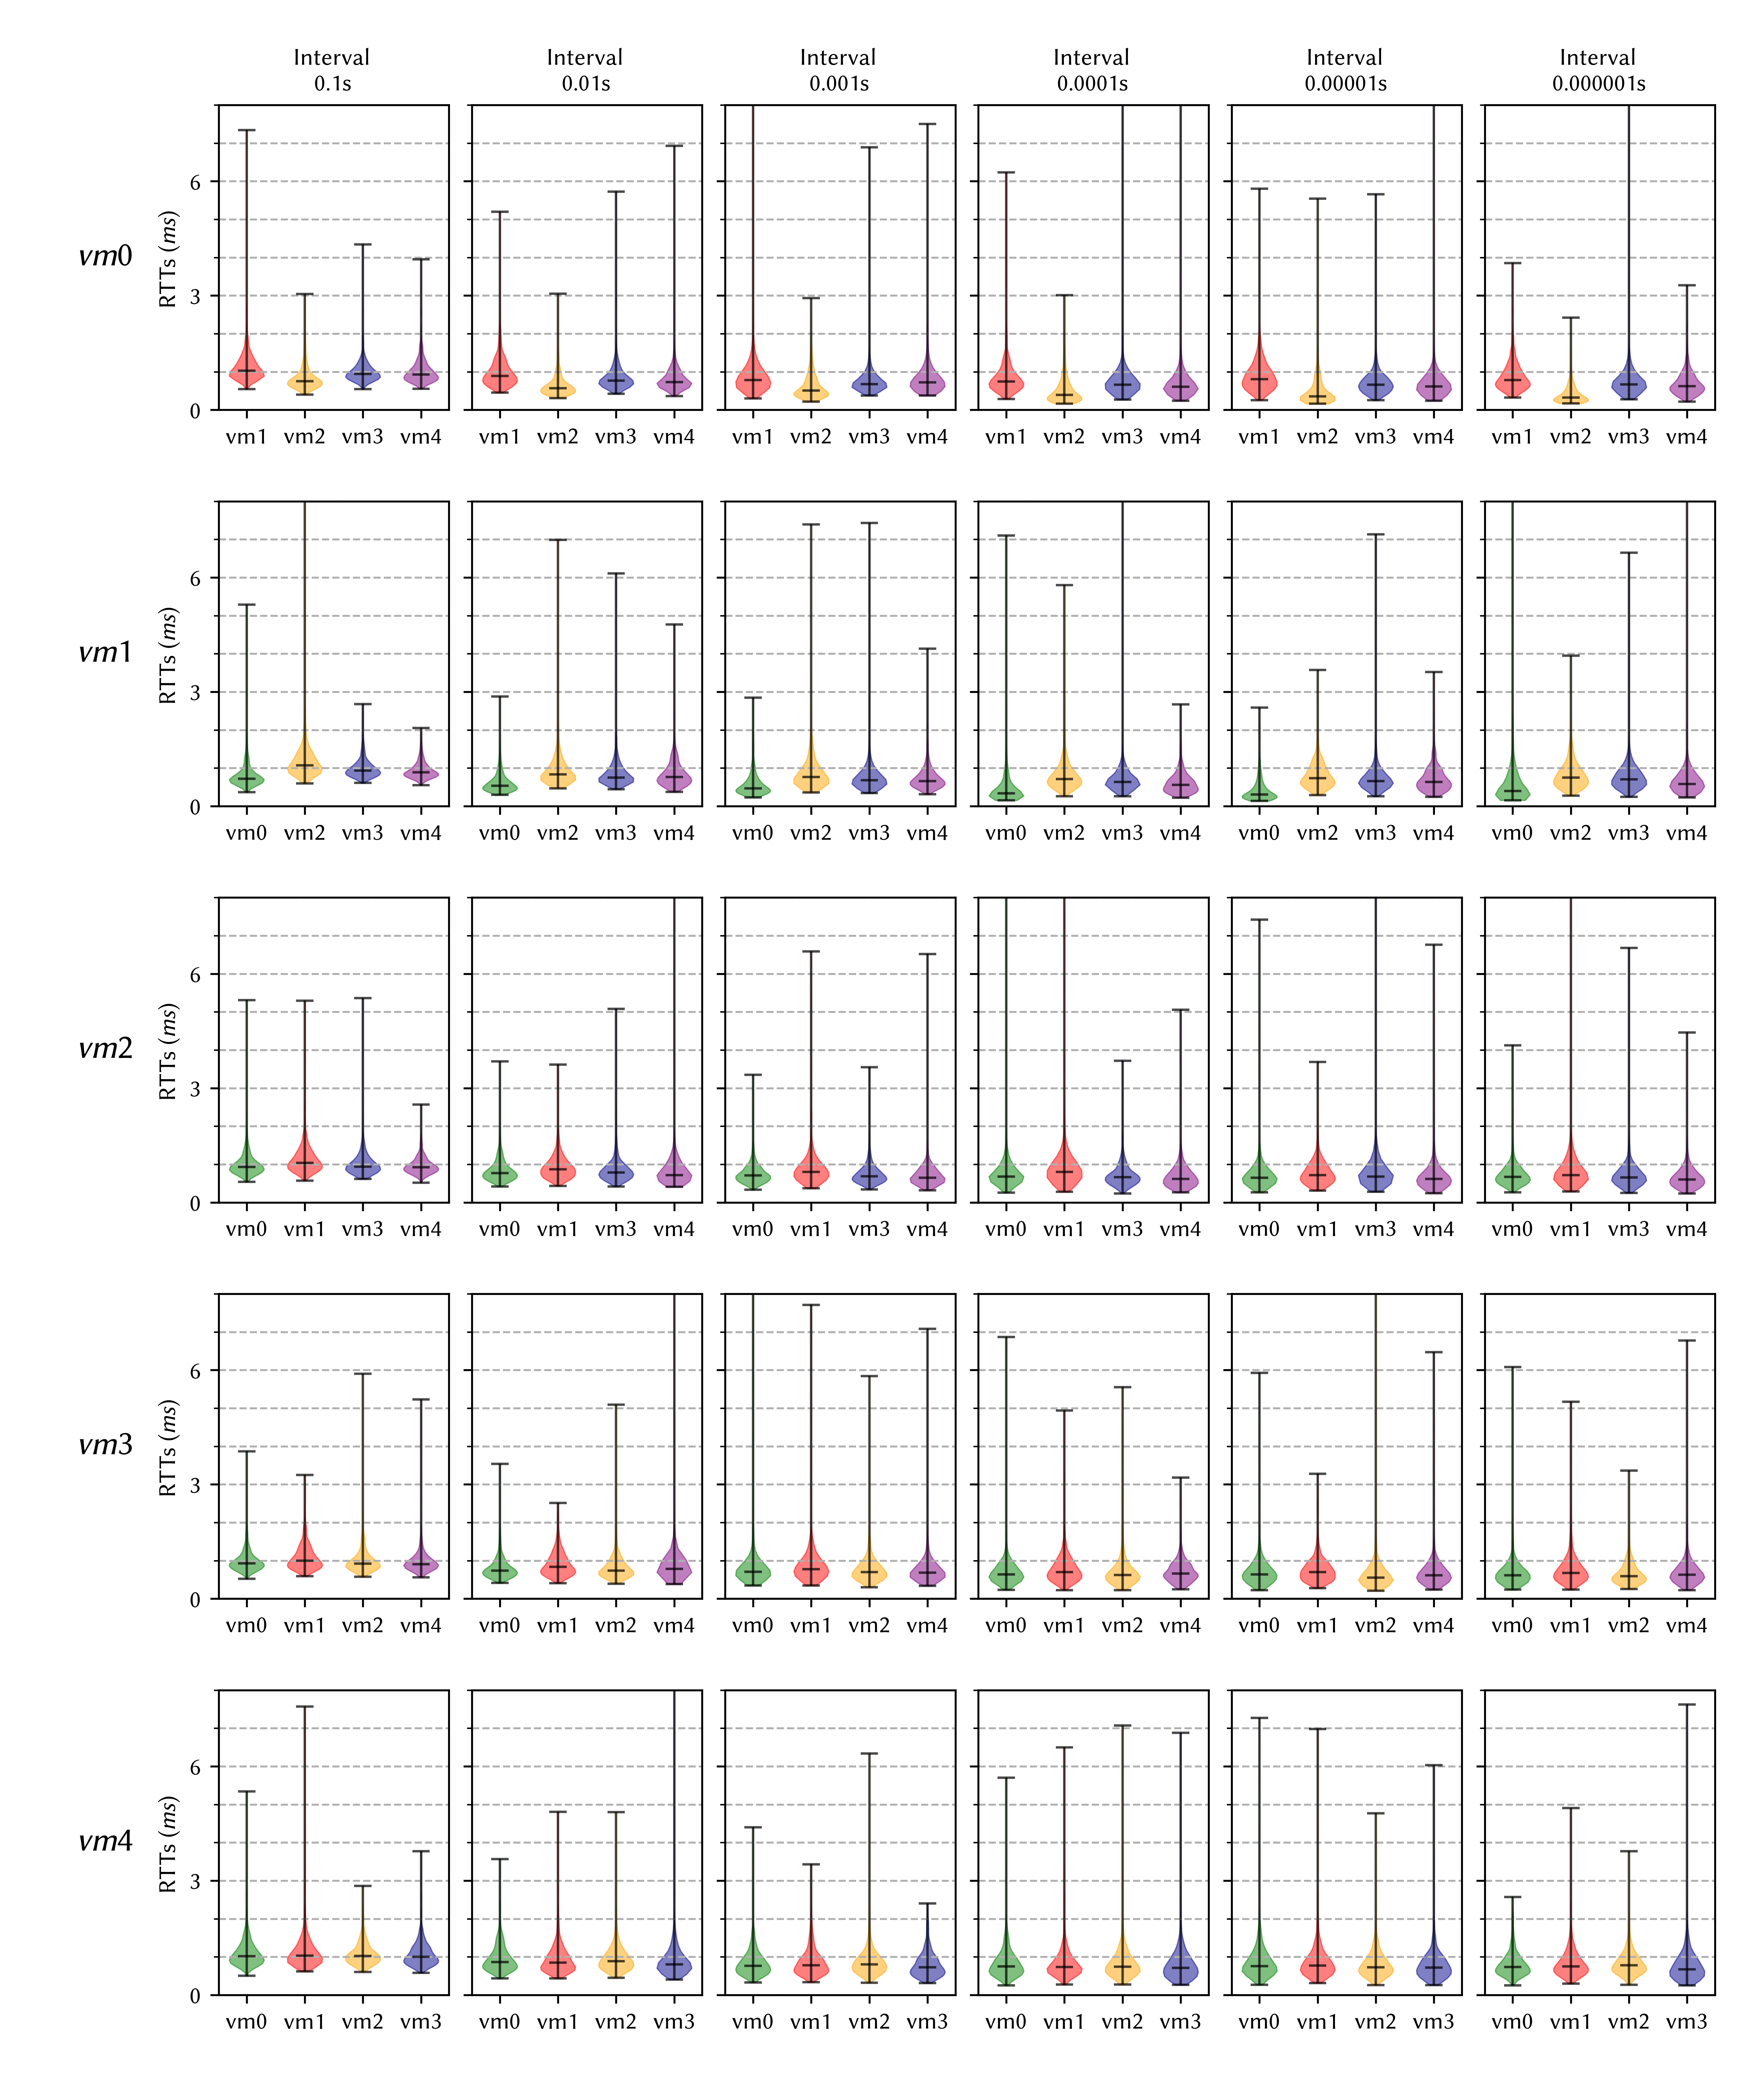
\includegraphics[width=1.15\textwidth]{figs/cluster1/setA/aggr-vis-2-small.png}}%
    \caption{Cluster 1 all-to-all \texttt{ping} performance.}
    \label{fig:ping-c1}
\end{figure}
\begin{figure}
    \centering
    \makebox[\textwidth][c]{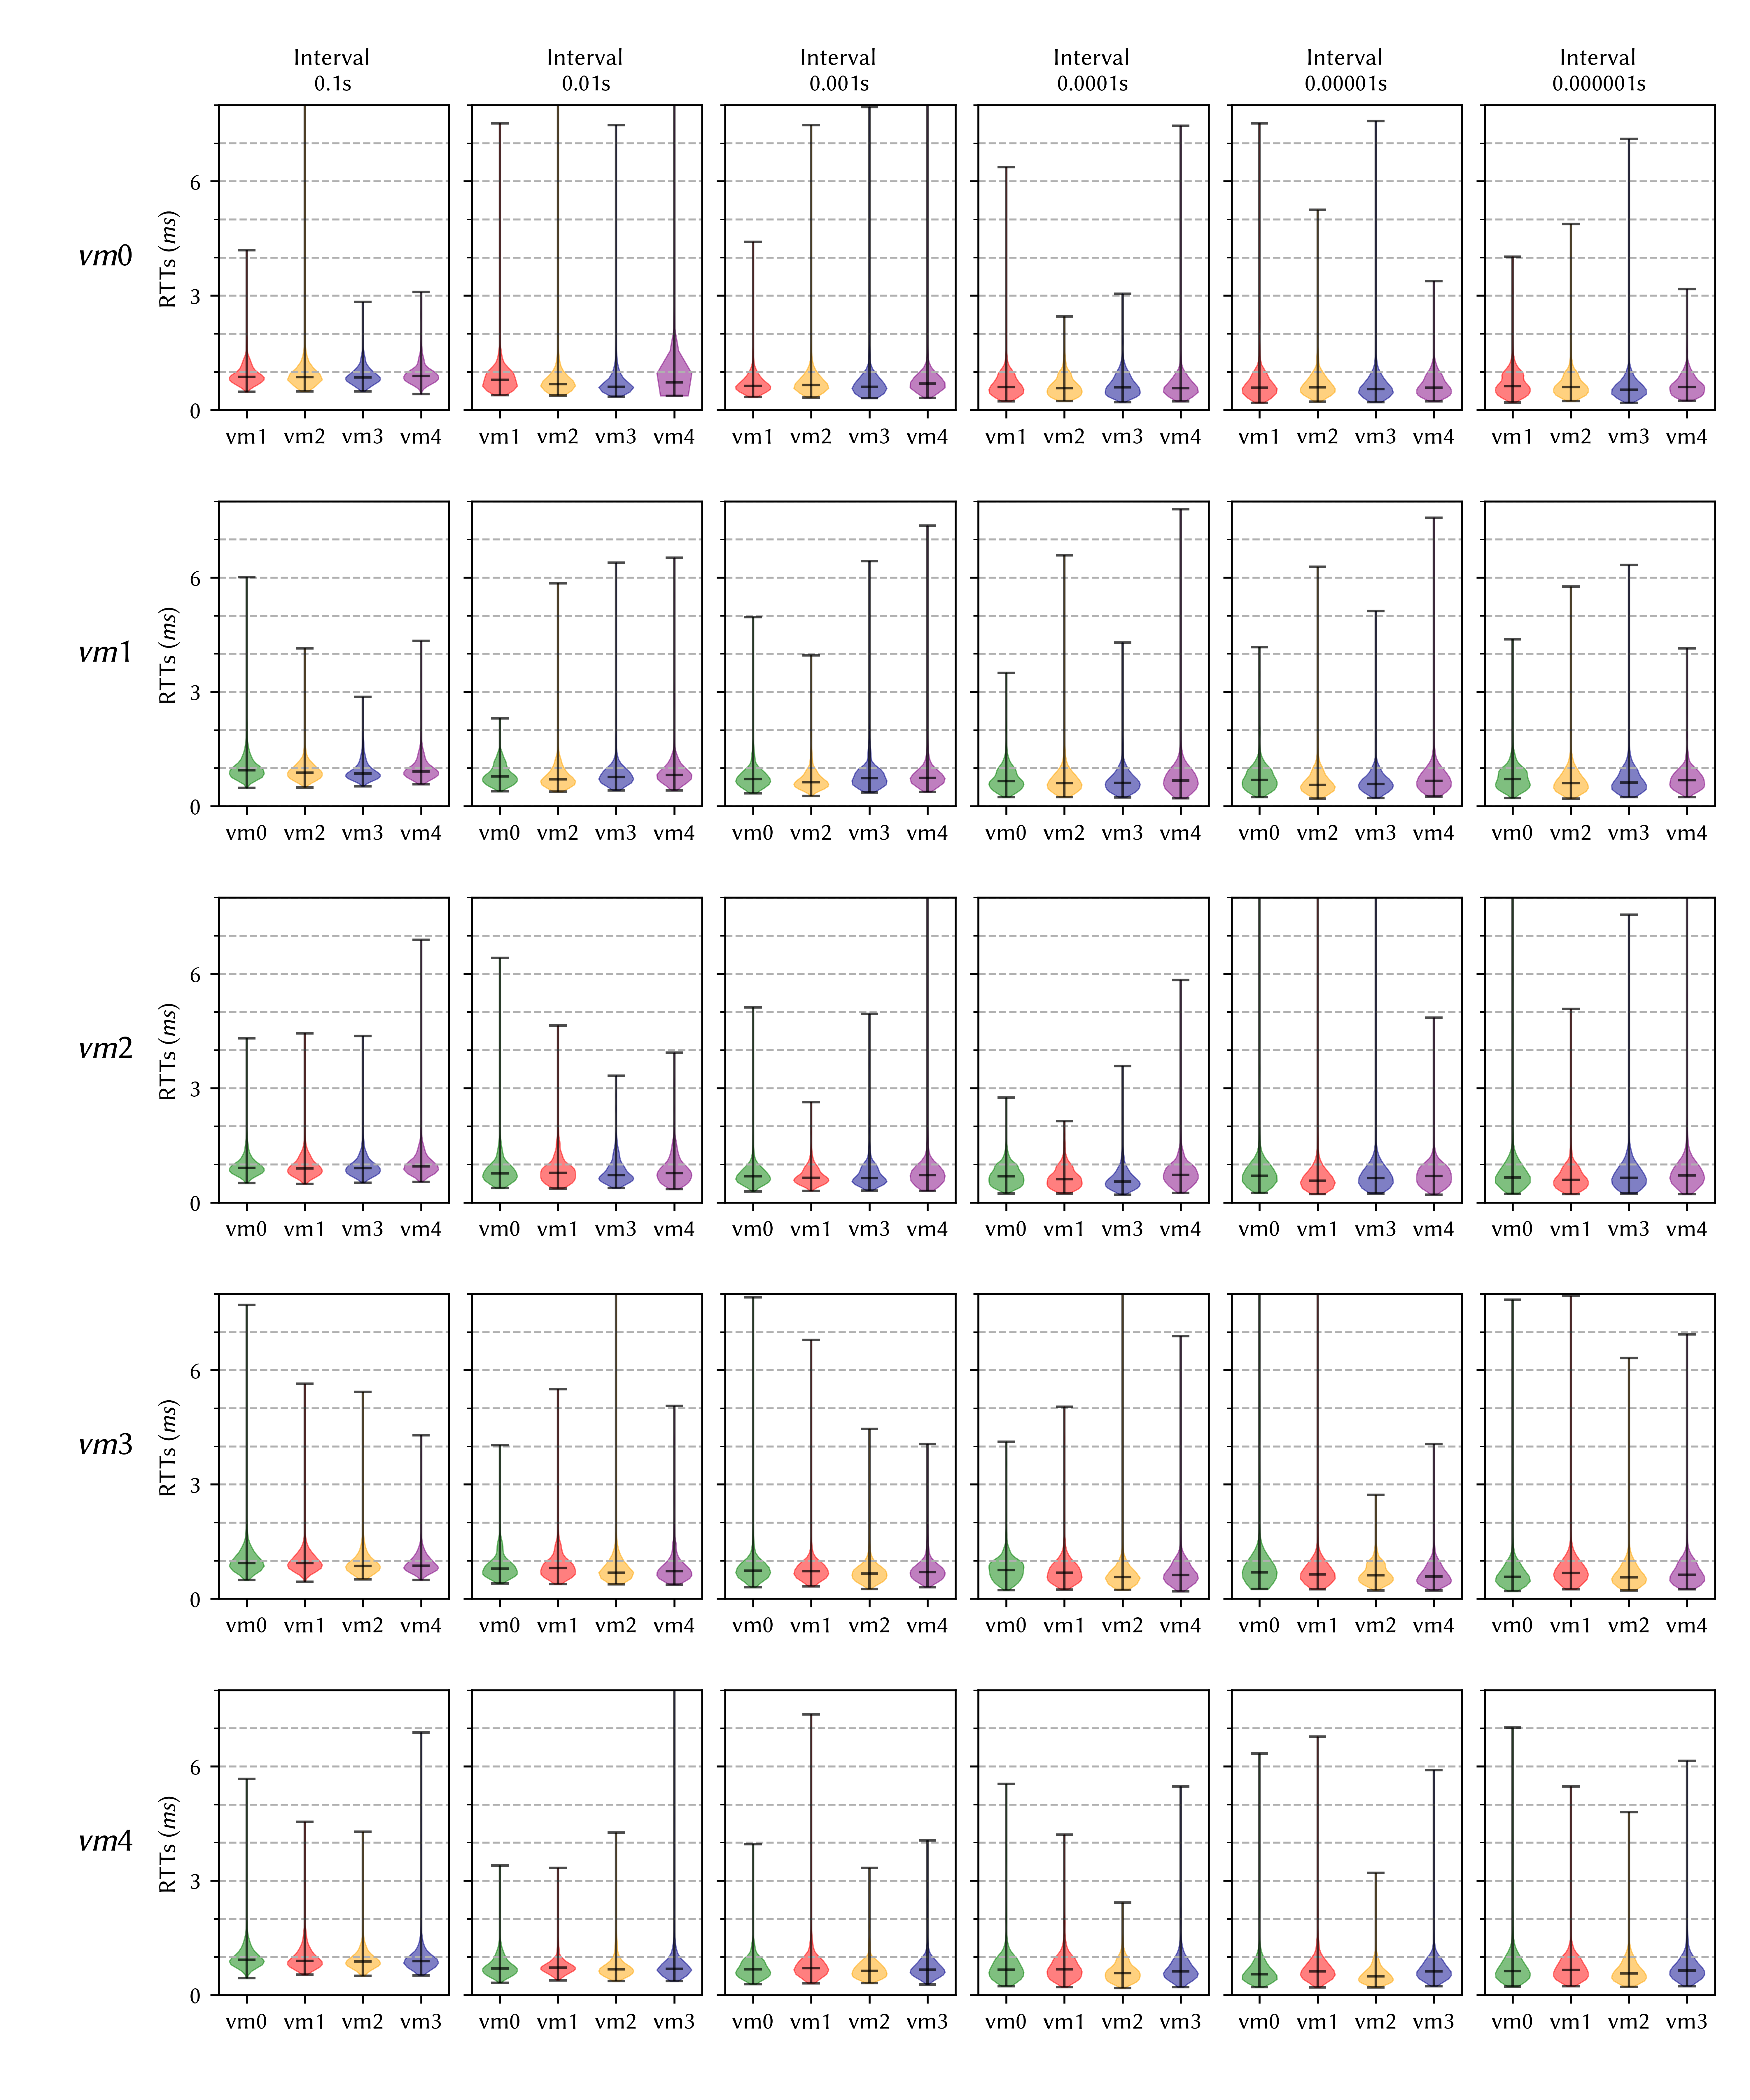
\includegraphics[width=1.15\textwidth]{figs/cluster2/setA/aggr-vis-2-small.png}}%
    \caption{Cluster 2 all-to-all \texttt{ping} performance.}
    \label{fig:ping-c2}
\end{figure}
\clearpage


\newpage
\section{Bandwidth}
\label{sec:bandwidth}

\paragraph{} The framework performs a number of bandwidth exploration experiments; all use \texttt{iperf} or \texttt{iperf3} to drive them. Each attempts to show a different aspect of the VMs' behaviours.
\begin{itemize}
    \item \textbf{Experiment 1} --- simple unidirectional \texttt{iperf} trials between pairs of machines. (TCP/UDP)
    \item \textbf{Experiment 4} --- bidirectional \texttt{iperf} trials between pairs of machines. (TCP/UDP)
    \item \textbf{Experiment 5} --- $n$ to 1 \texttt{iperf3} experiment to ascertain the maximum ingress rate for each machine (sum of all flows). (TCP)
    \item \textbf{Experiment 6} --- 1 to $n$ \texttt{iperf3} experiment to ascertain the maximum egress rate for each machine (sum of all flows, unlike experiment 1 which used only a single flow). (TCP/UDP)
    \item \textbf{Experiment 7} --- identical to experiment 5 but using UDP. This is a separate experiment because of the interesting divergent results it produces.
\end{itemize}

\subsection*{Cluster 1}
\paragraph{Experiment 1} Figure \ref{fig:bw-1} visualises the single-flow maximum egress rate (averaged across all other VMs) for each machine. Figure \ref{fig:bw-1:a} show the results when using TCP: all machines run at 1 Gbps except $vm3$, which runs at 900 Mbps. Similarly, Figure \ref{fig:bw-1:b} shows the results seen when using UDP --- this case is slightly more interesting with the behaviour of $vm0$ and $vm1$. 


\begin{table}[h]
    \centering
    \bgroup
    \def\arraystretch{1.5}%
    \begin{tabularx}{\textwidth}{r|X}
       $vm2$, $vm4$ & These machines are very stable just under 1 Gbps, in line with the results from TCP. \\
       $vm3$ & This appears to settle very quickly and reliably around 850 Mbps, lower than TCP's 900 Mbps. \\
       $vm0$, $vm1$ & From TCP we expect these machines to perform at around 1 Gbps, but instead we see very high-variance readings with an average around 900 Mbps. Both $vm0$ and $vm1$ experienced $26\%-28\%$ packet loss when sending to any of $vm2$, $vm3$, or $vm4$ (at 1 Gbps, so $\sim$730 Mbps received), but $<1\%$ when sending to each other (at $\sim$600 Mbps, 1 Gbps requested). This difference is caused by how the rate limiting manifests itself, and is the reason for the graph being a bit messy.
    \end{tabularx}
    \egroup
\end{table}

\vspace{-3mm}
\paragraph{} This behaviour is consistent across all 8 runs,\footnote{The graphs to verify this are at: \texttt{cluster1/setA/d\{1..8\}/vis/experiment-1/vis-3-\{0..3\}.png}. Two different buffer lengths are tried --- (0, 1) for TCP, (2, 3) for UDP.} suggesting this is not just a noisy reading. This difference in behaviour could suggest that $vm0$ and $vm1$ are logically situated together in a resource pool that applies rate limiting differently on traffic between members and traffic travelling both in and out of it. A low loss rate and low attempted bandwidth ($vm0 \leftrightarrow vm1$) suggest that rate limiting is applied before packets even exit the VM (at the virtual NIC), whereas high loss rates at the requested bandwidth indicates that the rate limiting mechanism proportionally culls packets in-flight when the rate is exceeded.

\begin{figure}
\centering
\begin{subfigure}{.49\textwidth}
  \centering
  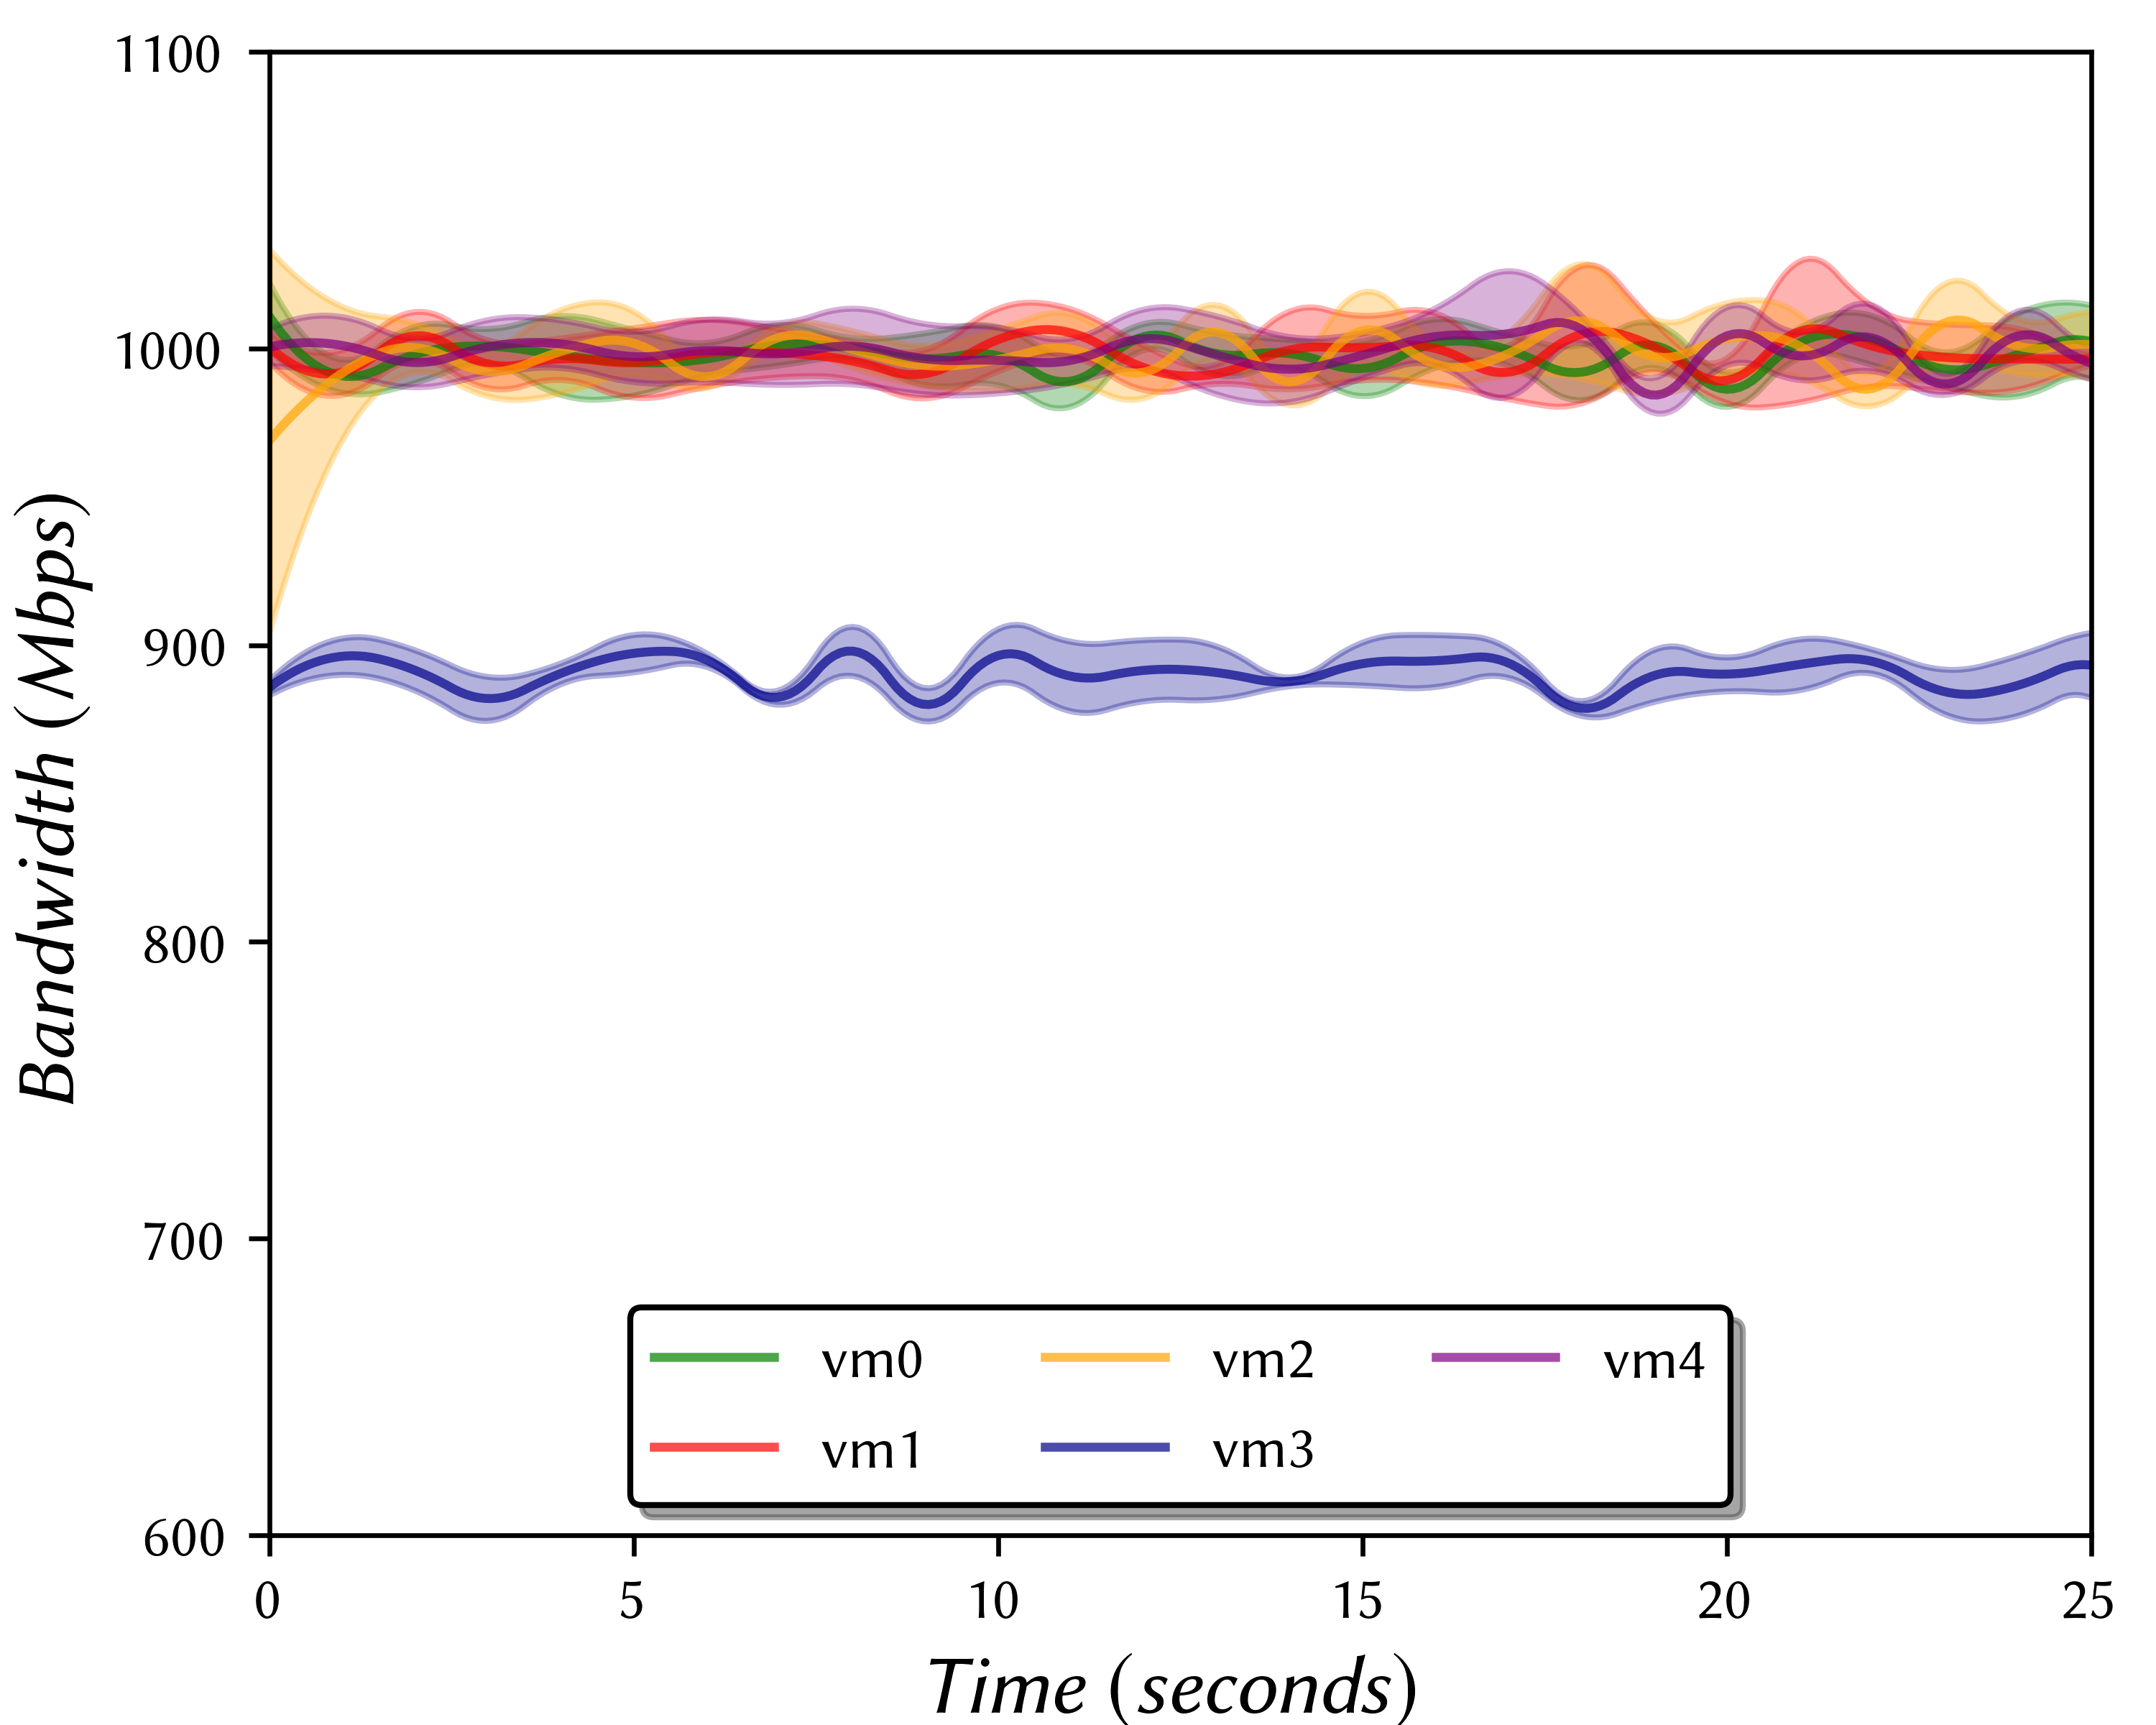
\includegraphics[width=\hsize]{figs/cluster1/setA/vis-3-1.png}
  \caption{TCP bandwidth readings.}
  \label{fig:bw-1:a}
\end{subfigure}%
\hfill%
\begin{subfigure}{.49\textwidth}
  \centering
  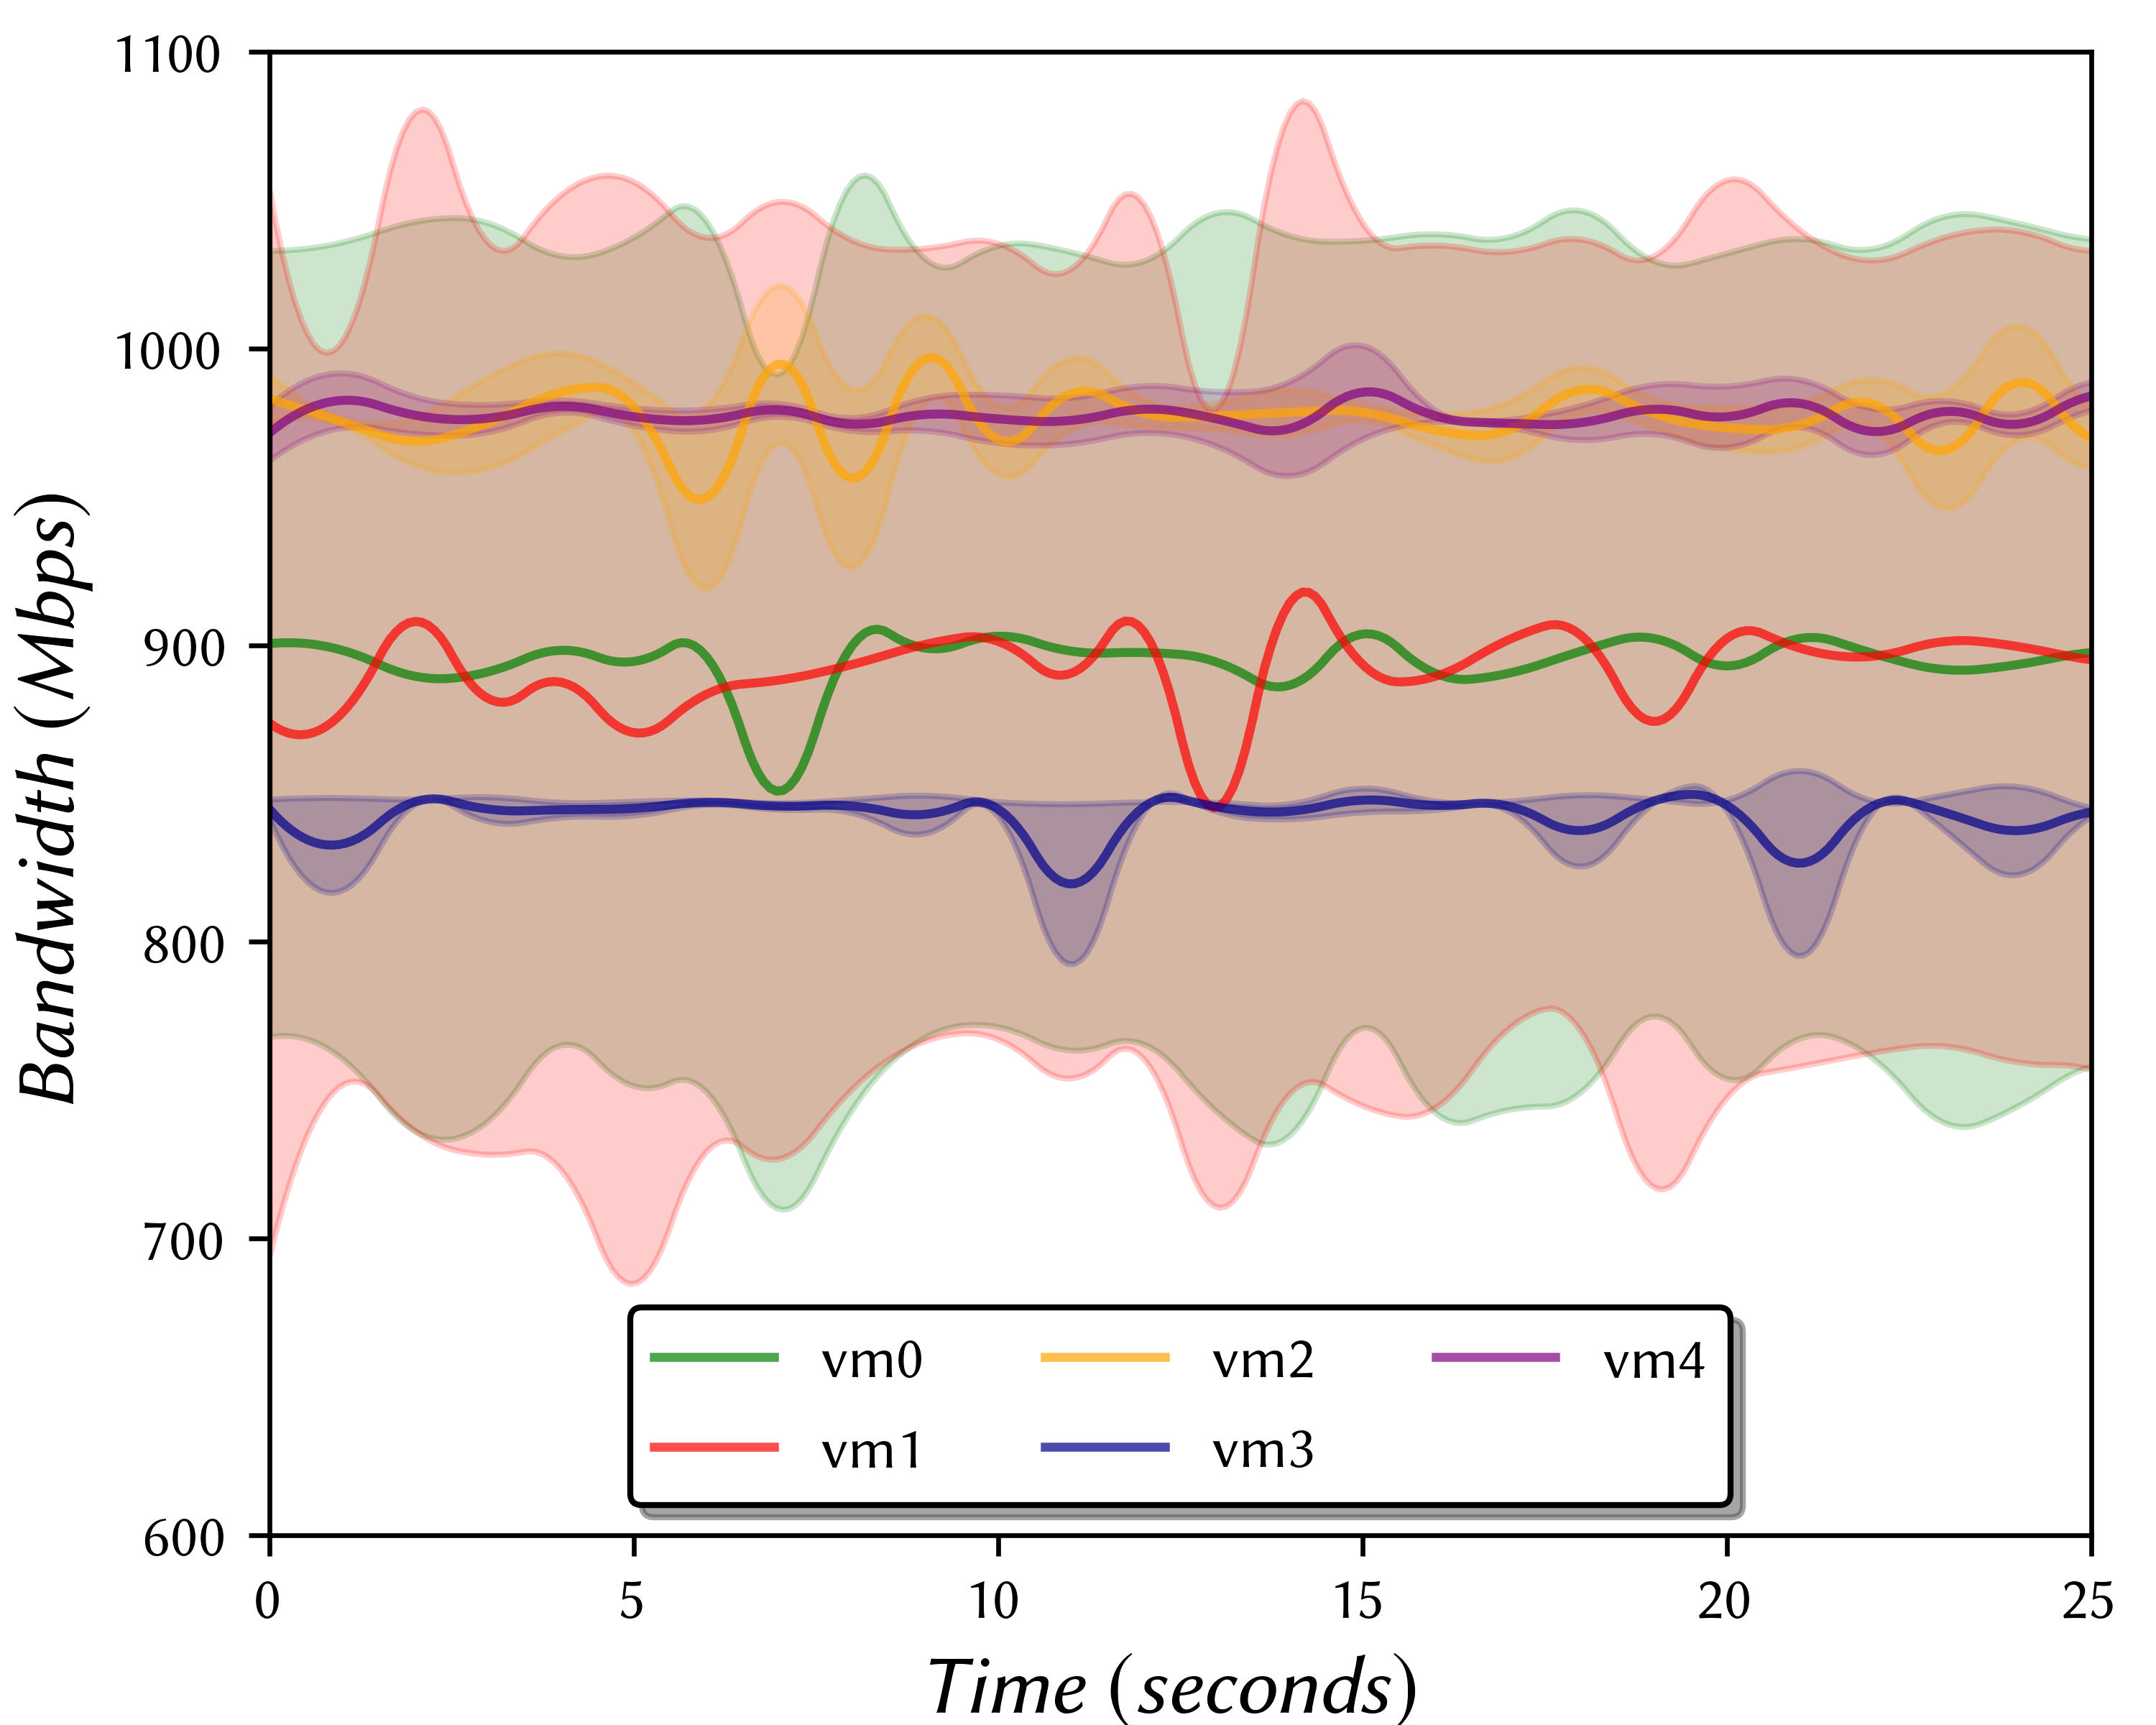
\includegraphics[width=\hsize]{figs/cluster1/setA/vis-3-2.png}
  \caption{UDP bandwidth readings.}
  \label{fig:bw-1:b}
\end{subfigure}%
\caption{\centering{} Cluster 1 VM bandwidths over a 30-second experiment. \\ The first 5 seconds are clipped to allow the network to settle, error bounds are $\pm s$, the sample std. dev. \\ \texttt{cluster1/setA/d8}, Experiment 1 }
\label{fig:bw-1}
\end{figure}

\paragraph{Experiment 4} Figure \ref{fig:bw-bidir-1} (at the end of the section) describes the average observed performances seen for bidirectional \texttt{iperf} trials. The readings for TCP ingress/egress are exactly as expected in relation to Figure \ref{fig:bw-1}, though I would question why $vm3$ exhibits such low variance for TCP ingress --- given we can clearly see it is being rate limited differently to the other machines (at 900 Mbps), this is most likely an artefact of this. For UDP, however, there are a couple of interesting behaviours to note as discussed in the following table.

\begin{table}[h]
    \centering
    \bgroup
    \def\arraystretch{1.5}%
    \begin{tabularx}{\textwidth}{r|X}
       $vm0$, $vm1$ & The observed UDP egress exceeds the ingress values, mirrored in comparison to the other VMs. Whilst this is not enough evidence to draw any conclusions, it adds to the argument made in Experiment 1 that the resource pool $vm0$ and $vm1$ sit in handles rate limiting in a different way to the others, here biasing against ingress traffic. \\
       $vm2$, $vm3$ & The ingress values sit at $\approx$750 Mbps and egress at $\approx$500 Mbps. \\
       $vm4$ & Unlike $vm2$ and $vm3$, this machine's ingress and egress both sit at $\approx$625 Mbps
    \end{tabularx}
    \egroup
\end{table}

\paragraph{} Again, all behaviours are present in all 8 runs, suggesting that they are not just artefacts caused by noise. Every machine's UDP ingress quite closely mirrors UDP egress, reflected in the the line $y = 625$ Mbps. This suggests that the maximum UDP I/O for these machines is around 1.25 Gbps, compared to $\geq$2 Gbps for TCP.

\paragraph{Experiment 5} This experiment attempts to find the maximum ingress rate for each VM, given we have already seen examples of VMs with ingress rates higher than their maximum egress rates. This is achieved by running four experiments per host, in which $n \in \{1,2,3,4\}$ hosts stream data to a single target, reaching up to a theoretical maximum of 4 Gbps ingress. A shown in Figure \ref{fig:bw-n-1-1}, increasing the number of hosts streaming simultaneously to a single machine increases the overall TCP ingress from 1 Gbps to 3-4 Gbps. $vm0$ and $vm2$ are able to receive up to 3.8-3.9 Gbps on average (though this might be increased with more hosts streaming to it, being very close to the 4 Gbps theoretical maximum). $vm1$, $vm3$, and $vm4$ all appear to be limited to $\approx$2.7 Gbps on average. 

\paragraph{} The Azure documentation states that there is no explicit limit on VM ingress bandwidth,\footnote{\url{https://docs.microsoft.com/en-us/azure/virtual-network/virtual-machine-network-throughput}} which raises the question of whether the bottleneck being hit is (a) being quietly imposed by Microsoft, (b) a physical limitation of the machine the VMs are sitting on, or (c) the VM's CPU being unable to handle the traffic rate. (c) is seemingly unlikely, as the B1s VM class is designed to be CPU-burstable up to 3.6 GHz when required; this is fast enough to process up-to and beyond 4 Gbps, as some of the other VMs are already doing. (b) is again unlikely, but when combined with (a) it is feasible that Microsoft implements a fair-use policy, where the NIC's capacity is evenly shared amongst all resident VMs. Speculating along this line of thought, 40 Gbps divides into 2.67 Gbps 15 times, 4 Gbps 10 times, 1.25 Gbps 32 times --- it is not too far fetched to state that $vm0$ and $vm2$ have been assigned a tenth of their physical machine's resource, and $vm1$, $vm3$ and $vm4$ a fifteenth of theirs, by the hypervisor.

\paragraph{Experiment 6} In a similar vein to Experiment 5, Experiment 6 asks whether the maximum egress value we've seen is per-flow or per-machine. For this trial, $n \in \{1,2,3,4\}$ \texttt{iperf3} instances run simultaneously on a VM, all streaming to different hosts. Figure \ref{fig:bw-1-n-1} plots the average observed behaviour. The conclusion is simple; the 1 Gbps egress rate limit (900 Mbps for $vm3$) is not per-flow, but for the entire machine. We see the bandwidth achieved by each sending process decrease to $1000 \cdot n^{-1}$ Mbps when $n$ processes are actively sending. The results are near identical for UDP, though the total bandwidth is reliably in the 900-1000 Mbps range for all machines, unlike the volatile single flow figures reported in Figure \ref{fig:bw-1:b}. 

\paragraph{Experiment 7} As already stated, Experiment 7 is identical to Experiment 5 but using UDP. The reason for splitting this out is because it appears that either the VMs or both \texttt{iperf} and \texttt{iperf3} are unable to handle multiple incoming 1 Gbps UDP streams at once. This is rather peculiar, as \texttt{iperf} reports that each of the $n \in \{2,3,4\}$ clients connects successfully, but then reports that all bar a handful of packets are lost (loss rate $\gt 99\%$).\footnote{The \texttt{iperf} outputs for these experiments are saved in \texttt{data/cluster1/setA/d\{1..8\}/..-experiment7/}.} This happens with both \texttt{iperf} and \texttt{iperf3}, both when run manually or automatically, suggesting this is an issue with/configuration choice to disallow this traffic pattern of the VMs themselves.

\subsection*{Cluster 2}
\paragraph{} Many of the experiment specifics for Cluster 2 are identical to those already discussed for Cluster 1. This section very briefly discusses the differences seen from Cluster 2 --- no interesting anomalies were observed.

\paragraph{Experiment 1} Figure \ref{fig:bw-2} shows how all machines in Cluster 2 exhibit 1 Gbps maximum TCP egress, and, although more variable, 1 Gbps for UDP egress. No VMs show any anomalous behaviour.


\begin{figure}
\centering
\begin{subfigure}{.49\textwidth}
  \centering
  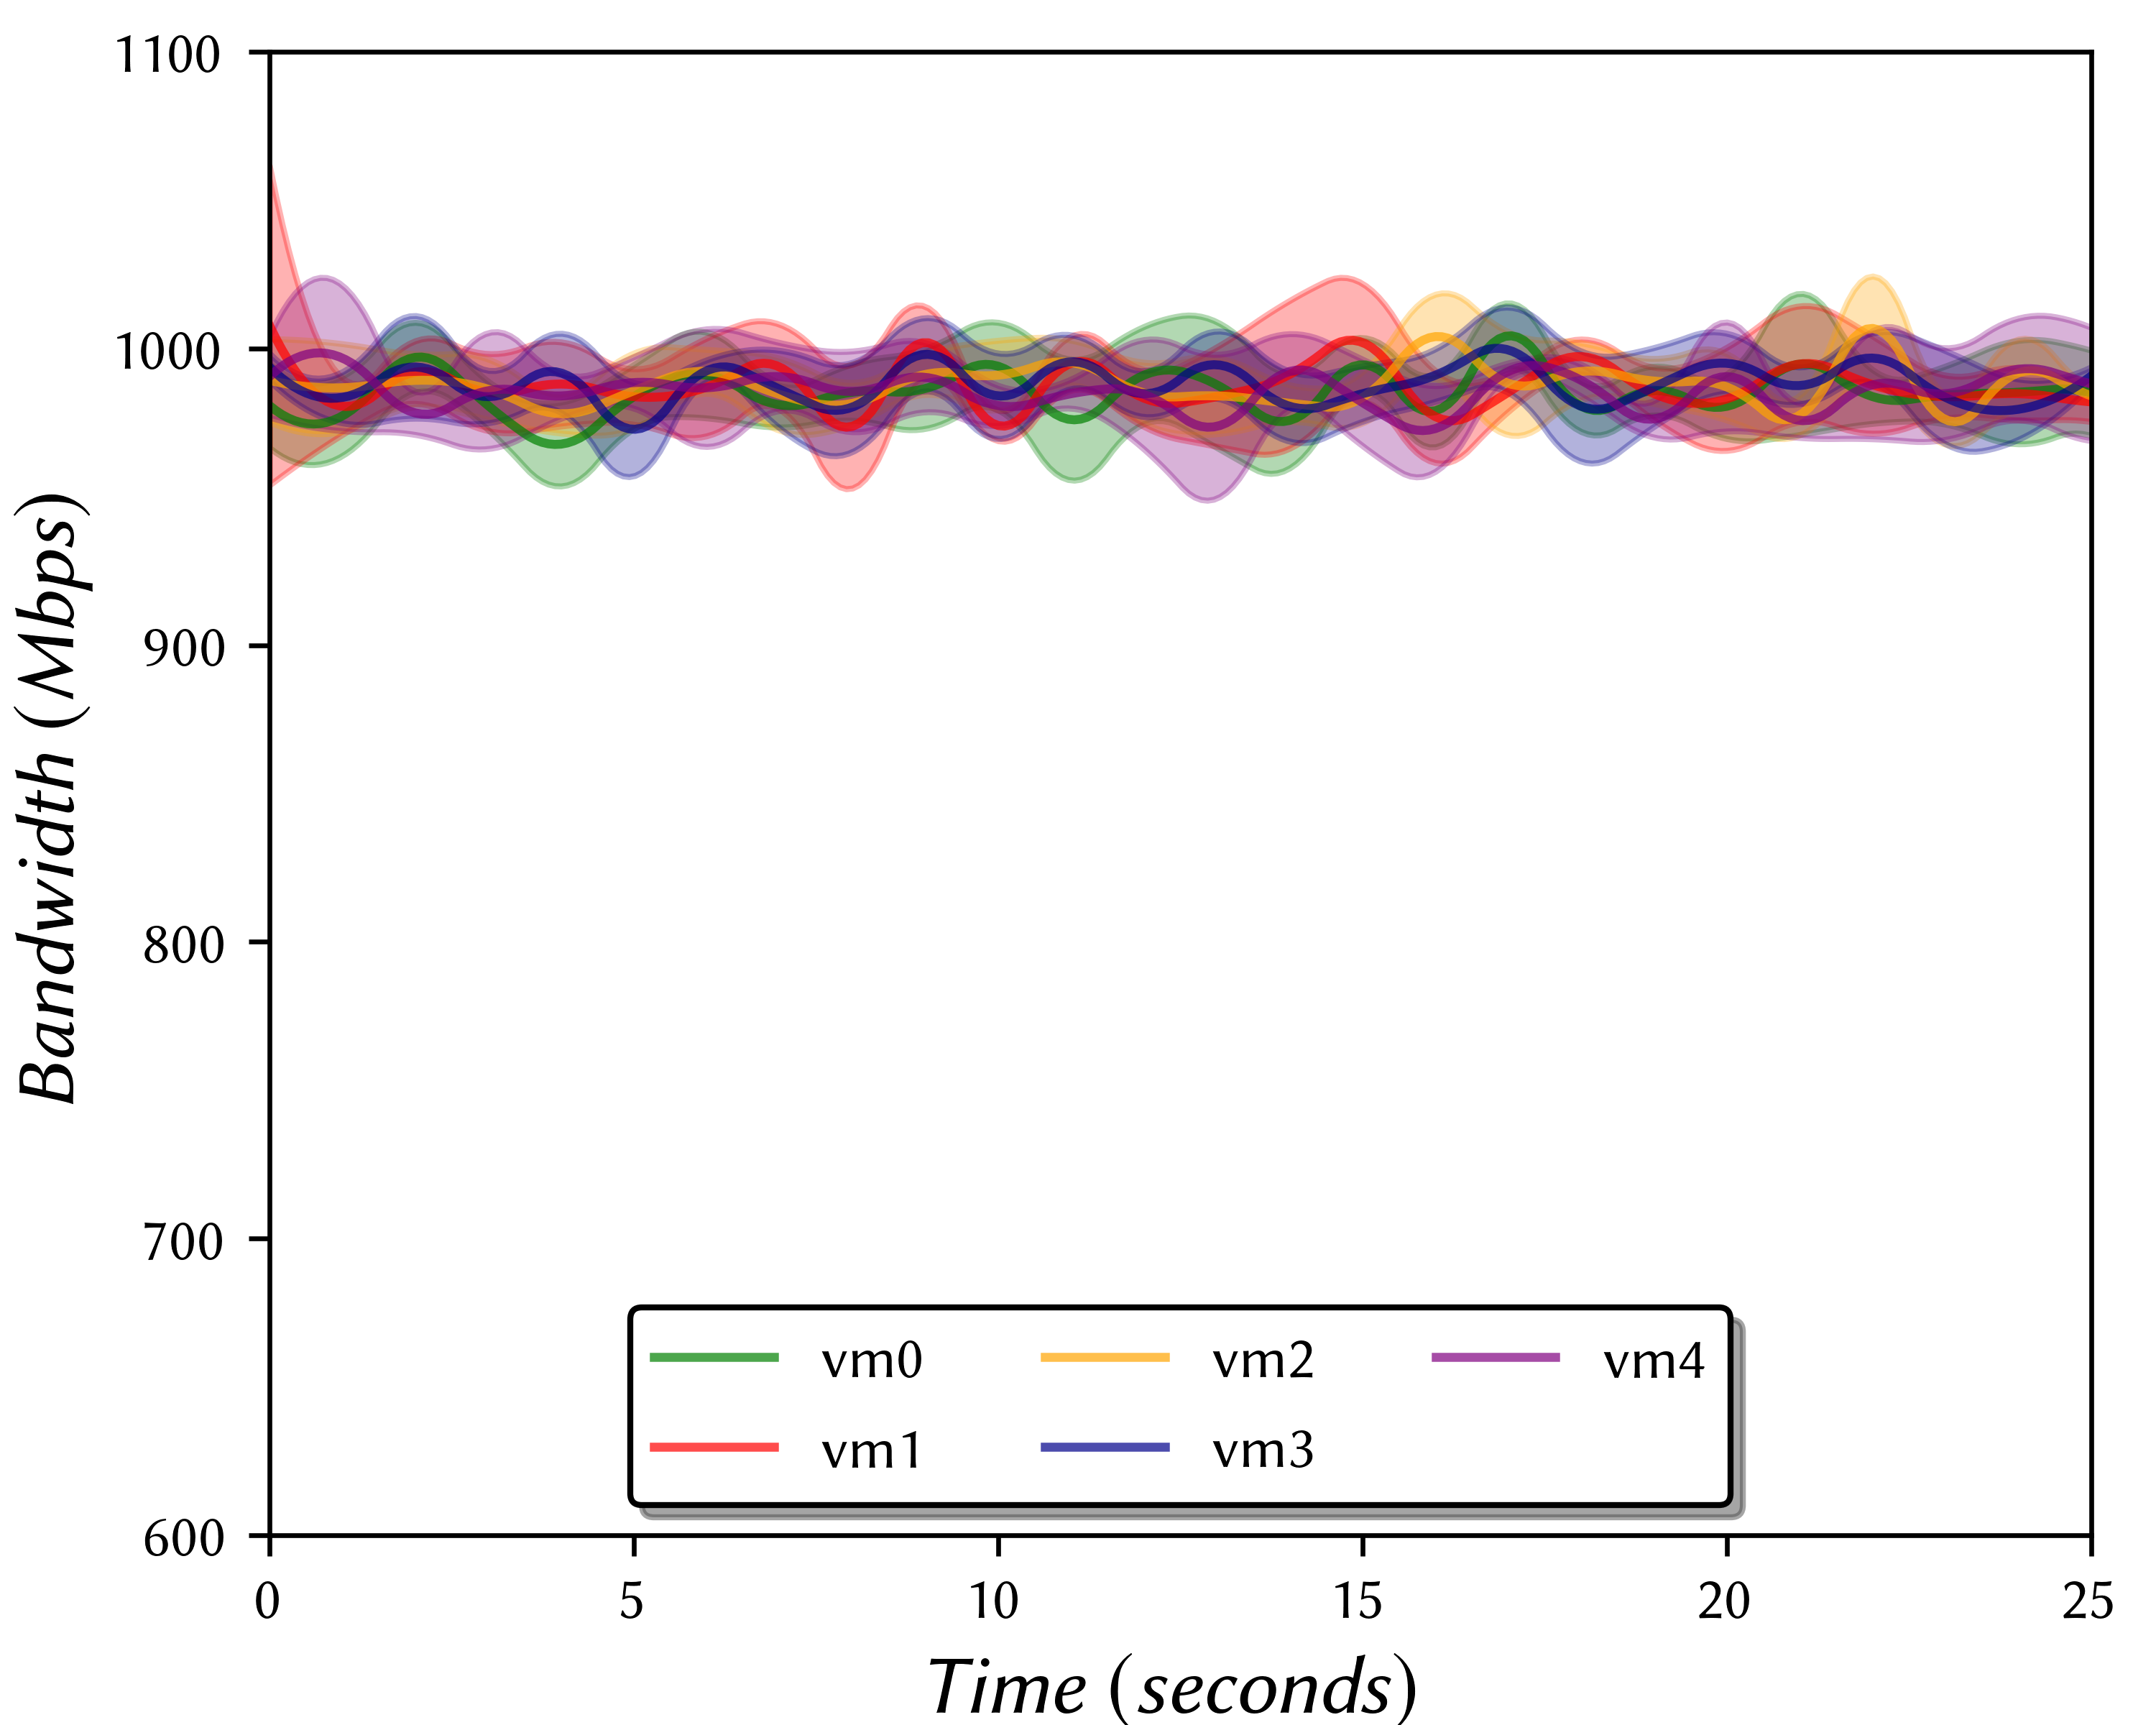
\includegraphics[width=\hsize]{figs/cluster2/setA/vis-3-1.png}
  \caption{TCP bandwidth readings.}
  \label{fig:bw-2:a}
\end{subfigure}%
\hfill%
\begin{subfigure}{.49\textwidth}
  \centering
  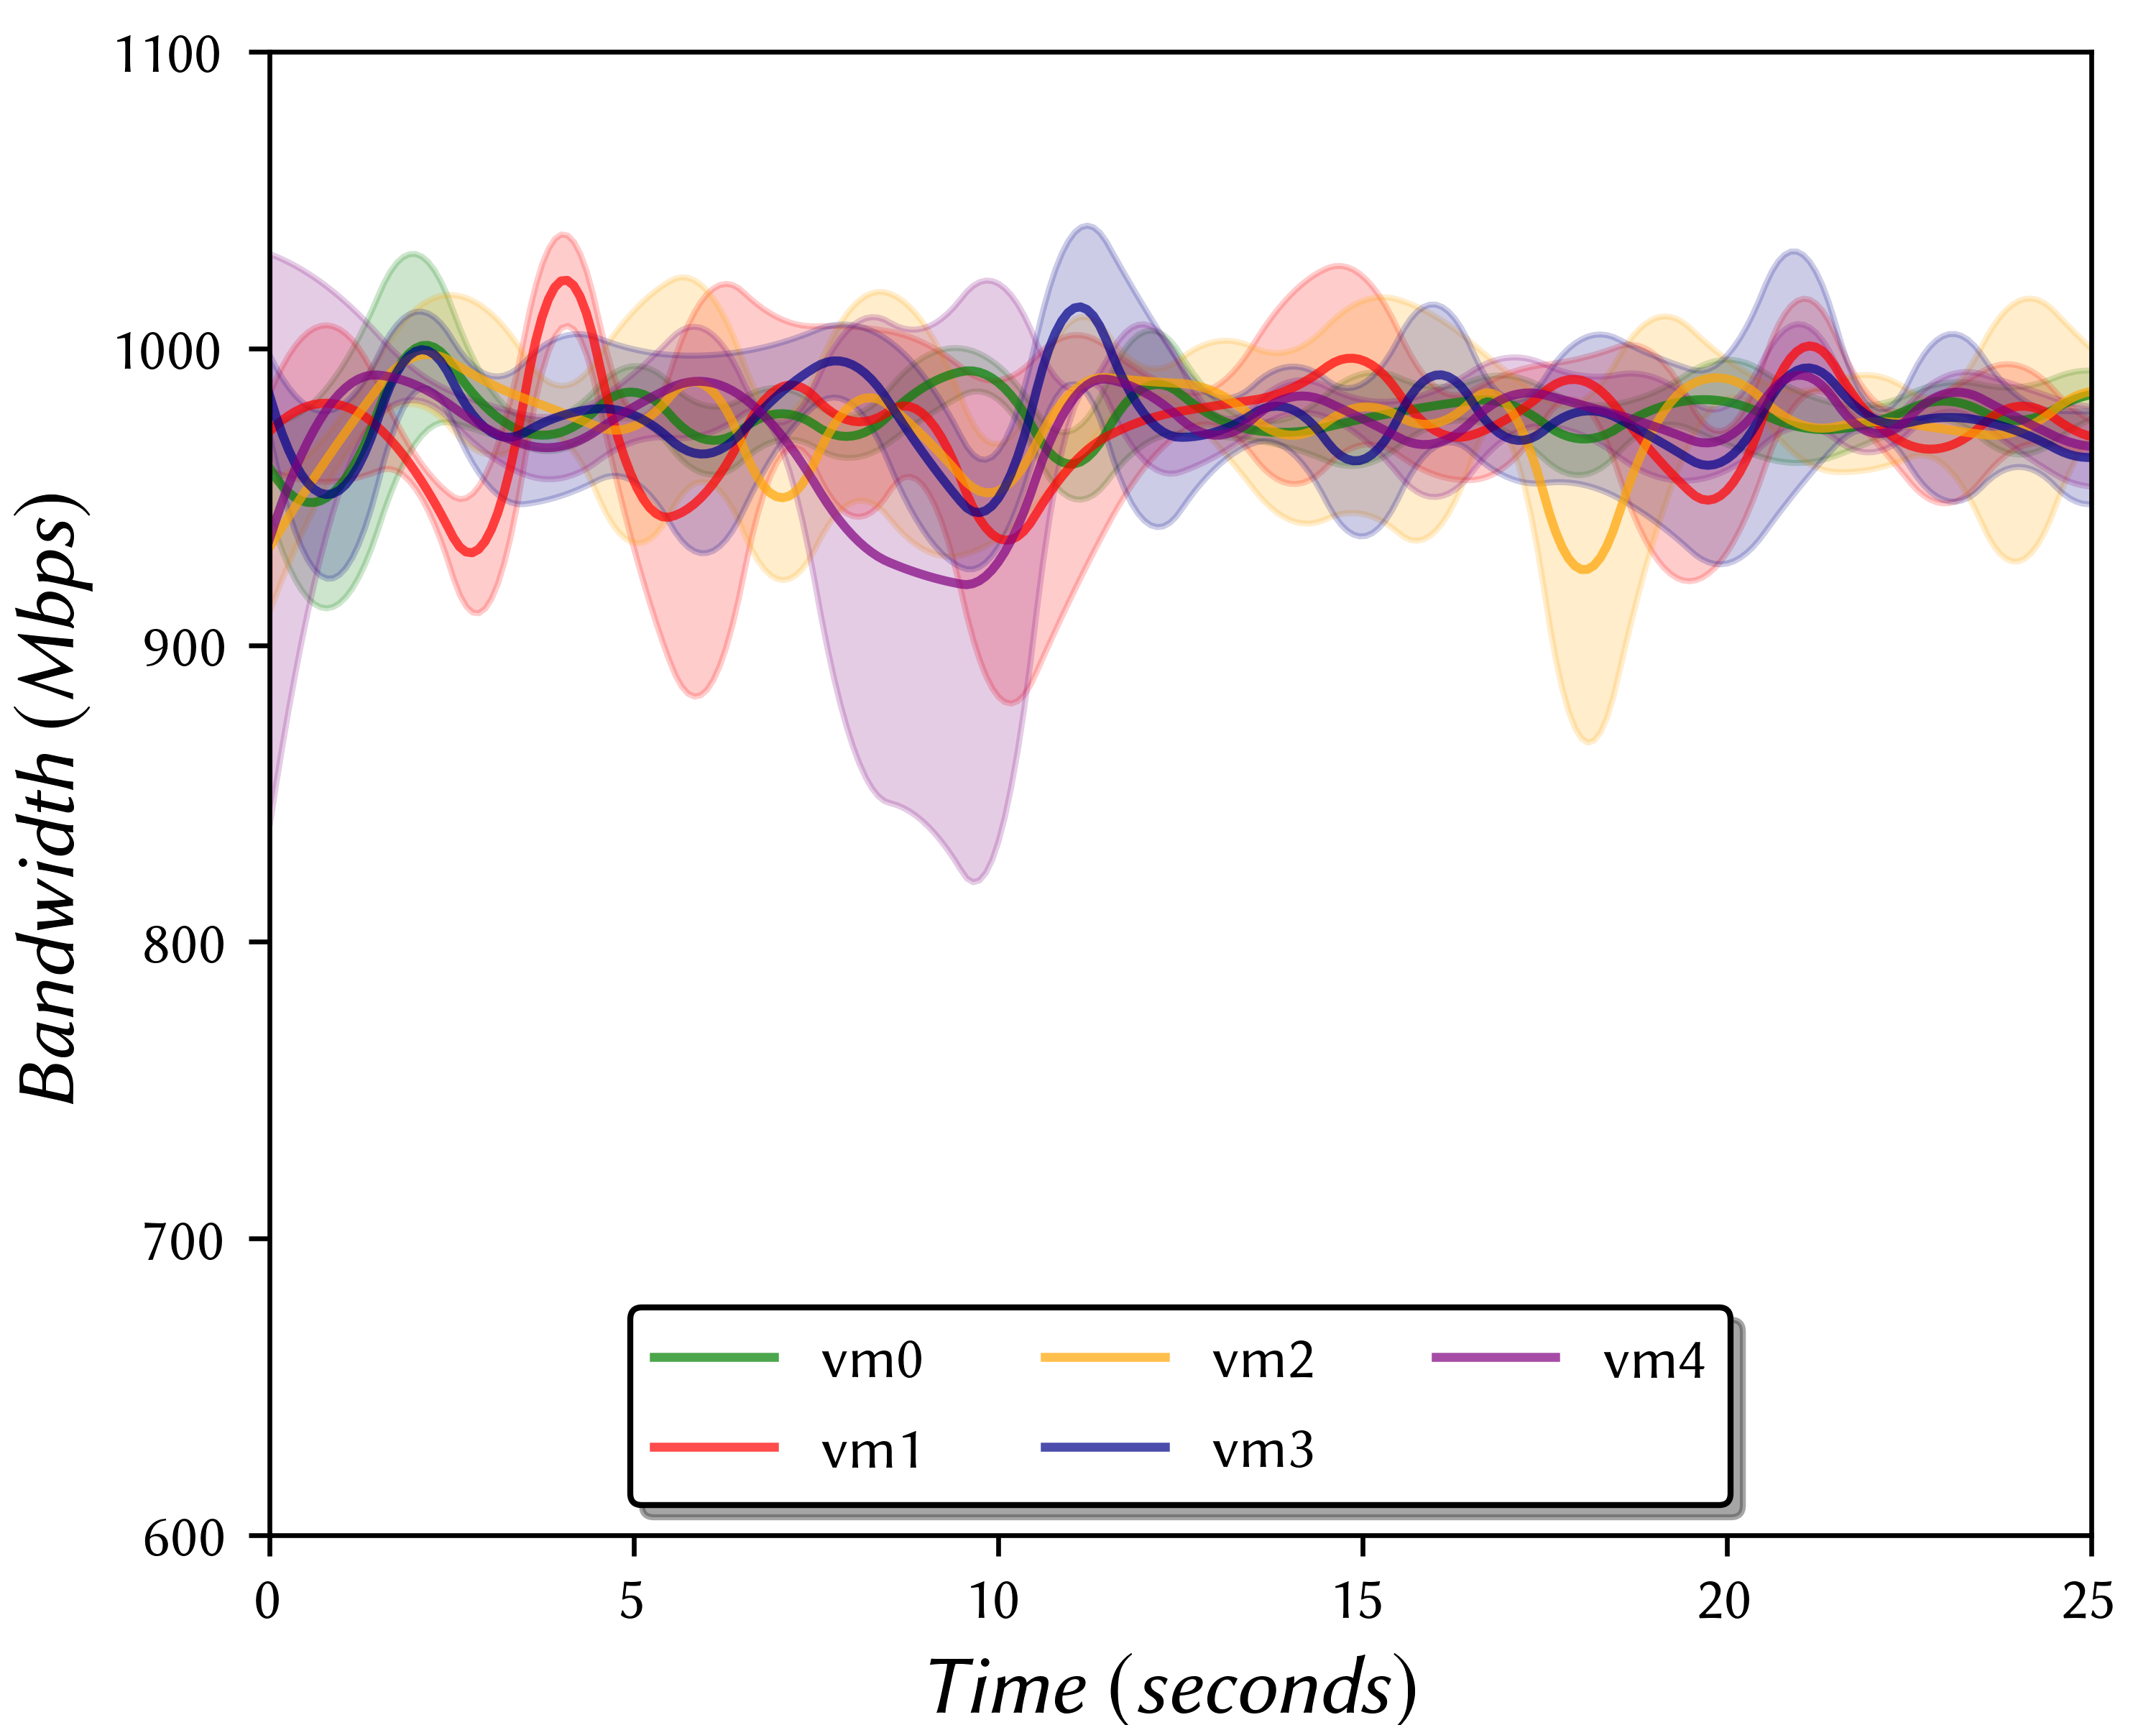
\includegraphics[width=\hsize]{figs/cluster2/setA/vis-3-2.png}
  \caption{UDP bandwidth readings.}
  \label{fig:bw-2:b}
\end{subfigure}%
\caption{\centering{} Cluster 2 VM bandwidths over a 30-second experiment. \\ The first 5 seconds are clipped to allow the network to settle, error bounds are $\pm s$, the sample std. dev. \\ \texttt{cluster2/setA/d8}, Experiment 1 }
\label{fig:bw-2}
\end{figure}


\paragraph{Experiment 4} Exactly as seen with Cluster 1, Figure \ref{fig:bw-bidir-2} shows TCP ingress/egress reliably fixed at 1 Gbps. Further, the average sum of UDP ingress and egress streams is $\approx$1250 Mbps, as before. $vm0$ and $vm4$ are the only two VMs with UDP egress greater than its ingress: we saw this phenomenon in Cluster 1 as well, where we tentatively ascribed it to the two VMs residing in the same resource cluster with different rate limiting techniques being used. The case for this is not as strong this time, as, with reference to Figure \ref{fig:ping-dist-2}, these two machines do not appear to have a particularly strong locality correlation --- no concrete conclusion can be drawn, but it is clear that the traffic for these two node is being manipulated in a different way to the others.

\paragraph{Experiment 5} Figure \ref{fig:bw-n-1-2} demonstrates that every VM in Cluster 2 has an upper TCP ingress ceiling of between 2.7-2.9 Gbps on average, a fifteenth of their physical NIC's capacity.

\paragraph{Experiments 6 and 7} Figure \ref{fig:bw-1-n-2} is, again, nearly identical to the results seen for Cluster 1; the 1 Gbps egress rate limit apply across all flows, not just per-flow. Cluster 2 exhibits the same behaviour as Cluster 1 for multiple UDP ingress streams; it culls all of them, resulting in $\gt 99\%$ packet loss.


\clearpage


\begin{figure}
\centering
\begin{subfigure}{.33\textwidth}
  \centering
  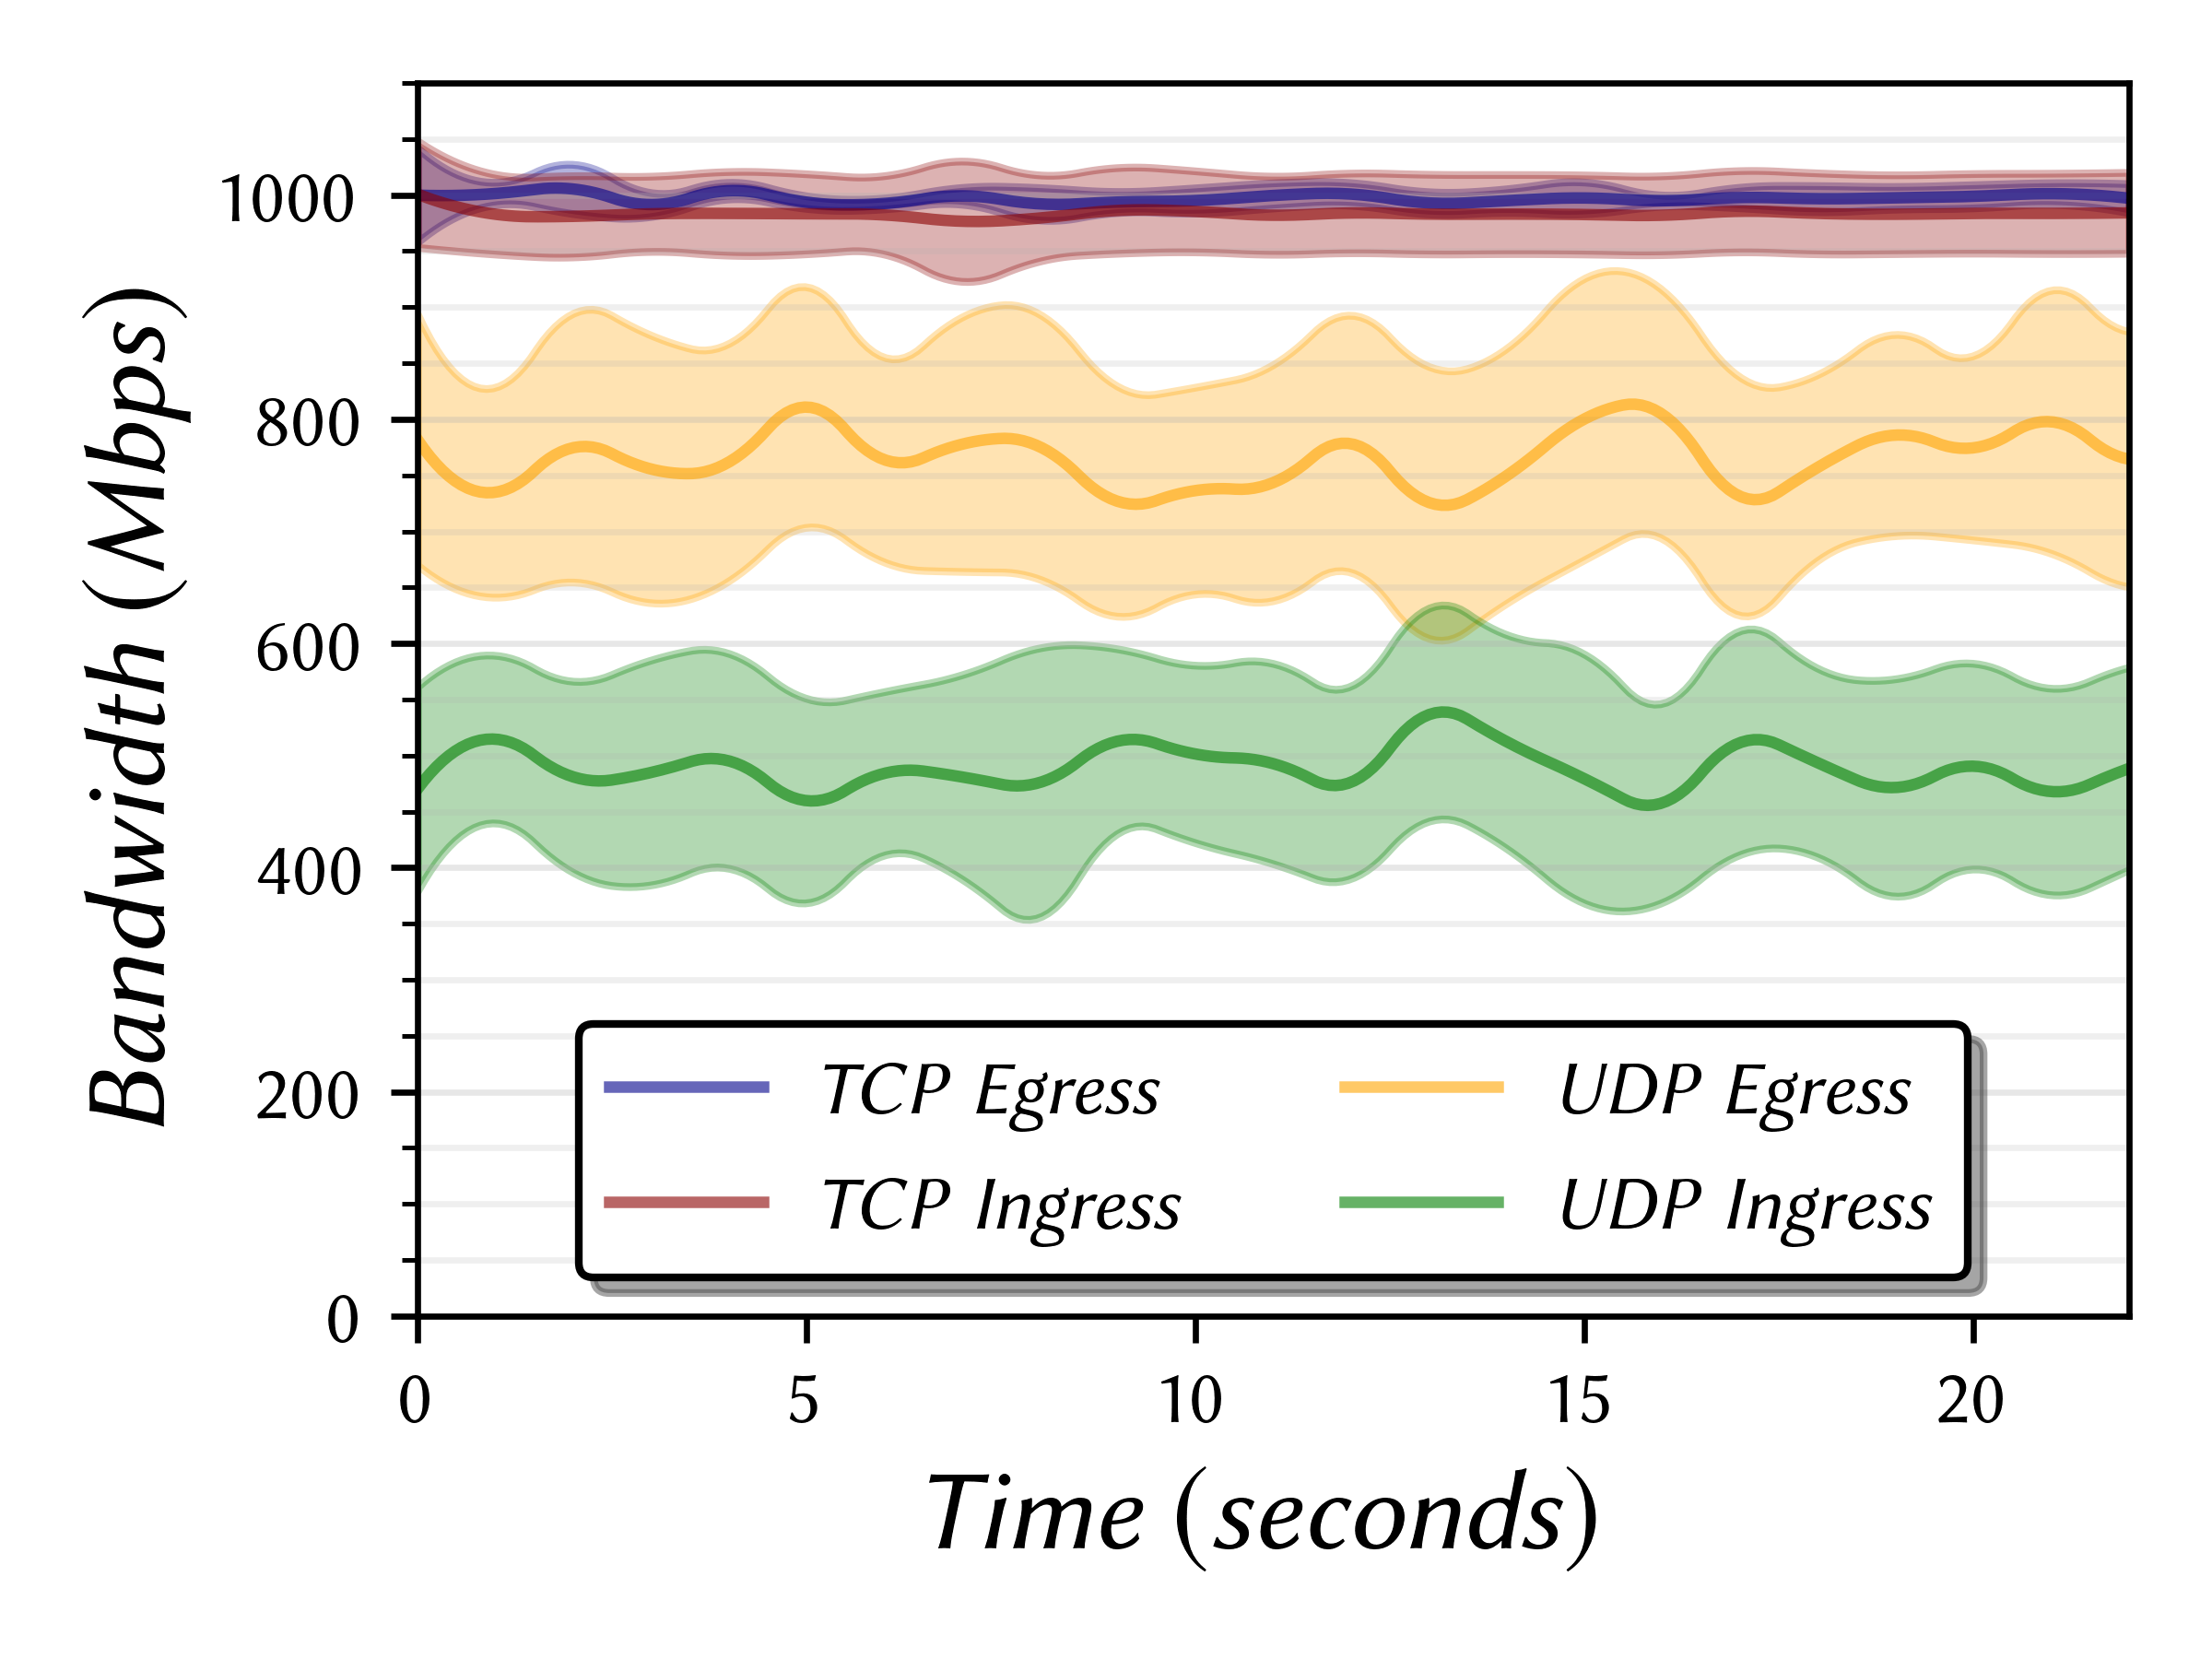
\includegraphics[width=\hsize]{figs/cluster1/setA/vis-5-vm0-combined.png}
  \caption{$vm0$}
  \label{fig:bw-bidir-1:a}
\end{subfigure}%
\hfill%
\begin{subfigure}{.33\textwidth}
  \centering
  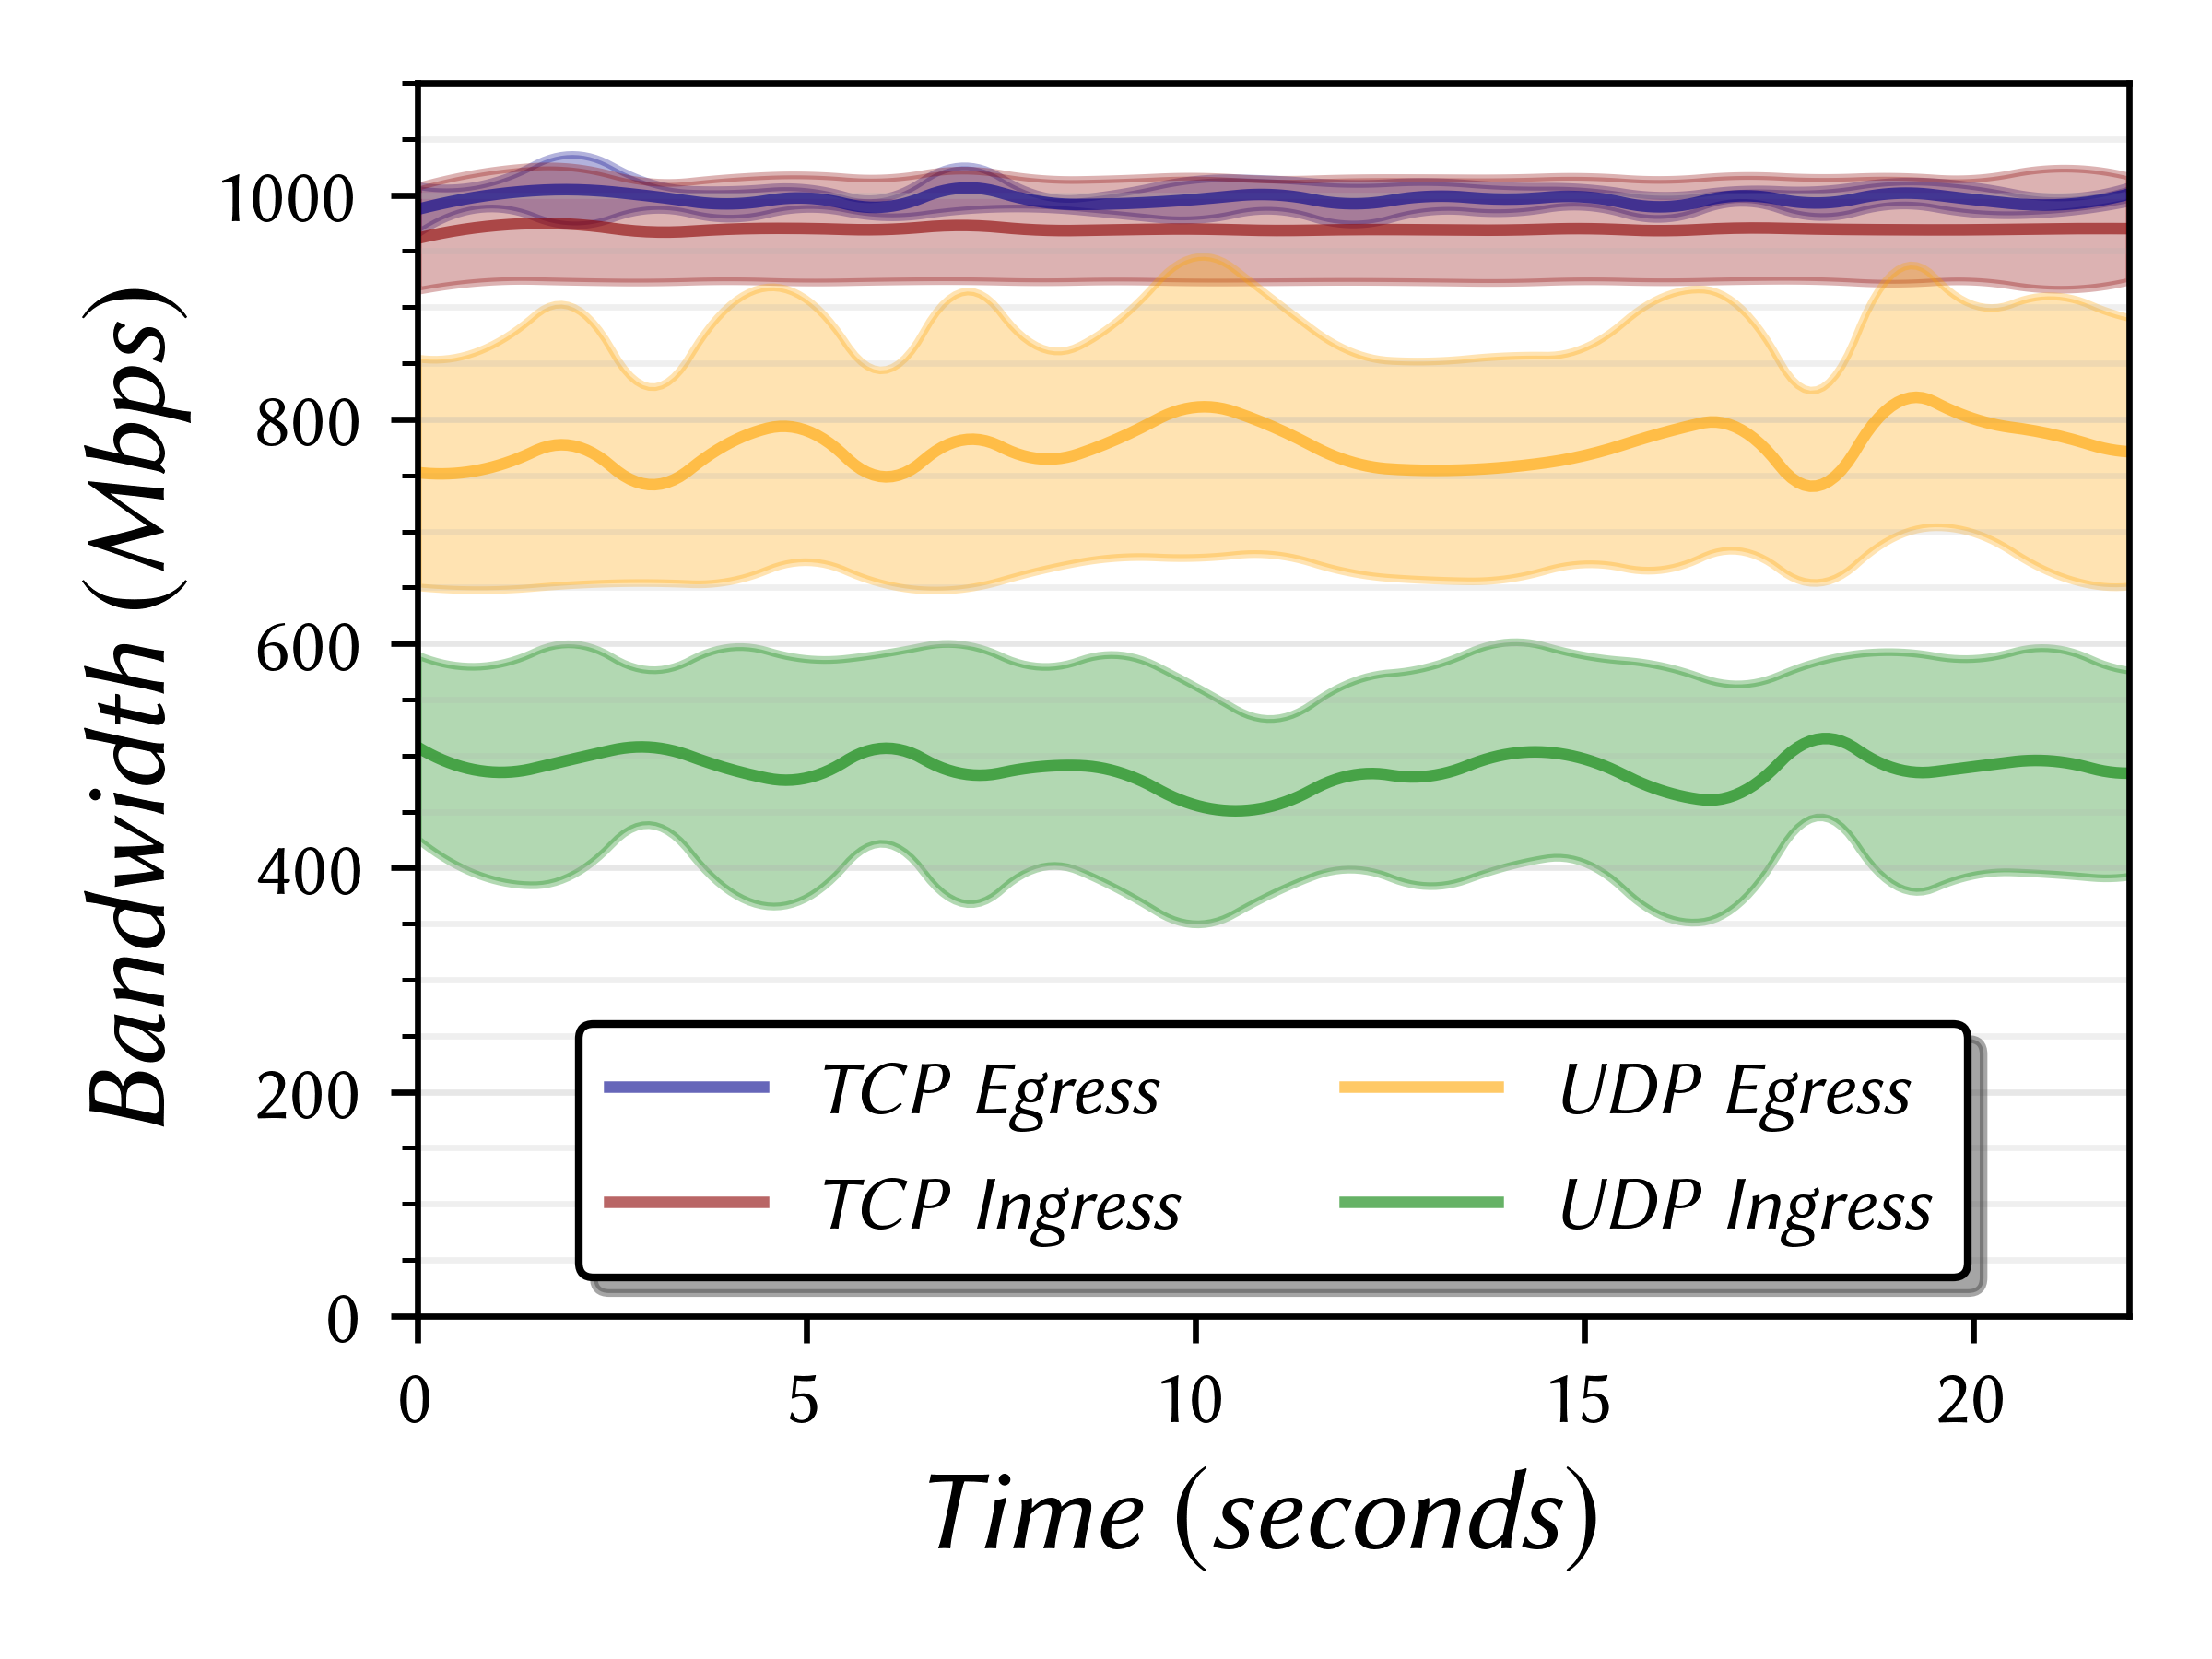
\includegraphics[width=\hsize]{figs/cluster1/setA/vis-5-vm1-combined.png}
  \caption{$vm1$}
  \label{fig:bw-bidir-1:b}
\end{subfigure}%
\hfill%
\begin{subfigure}{.33\textwidth}
  \centering
  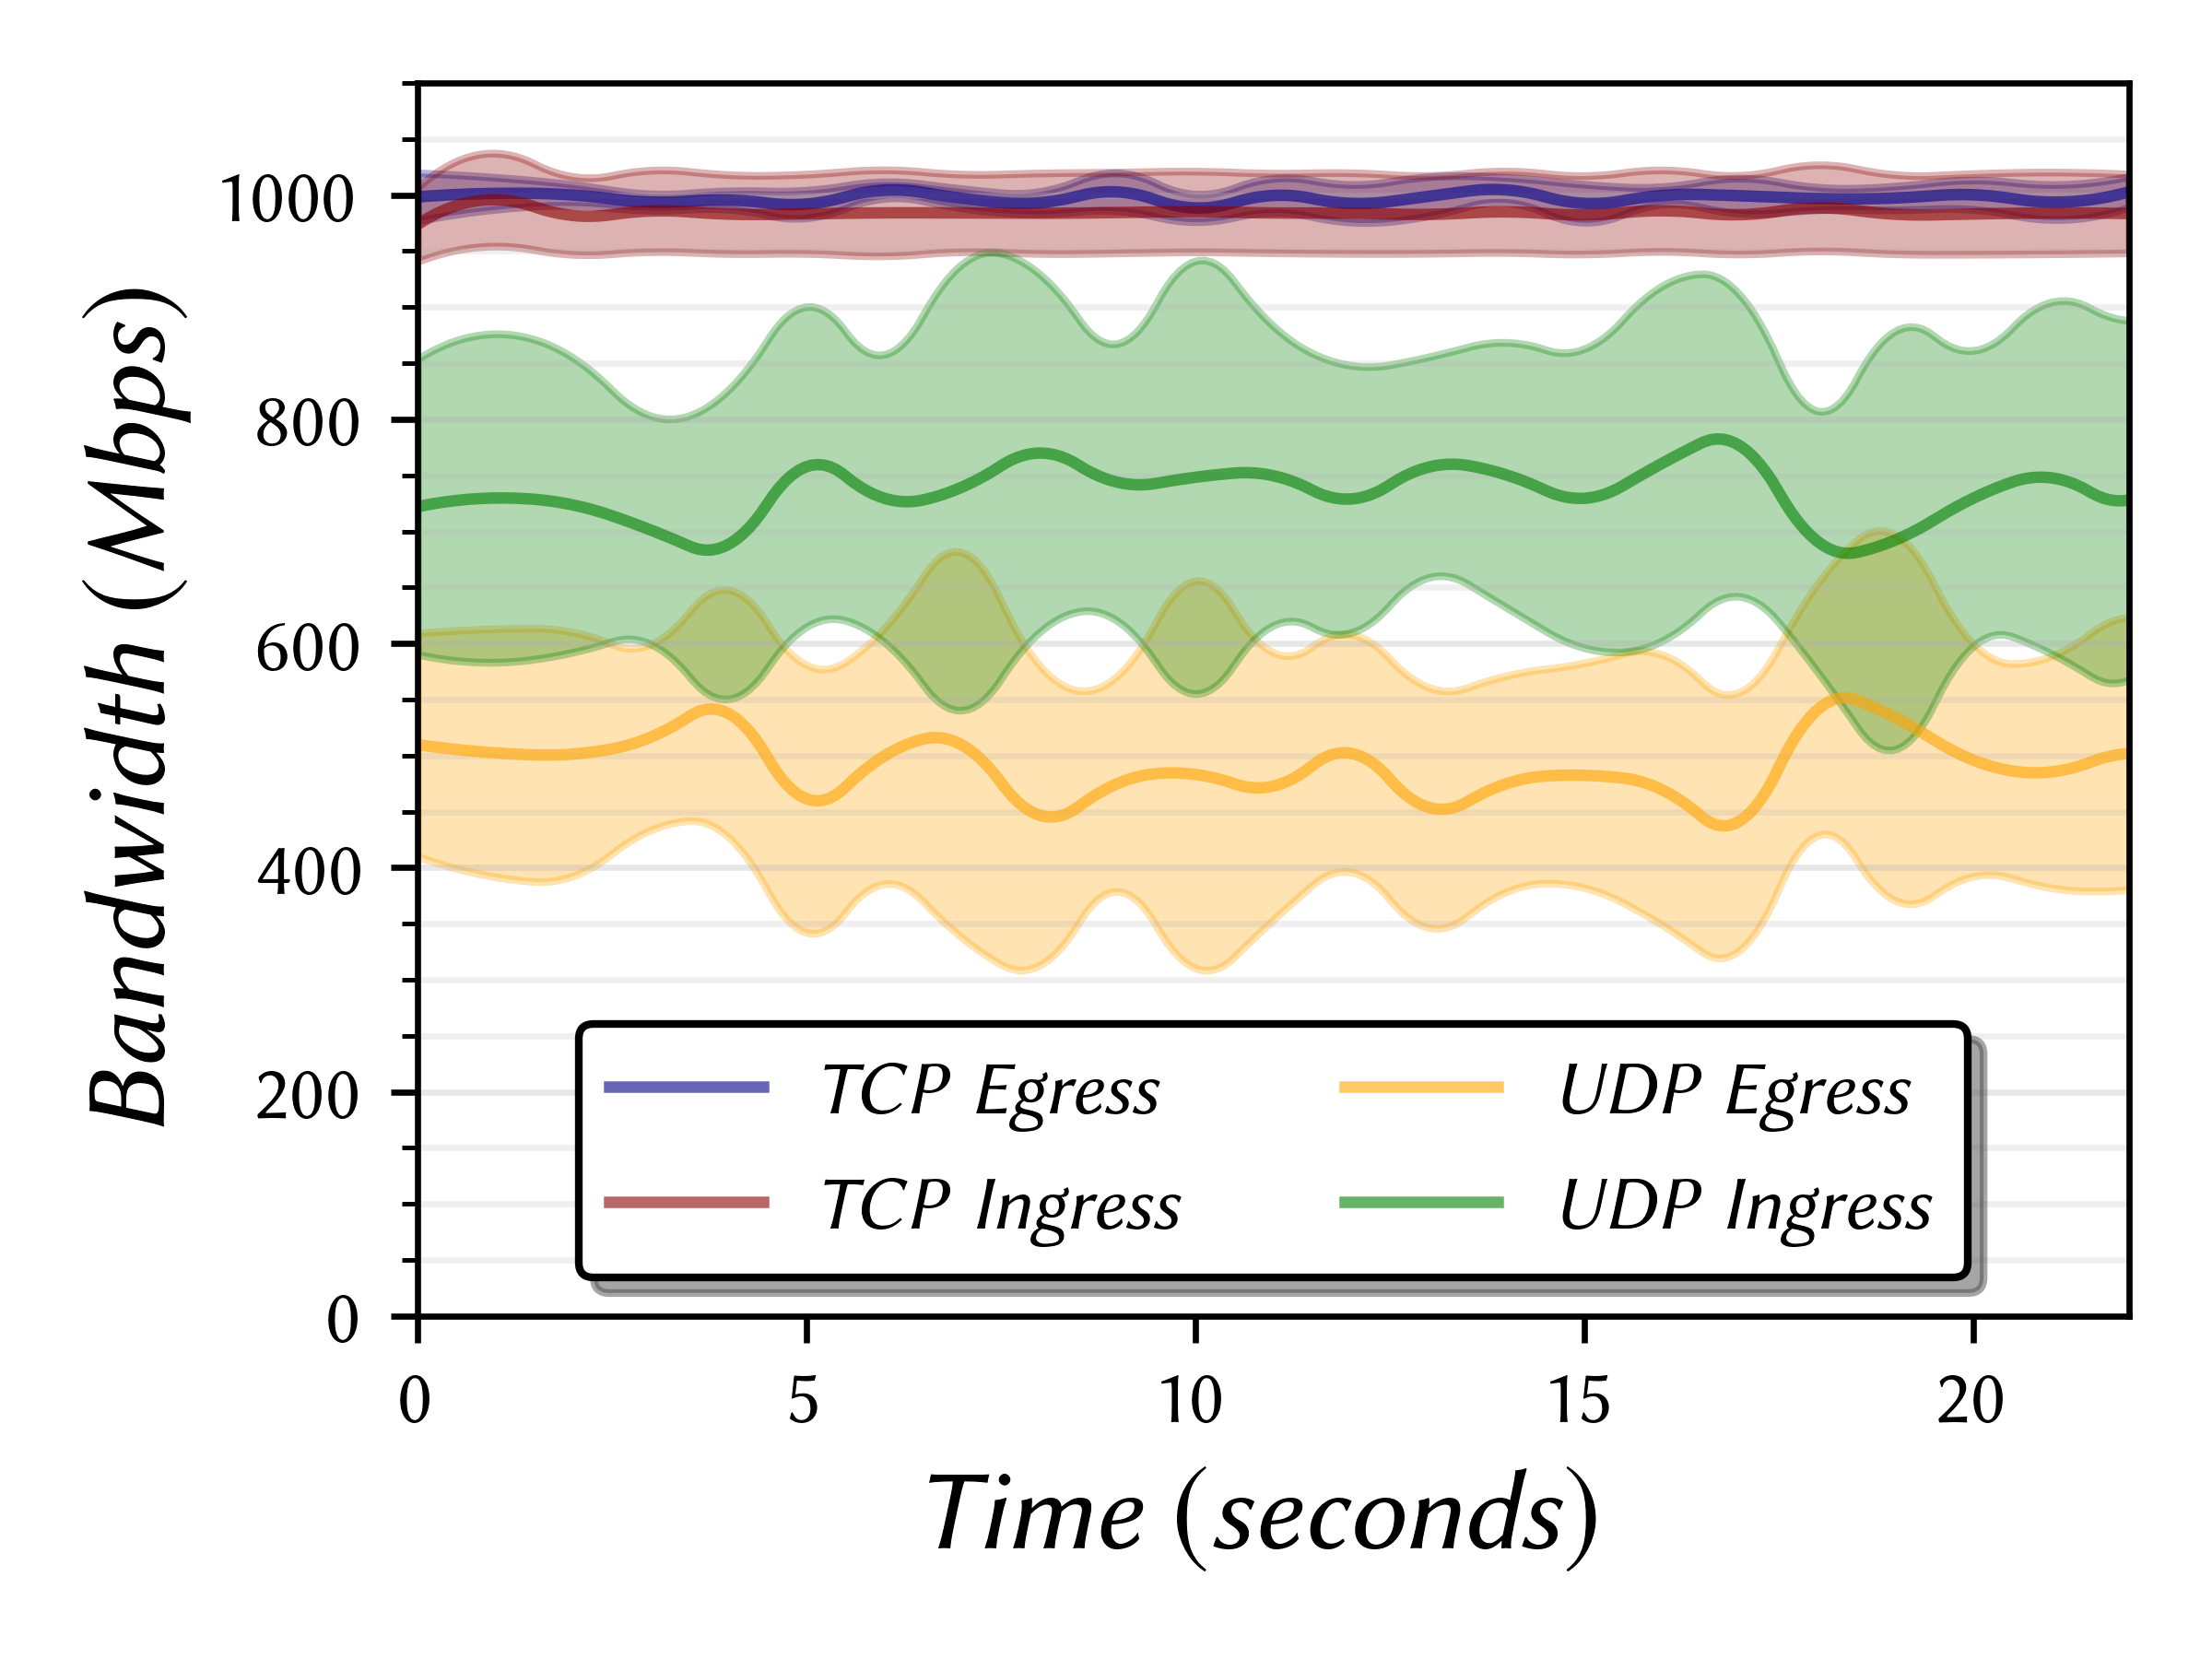
\includegraphics[width=\hsize]{figs/cluster1/setA/vis-5-vm2-combined.png}
  \caption{$vm2$}
  \label{fig:bw-bidir-1:c}
\end{subfigure}%

\medskip


\hfill%
\begin{subfigure}{.33\textwidth}
  \centering
  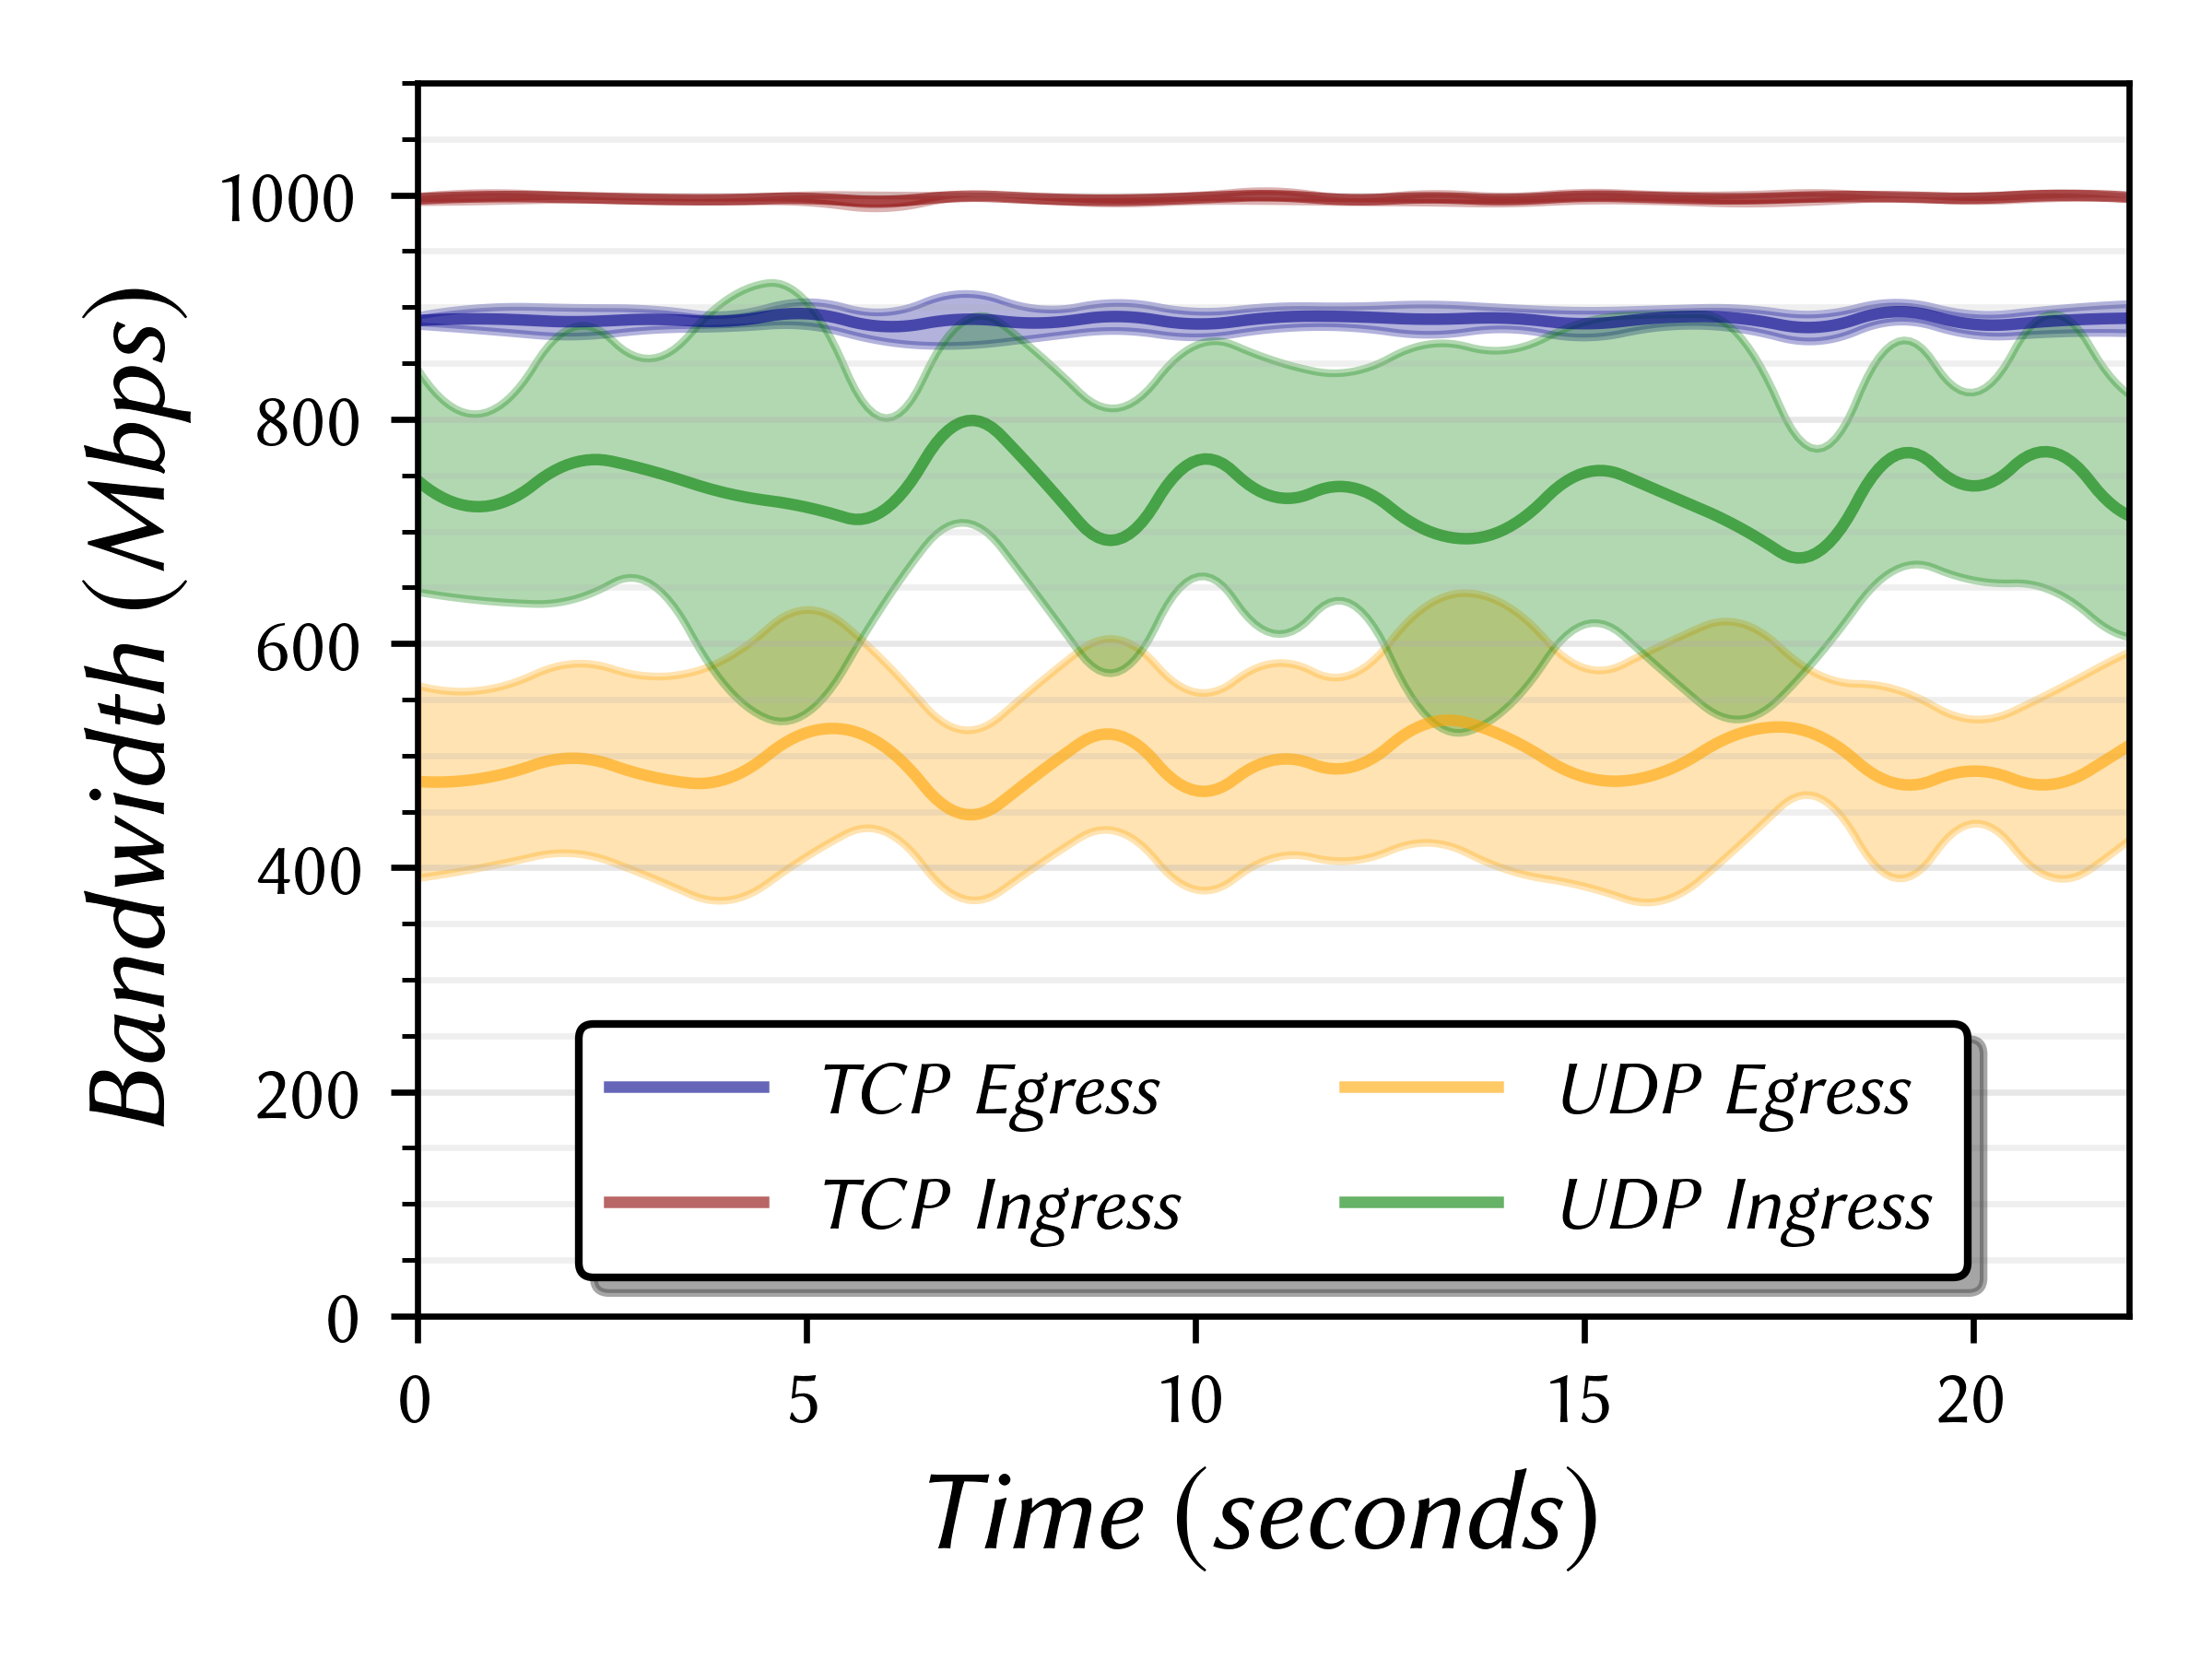
\includegraphics[width=\hsize]{figs/cluster1/setA/vis-5-vm3-combined.png}
  \caption{$vm3$}
  \label{fig:bw-bidir-1:d}
\end{subfigure}%
\begin{subfigure}{.33\textwidth}
  \centering
  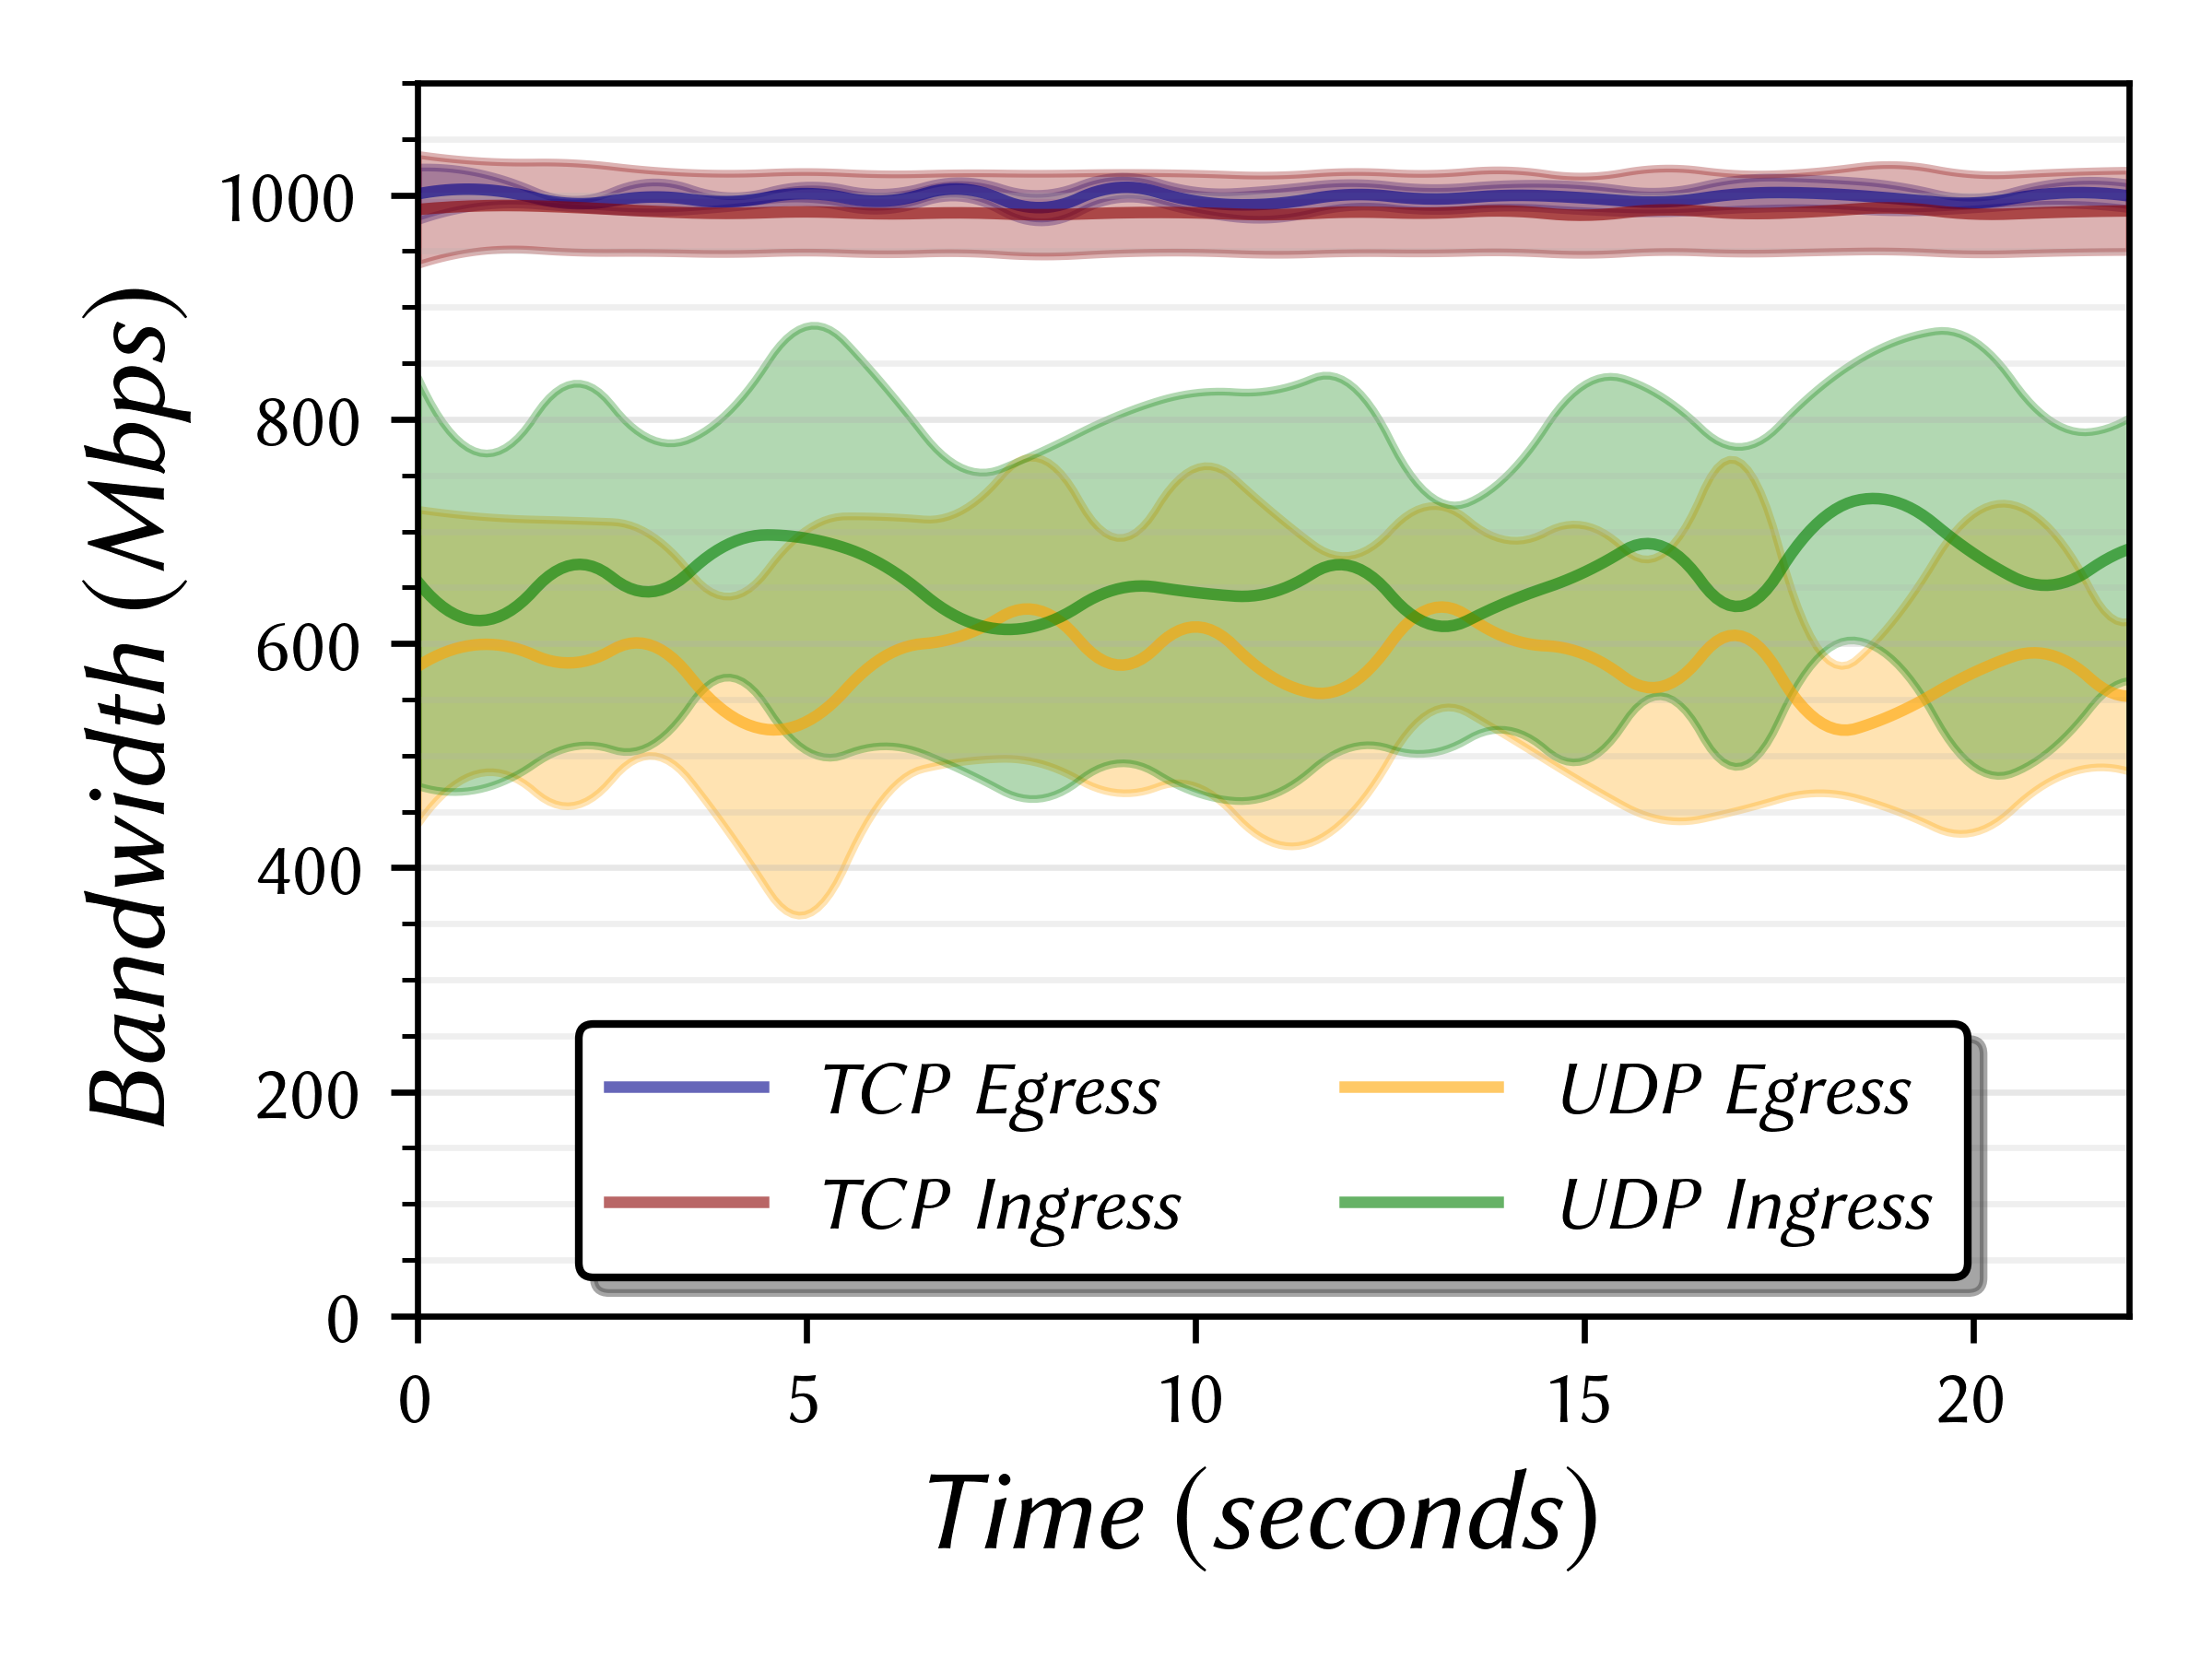
\includegraphics[width=\hsize]{figs/cluster1/setA/vis-5-vm4-combined.png}
  \caption{$vm4$}
  \label{fig:bw-bidir-1:e}
\end{subfigure}%
\hspace{0.17\textwidth}


\caption{\centering{} Cluster 1 VM \texttt{iperf} bidirectional bandwidth trials. \\ (The first 5 seconds are clipped to allow the network to settle, error bounds are $\pm s$, the sample std. dev.) \\ \texttt{cluster1/setA/d8}, Experiment 4 (Combined) }
\label{fig:bw-bidir-1}
\end{figure}

\begin{figure}
\centering
\begin{subfigure}{.33\textwidth}
  \centering
  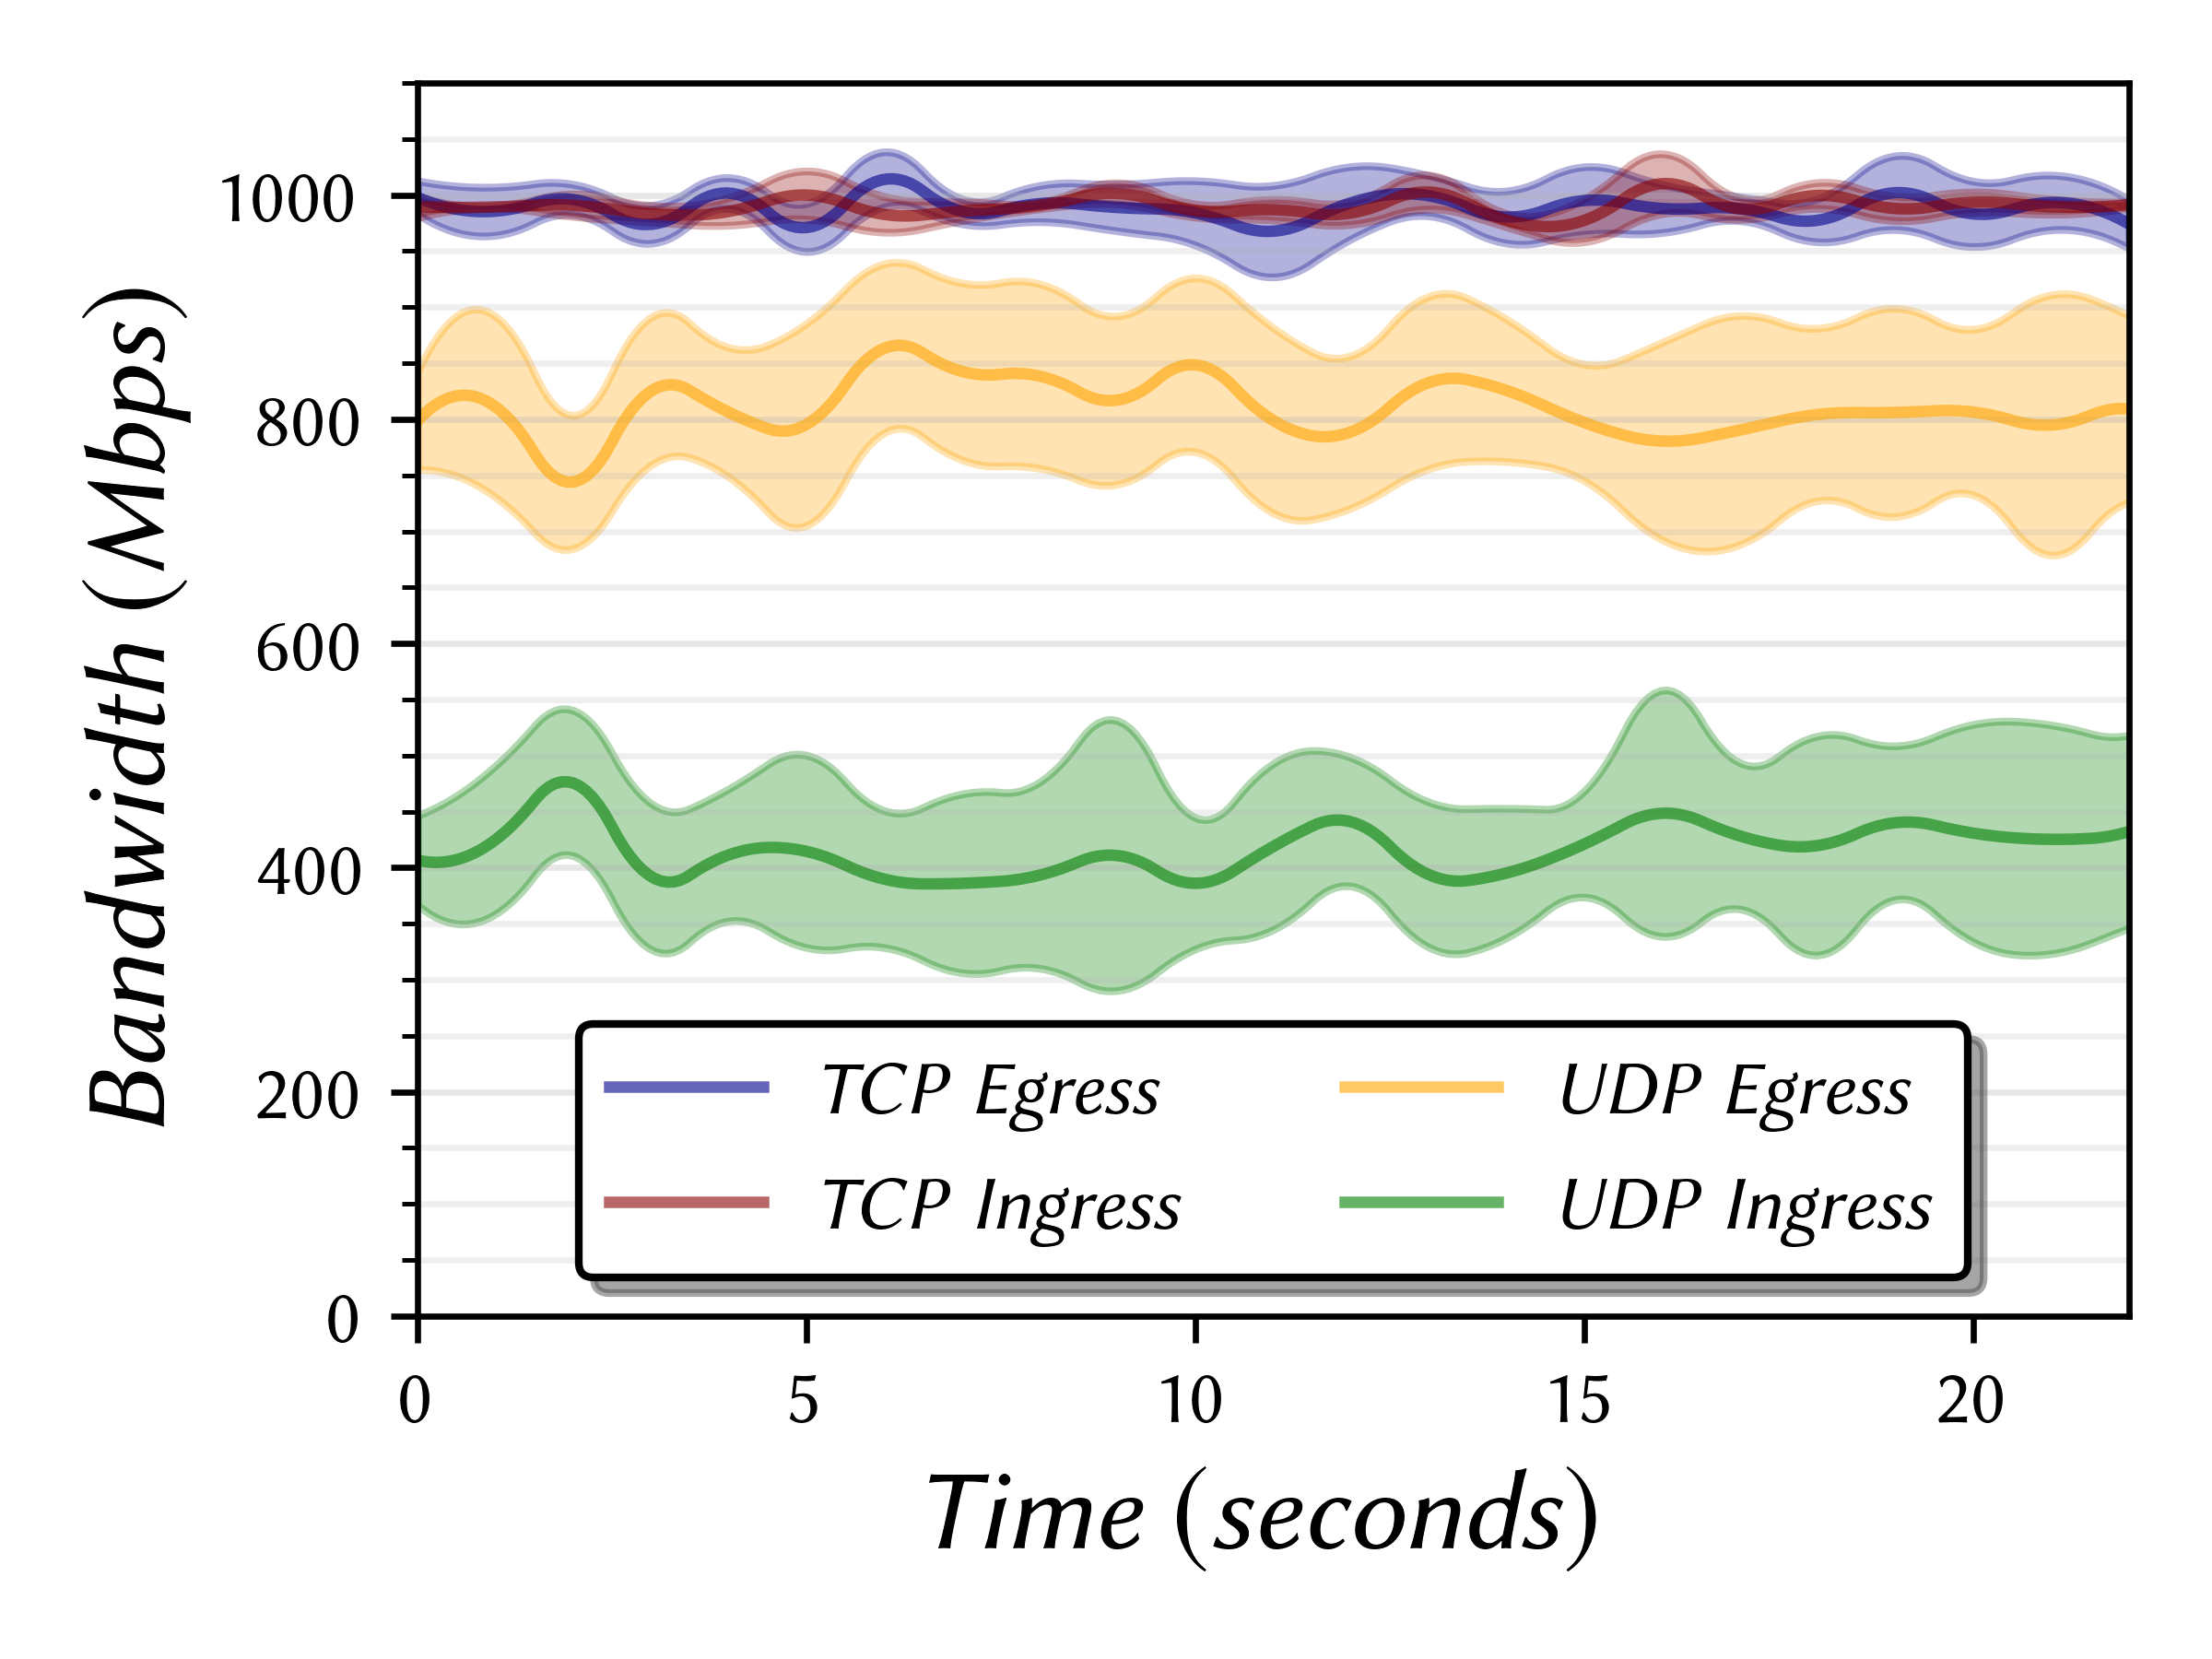
\includegraphics[width=\hsize]{figs/cluster2/setA/vis-5-vm0-combined.png}
  \caption{$vm0$}
  \label{fig:bw-bidir-2:a}
\end{subfigure}%
\hfill%
\begin{subfigure}{.33\textwidth}
  \centering
  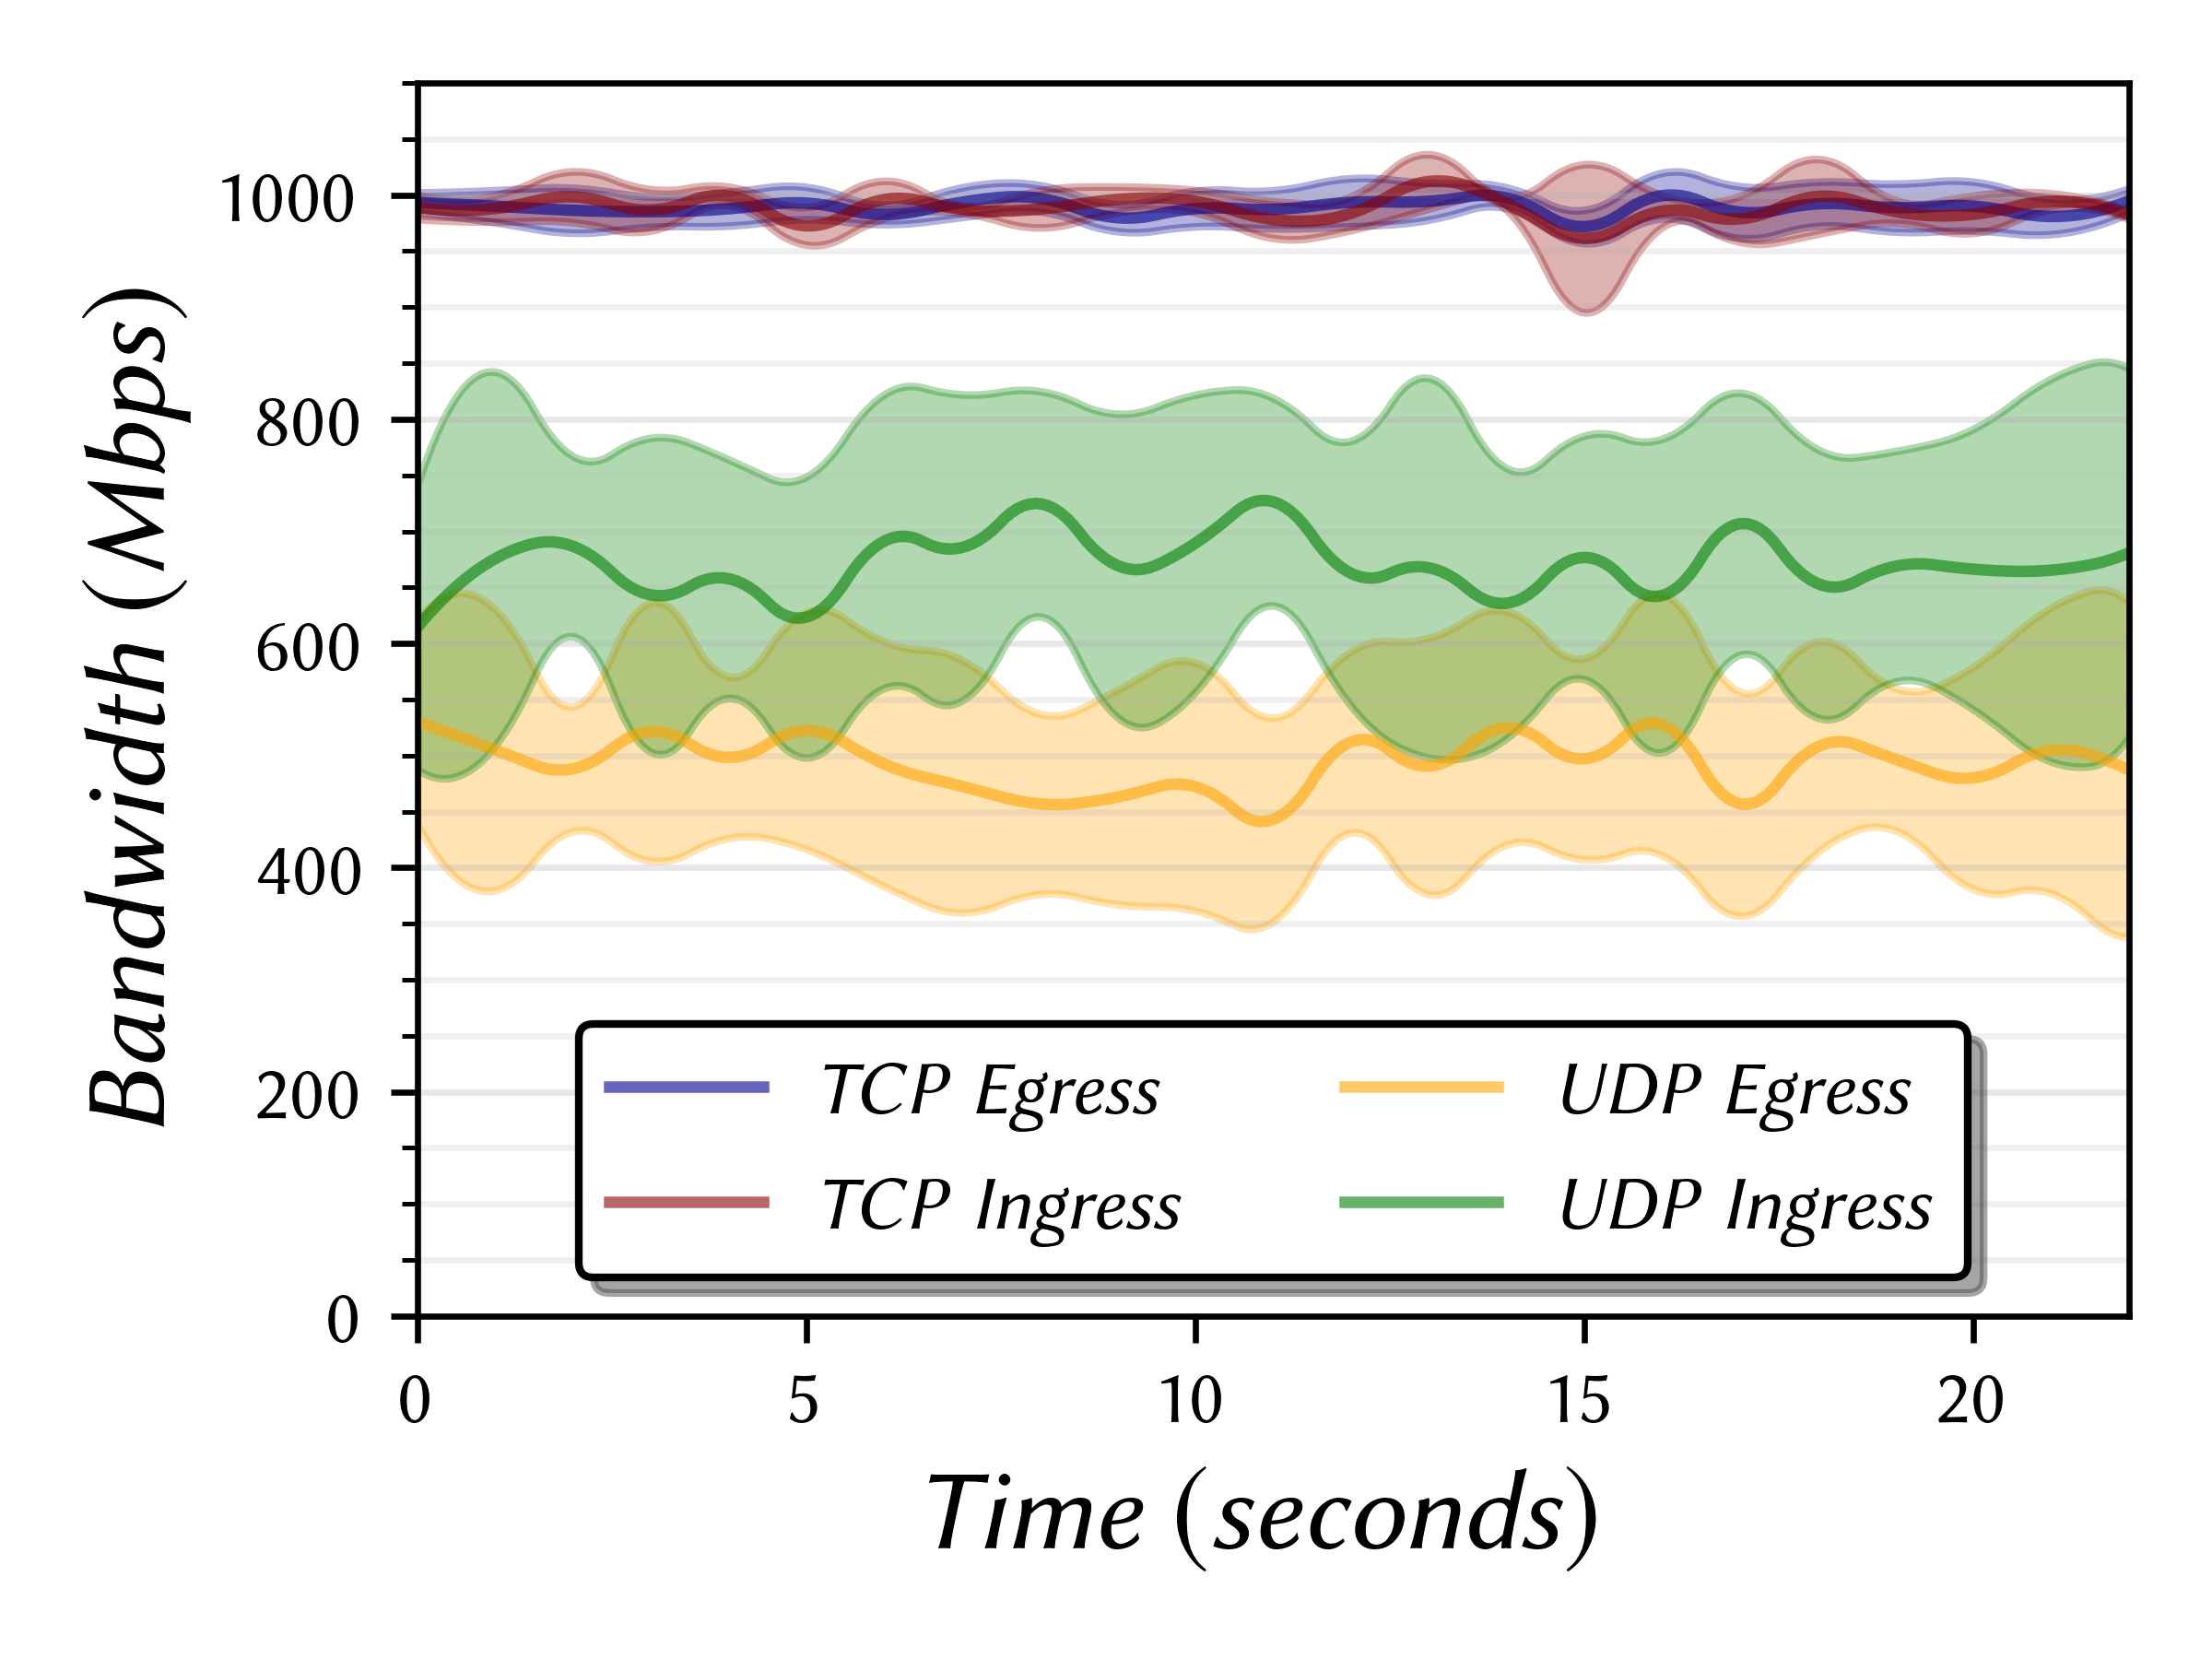
\includegraphics[width=\hsize]{figs/cluster2/setA/vis-5-vm1-combined.png}
  \caption{$vm1$}
  \label{fig:bw-bidir-2:b}
\end{subfigure}%
\hfill%
\begin{subfigure}{.33\textwidth}
  \centering
  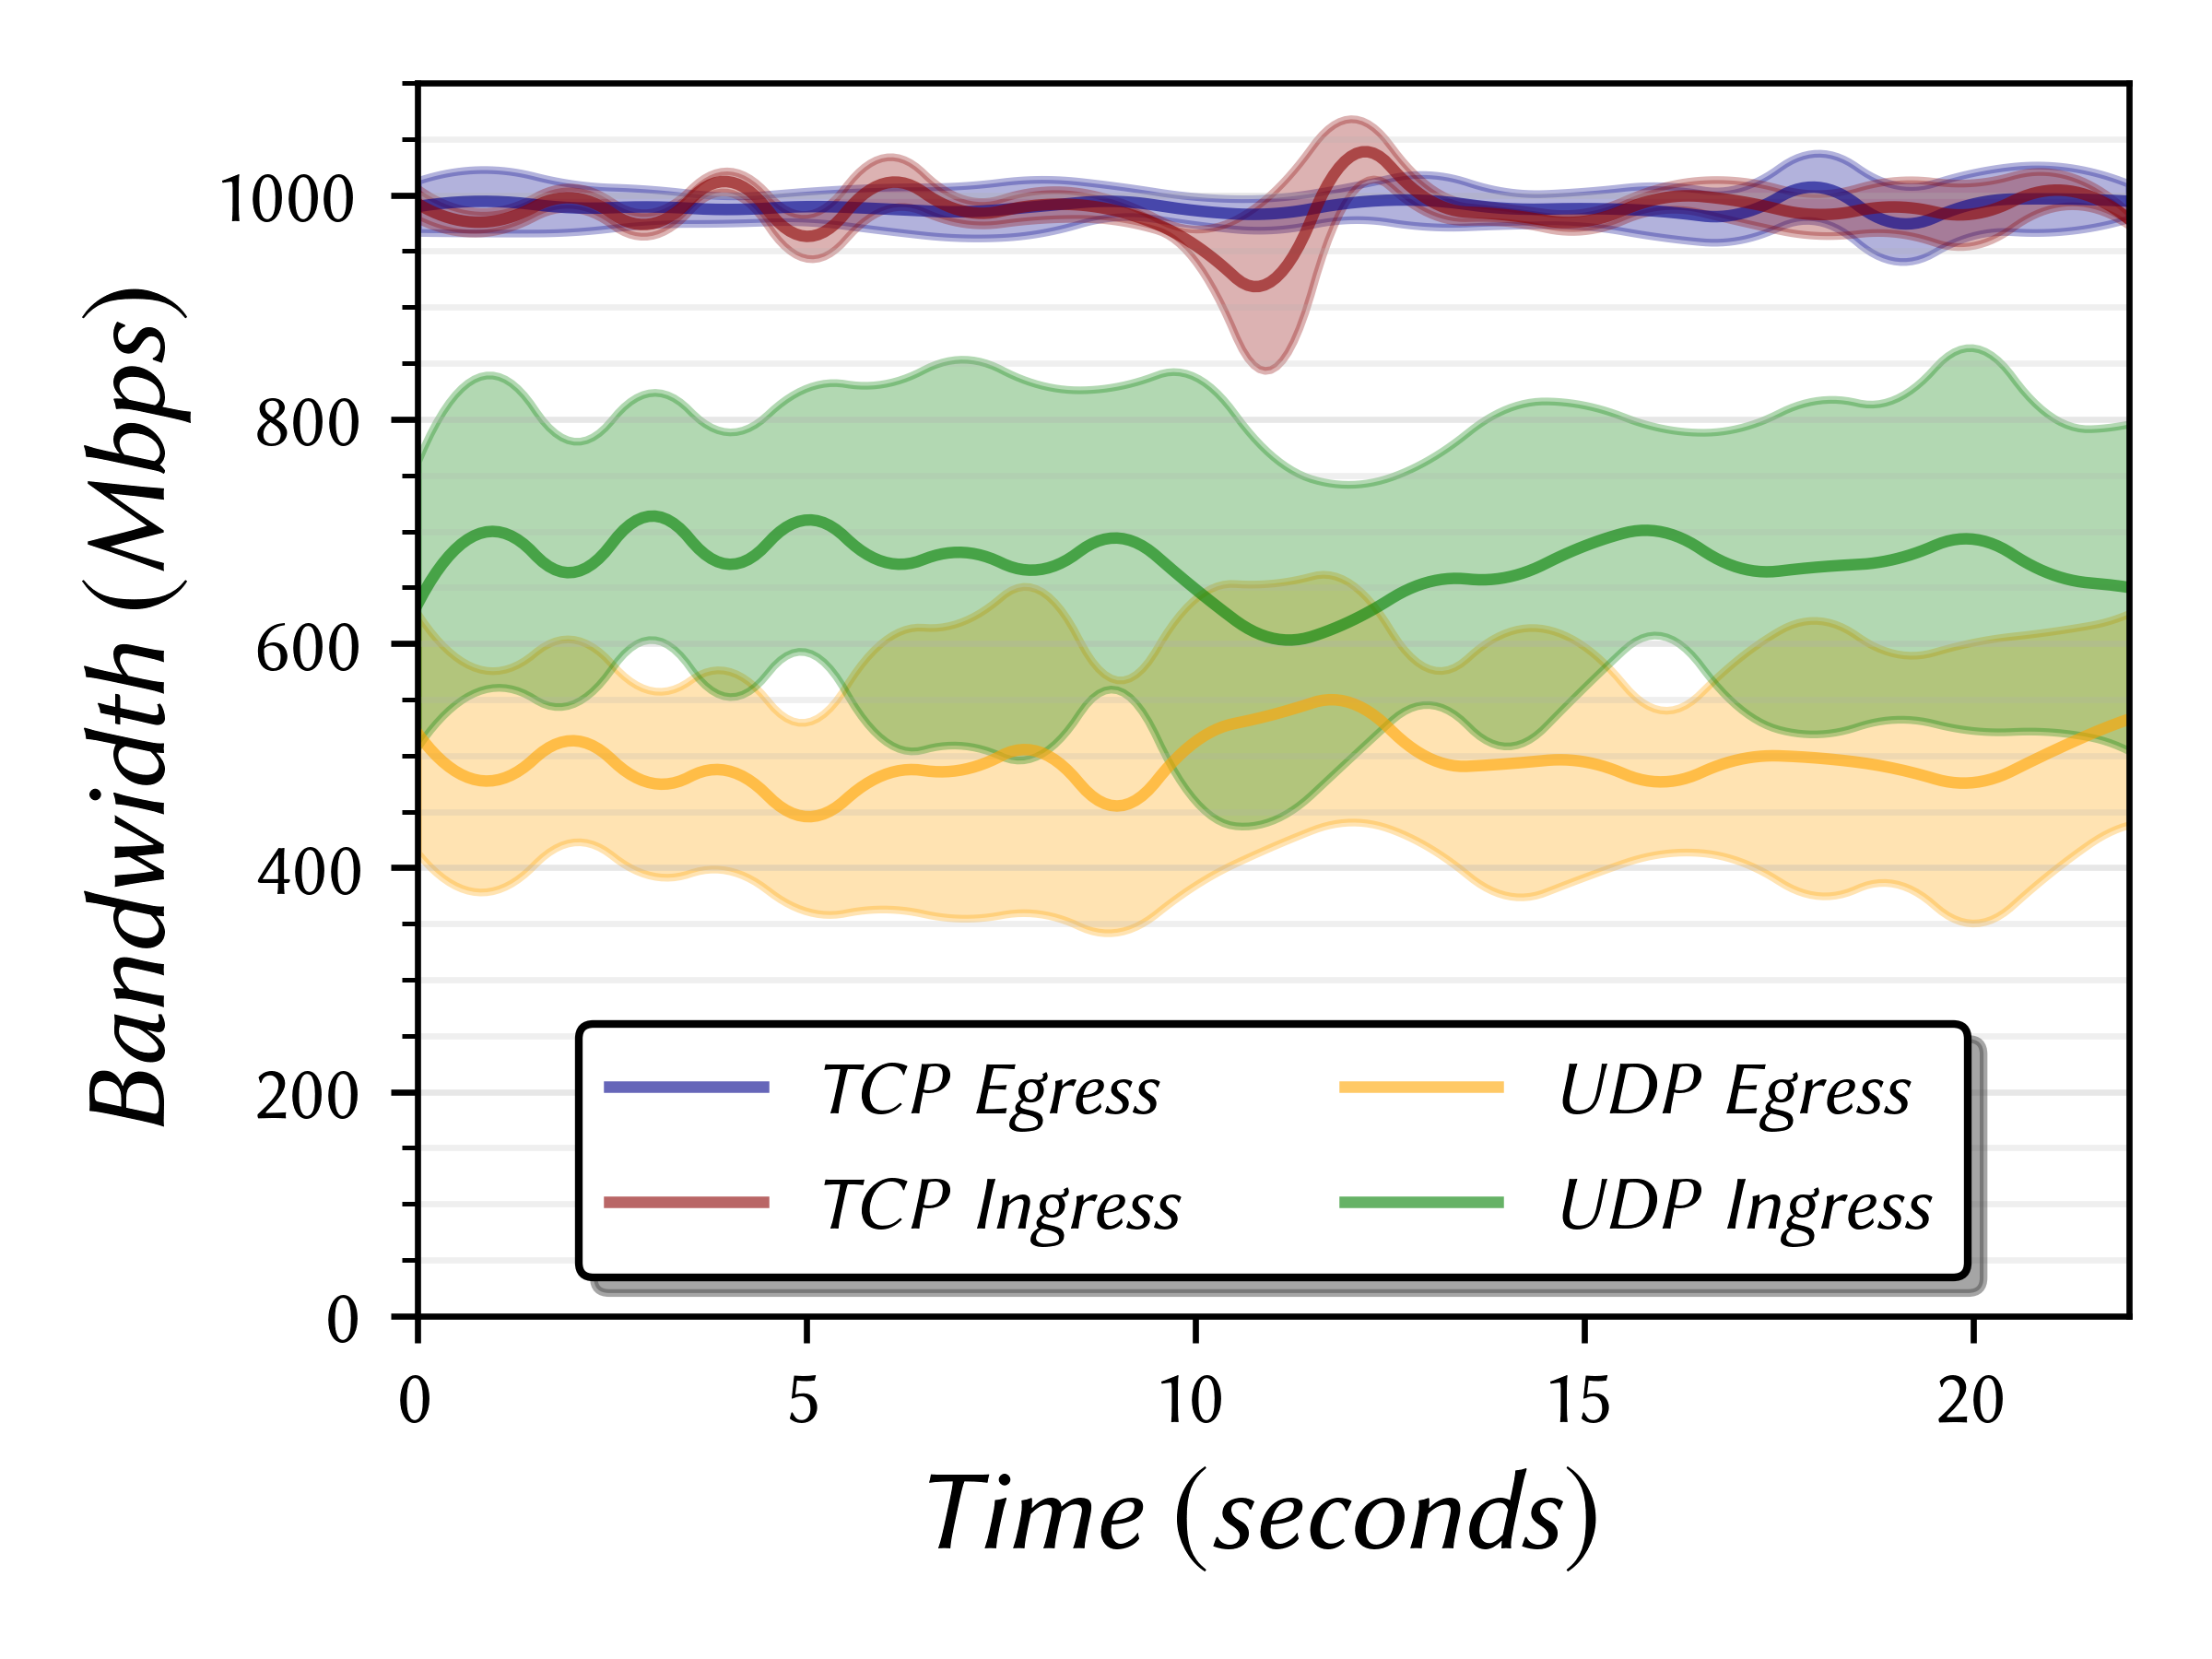
\includegraphics[width=\hsize]{figs/cluster2/setA/vis-5-vm2-combined.png}
  \caption{$vm2$}
  \label{fig:bw-bidir-2:c}
\end{subfigure}%

\medskip


\hfill%
\begin{subfigure}{.33\textwidth}
  \centering
  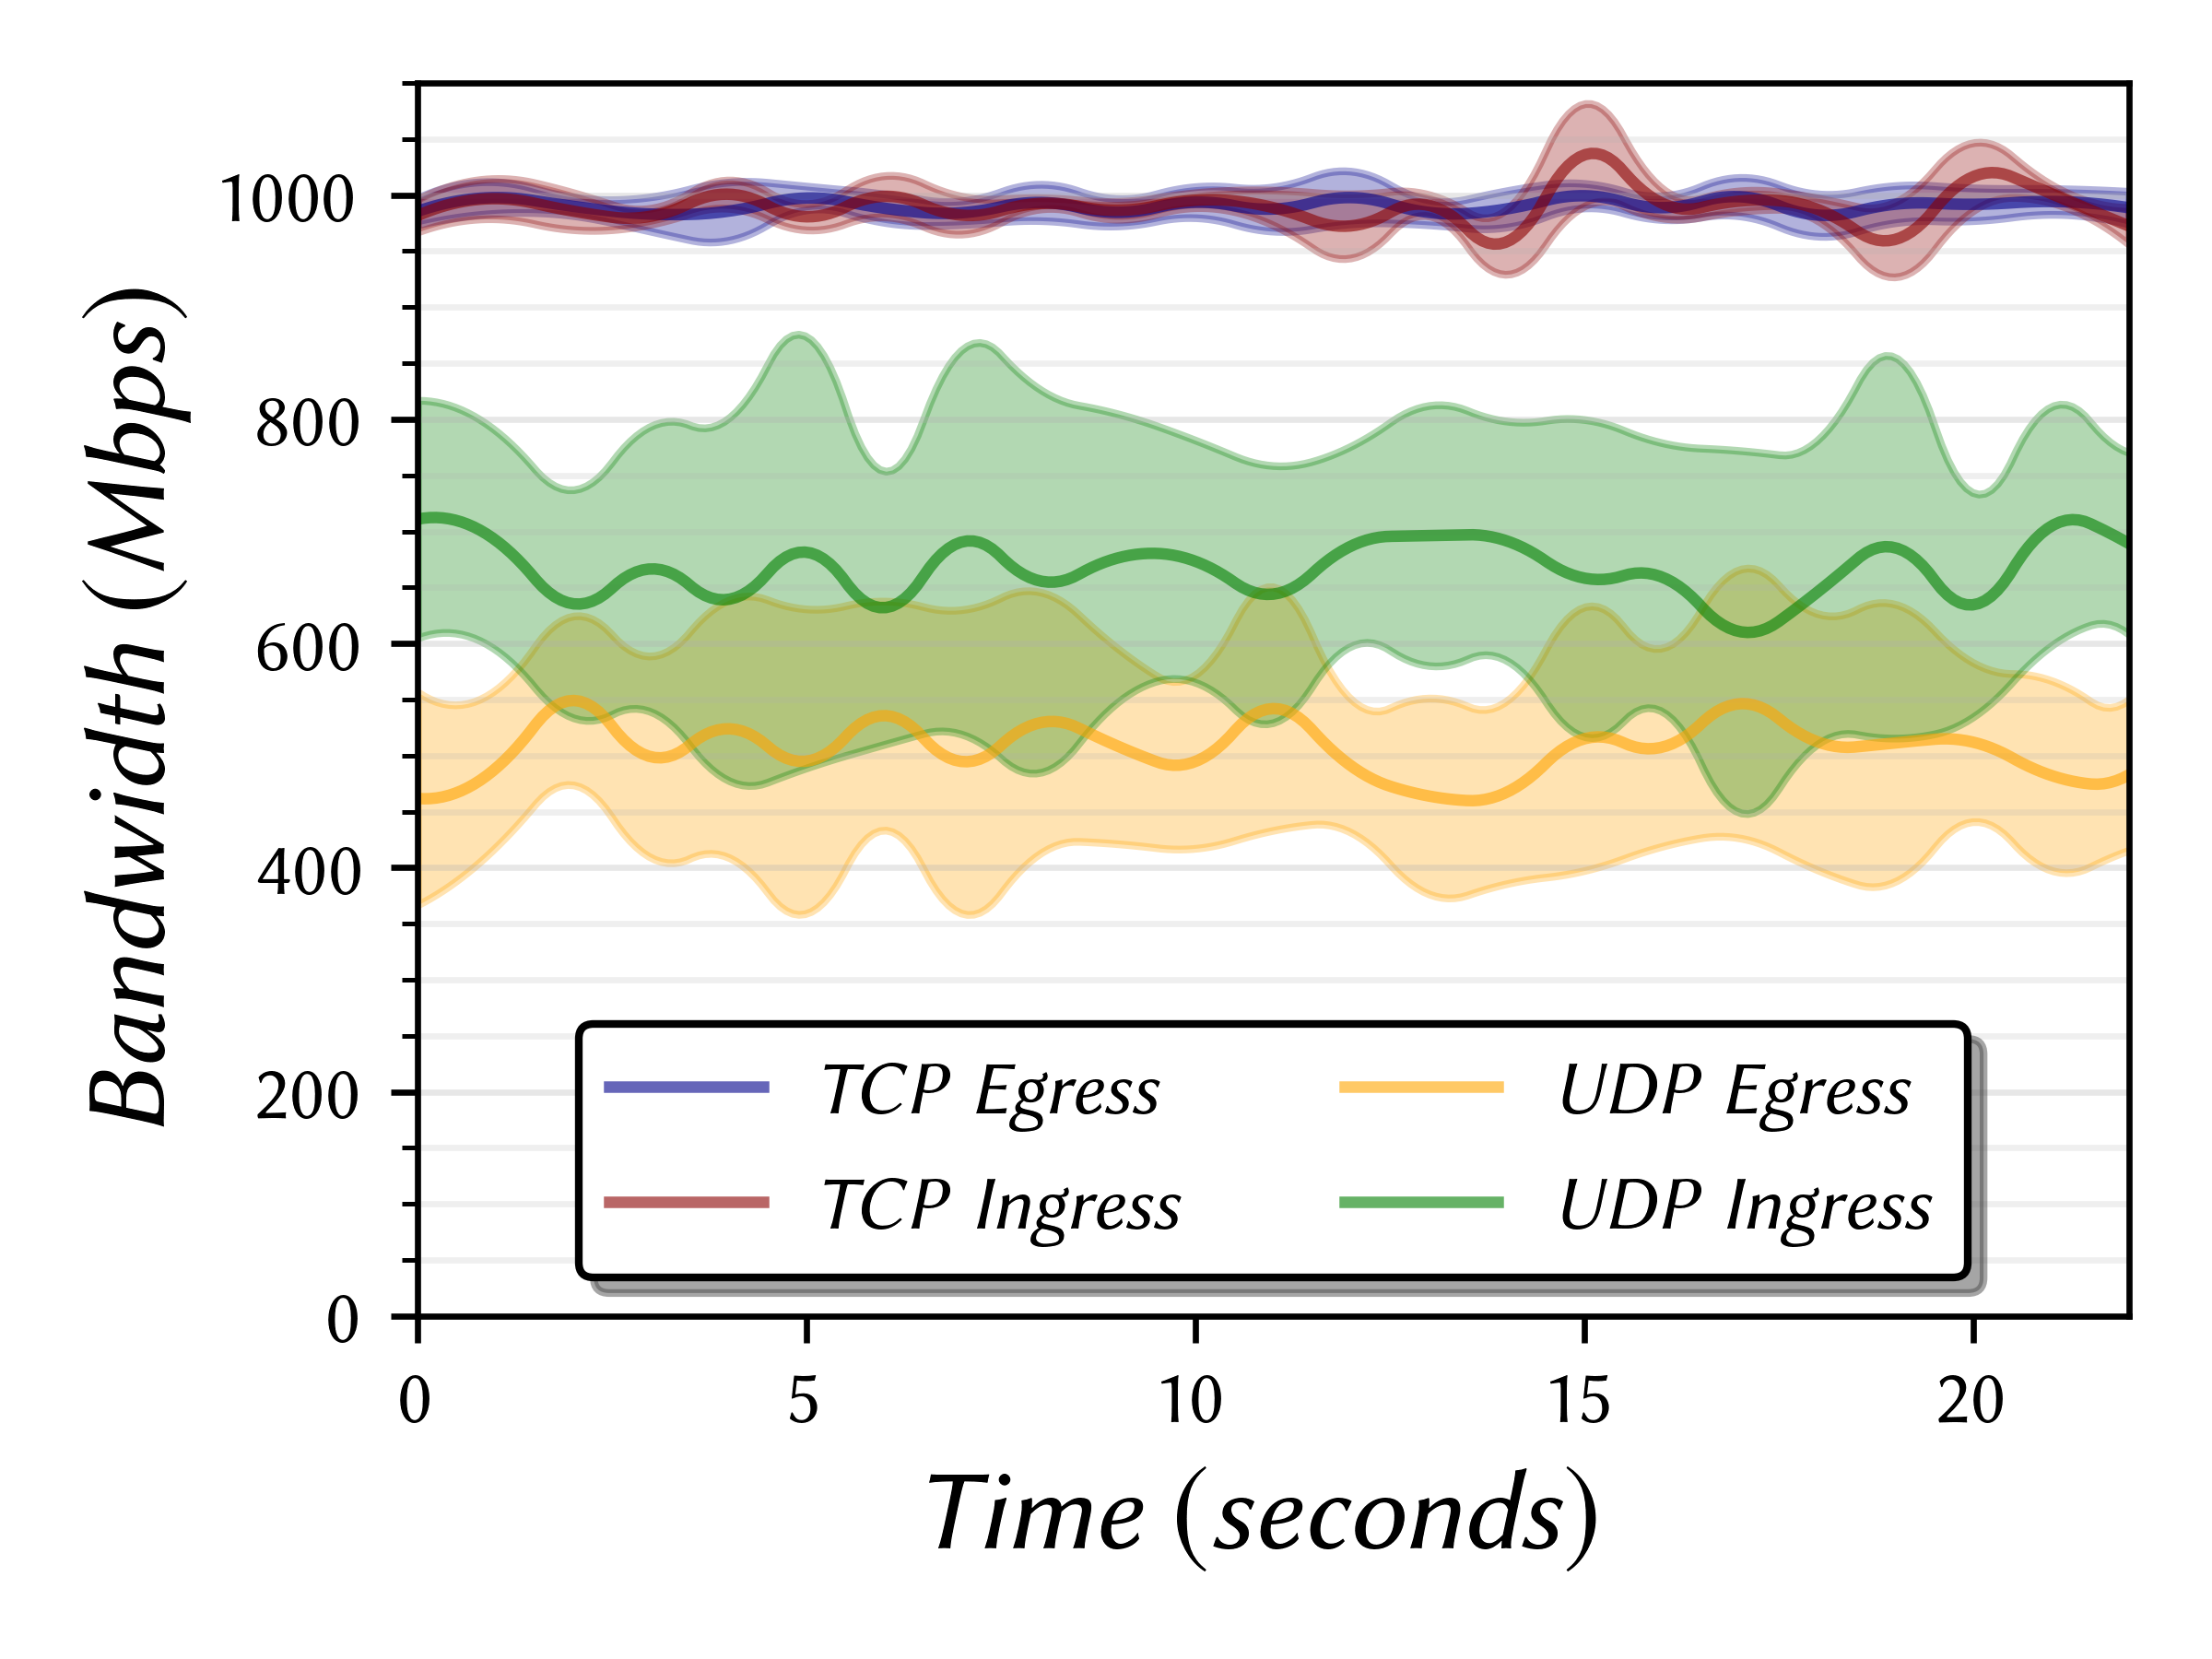
\includegraphics[width=\hsize]{figs/cluster2/setA/vis-5-vm3-combined.png}
  \caption{$vm3$}
  \label{fig:bw-bidir-2:d}
\end{subfigure}%
\begin{subfigure}{.33\textwidth}
  \centering
  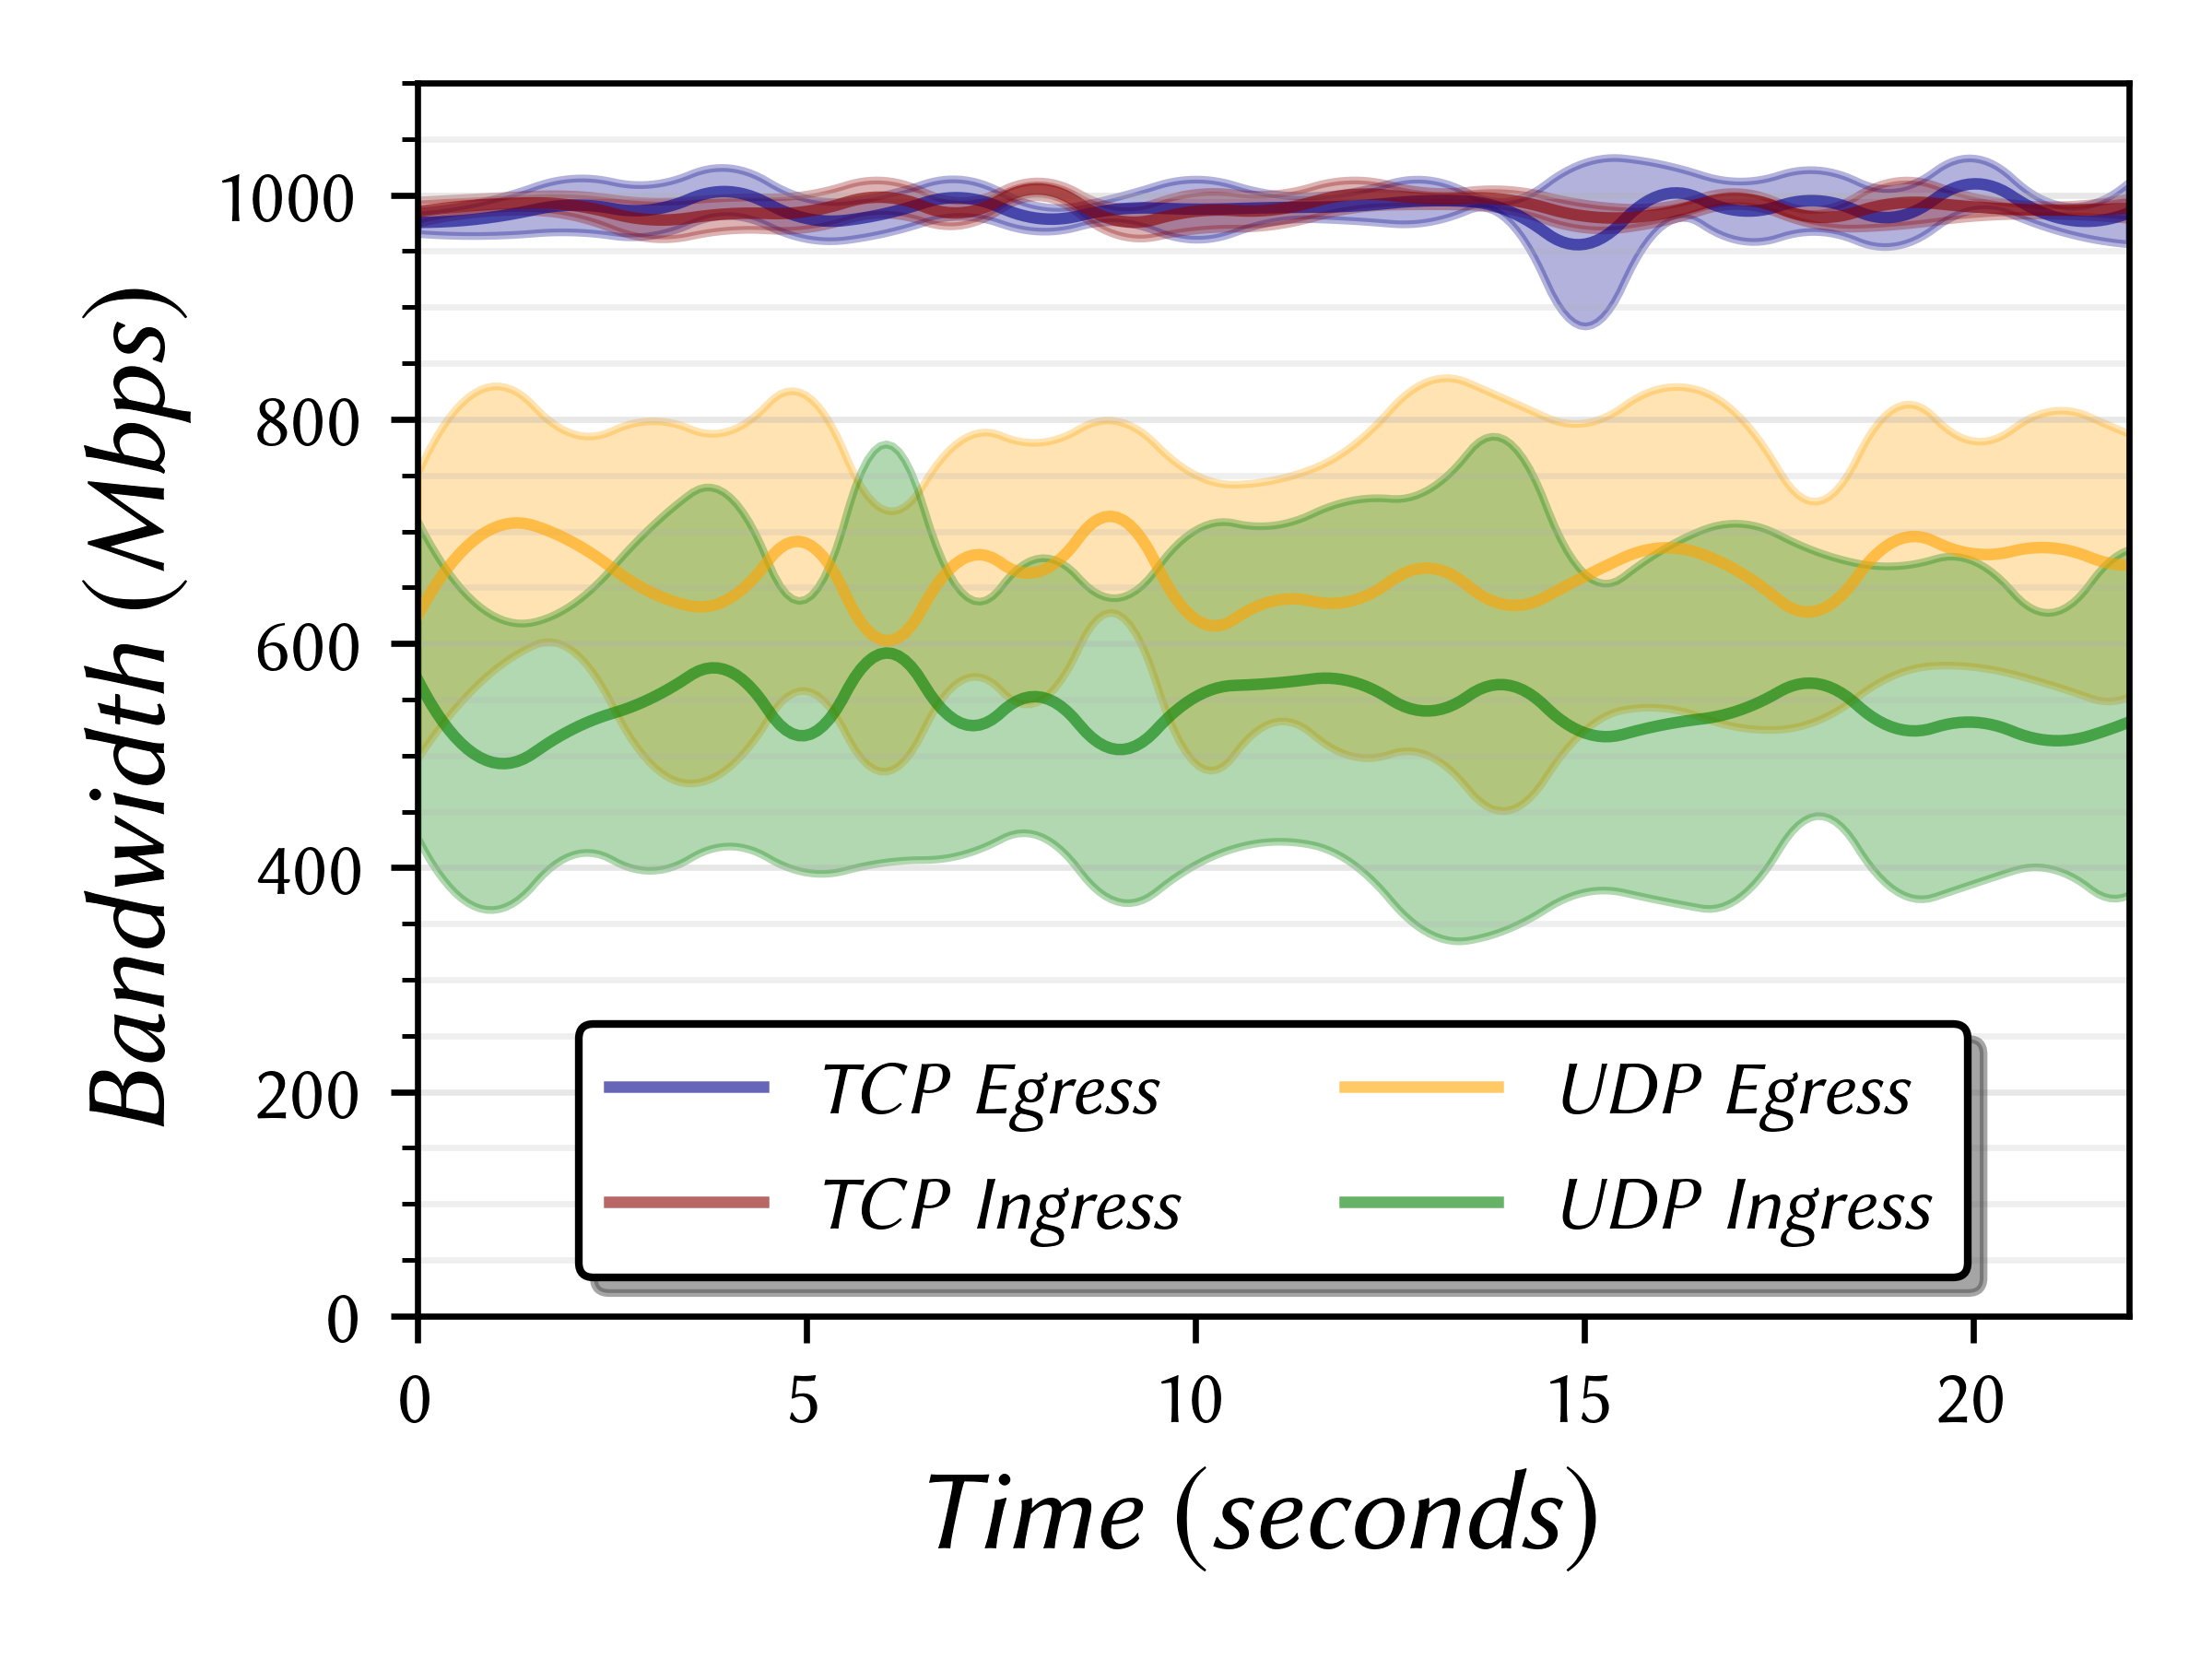
\includegraphics[width=\hsize]{figs/cluster2/setA/vis-5-vm4-combined.png}
  \caption{$vm4$}
  \label{fig:bw-bidir-2:e}
\end{subfigure}%
\hspace{0.17\textwidth}


\caption{\centering{} Cluster 2 VM \texttt{iperf} bidirectional bandwidth trials. \\ (The first 5 seconds are clipped to allow the network to settle, error bounds are $\pm s$, the sample std. dev.) \\ \texttt{cluster2/setA/d8}, Experiment 4 (Combined) }
\label{fig:bw-bidir-2}
\end{figure}

\clearpage

\begin{figure}
\centering

\foreach \hostnumber in {0,1,2,3,4}{
    \foreach \imagenumber in {1,2,3,4}{
        % \imagenumber --- \hostnumber
        \begin{subfigure}{.24\textwidth}
          \centering
          \includegraphics[width=\hsize]{figs/cluster1/setA/aggr-vis-8-vm\hostnumber-\imagenumber.png}
          \vspace{-7mm}
          \caption{$vm\hostnumber{}$, \imagenumber{} Gbps ingress}
        \end{subfigure}%
    }
    \medskip
}
\caption{\centering{} Cluster 1 \texttt{iperf3} maximum ingress trials \\ \texttt{cluster1/setA/aggr}, Experiment 5 \\ The first 5 seconds are clipped to allow the network to settle, error bounds are $\pm s$, the sample std. dev. \\ {[Blue is the total received bandwidth, Green and Red are the per-sender bandwidths received and sent]}}
\label{fig:bw-n-1-1}
\end{figure}

\clearpage


\begin{figure}
\centering

\foreach \hostnumber in {0,1,2,3,4}{
    \foreach \imagenumber in {1,2,3,4}{
        % \imagenumber --- \hostnumber
        \begin{subfigure}{.24\textwidth}
          \centering
          \includegraphics[width=\hsize]{figs/cluster2/setA/aggr-vis-8-vm\hostnumber-\imagenumber.png}
          \vspace{-5mm}
          \caption{$vm\hostnumber{}$, \imagenumber{} Gbps ingress}
        \end{subfigure}%
    }
    \smskip
}
\caption{\centering{} Cluster 2 \texttt{iperf3} maximum ingress trials \\ \texttt{cluster2/setA/aggr}, Experiment 5 \\ The first 5 seconds are clipped to allow the network to settle, error bounds are $\pm s$, the sample std. dev.) \\ {[Blue is the total received bandwidth, Green and Red are the per-sender bandwidths received and sent]}}
\label{fig:bw-n-1-2}
\end{figure}

\clearpage

\begin{figure}
\centering

\foreach \hostnumber in {0,1,2,3,4}{
    \foreach \imagenumber in {1,2,3,4}{
        % \imagenumber --- \hostnumber
        \begin{subfigure}{.24\textwidth}
          \centering
          \includegraphics[width=\hsize]{figs/cluster1/setA/aggr-vis-9-vm\hostnumber-\imagenumber.png}
          \vspace{-5mm}
          \caption{$vm\hostnumber{}$, \imagenumber{} \texttt{iperf} instances}
        \end{subfigure}%
    }
    \smskip
}
\caption{\centering{} Cluster 1 \texttt{iperf3} maximum multi-flow egress trials \\ \texttt{cluster1/setA/aggr}, Experiment 6 \\ The first 5 seconds are clipped to allow the network to settle, error bounds are $\pm s$, the sample std. dev.) \\ {[Red is the total egress bandwidth, Green the per-process observed egress]}}
\label{fig:bw-1-n-1}
\end{figure}

\begin{figure}
\centering

\foreach \hostnumber in {0,1,2,3,4}{
    \foreach \imagenumber in {1,2,3,4}{
        % \imagenumber --- \hostnumber
        \begin{subfigure}{.24\textwidth}
          \centering
          \includegraphics[width=\hsize]{figs/cluster2/setA/aggr-vis-9-vm\hostnumber-\imagenumber.png}
          \vspace{-5mm}
          \caption{$vm\hostnumber{}$, \imagenumber{} \texttt{iperf} instances}
        \end{subfigure}%
    }
    \smskip
}
\caption{\centering{} Cluster 2 \texttt{iperf3} maximum multi-flow egress trials \\ \texttt{cluster2/setA/aggr}, Experiment 6 \\ The first 5 seconds are clipped to allow the network to settle, error bounds are $\pm s$, the sample std. dev.) \\ {[Red is the total egress bandwidth, Green the per-process observed egress]}}
\label{fig:bw-1-n-2}
\end{figure}

\clearpage
\section{Further Experimentation}

\paragraph{} The evaluation presented in the report will also consider two extensions beyond the basic latency and bandwidth trials presented in §~\ref{sec:latency} and §~\ref{sec:bandwidth};

\begin{enumerate}
    \item \textbf{Crosstalk} --- all of the experiments presented are implicitly measuring behaviours in the cluster's VPN. This is a shared resource, and thus, to accurately simulate real-world shared-networking conditions, the network needs to be subjected to load other than that produced by the experiments.
    \item \textbf{Temporal Differences} --- nothing ever remains the same forever, and this is especially true in virtualised environments such as this. Microsoft will move VMs around their physical hardware, thus potentially affecting the performance observed from them --- whenever a VM is turned off via the web interface Azure moves it into a \textit{deallocated} state; this signifies it has been decoupled from the hardware it had been running on, and floats until reassigned to a new physical node.
\end{enumerate}

\subsection*{Crosstalk}
\paragraph{} The evaluation framework is able to very cheaply synthesise crosstalk in the cluster's network for the vast majority of experiments. There are few scenarios in which the framework is driving all VMs at the same time; predominantly it only drives two simultaneously, with the exceptions being Experiments 5 and 6. For Experiments 1 to 4, before any individual run starts the framework can choose to select two of the idle VMs and saturate the link between them using \texttt{iperf}. Whenever a full experiment run is being done, the framework runs the complete set of crosstalk-compatible experiments twice, one with and one without crosstalk enabled. In the data files this is marked with the \texttt{-crosstalk} prefix.

\paragraph{} Slightly disappointingly, crosstalk appears to have had no effect on the results at all. This logically makes sense, as the network does not actually physcially exists, it is entirely virtualised. Thus, simulating traffic between $vm0 \leftrightarrow vm1$ will likely use an entirely different set of physical resources to communication between $vm2 \leftrightarrow vm3$. For more information all the graphs are provided alongside their non-crosstalk counterparts in the accompanying data archive.

\subsection*{Temporal Differences}


\paragraph{} Provided alongside this report is four collections of recordings, 2 per cluster (\texttt{setA} and \texttt{setB}). Each collection contains 8 recordings (labelled \texttt{d\{1..8\}}), all done sequentially, triggered every 4 hours. In between \texttt{setA} and \texttt{setB} the clusters were deallocated and left for two days --- the purpose of this is to encourage any warm-standby copies of the VMs to expire, forcing the hypervisor to load their contents from cold storage at the start of \texttt{setB}. This is desirable as we want to break out of any sense of residence-locality brought by latent standby copies to maximise the chance of seeing drastic change in the behaviour of the clusters' reallocated VMs.

\paragraph{} The differences between \texttt{setA} and \texttt{setB} for both clusters is quite surprising. In the remainder of this section I will present the most striking differences seen across all experiments for both clusters.

\begin{figure}
    \centering
    \begin{subfigure}{.45\textwidth}
      \centering
      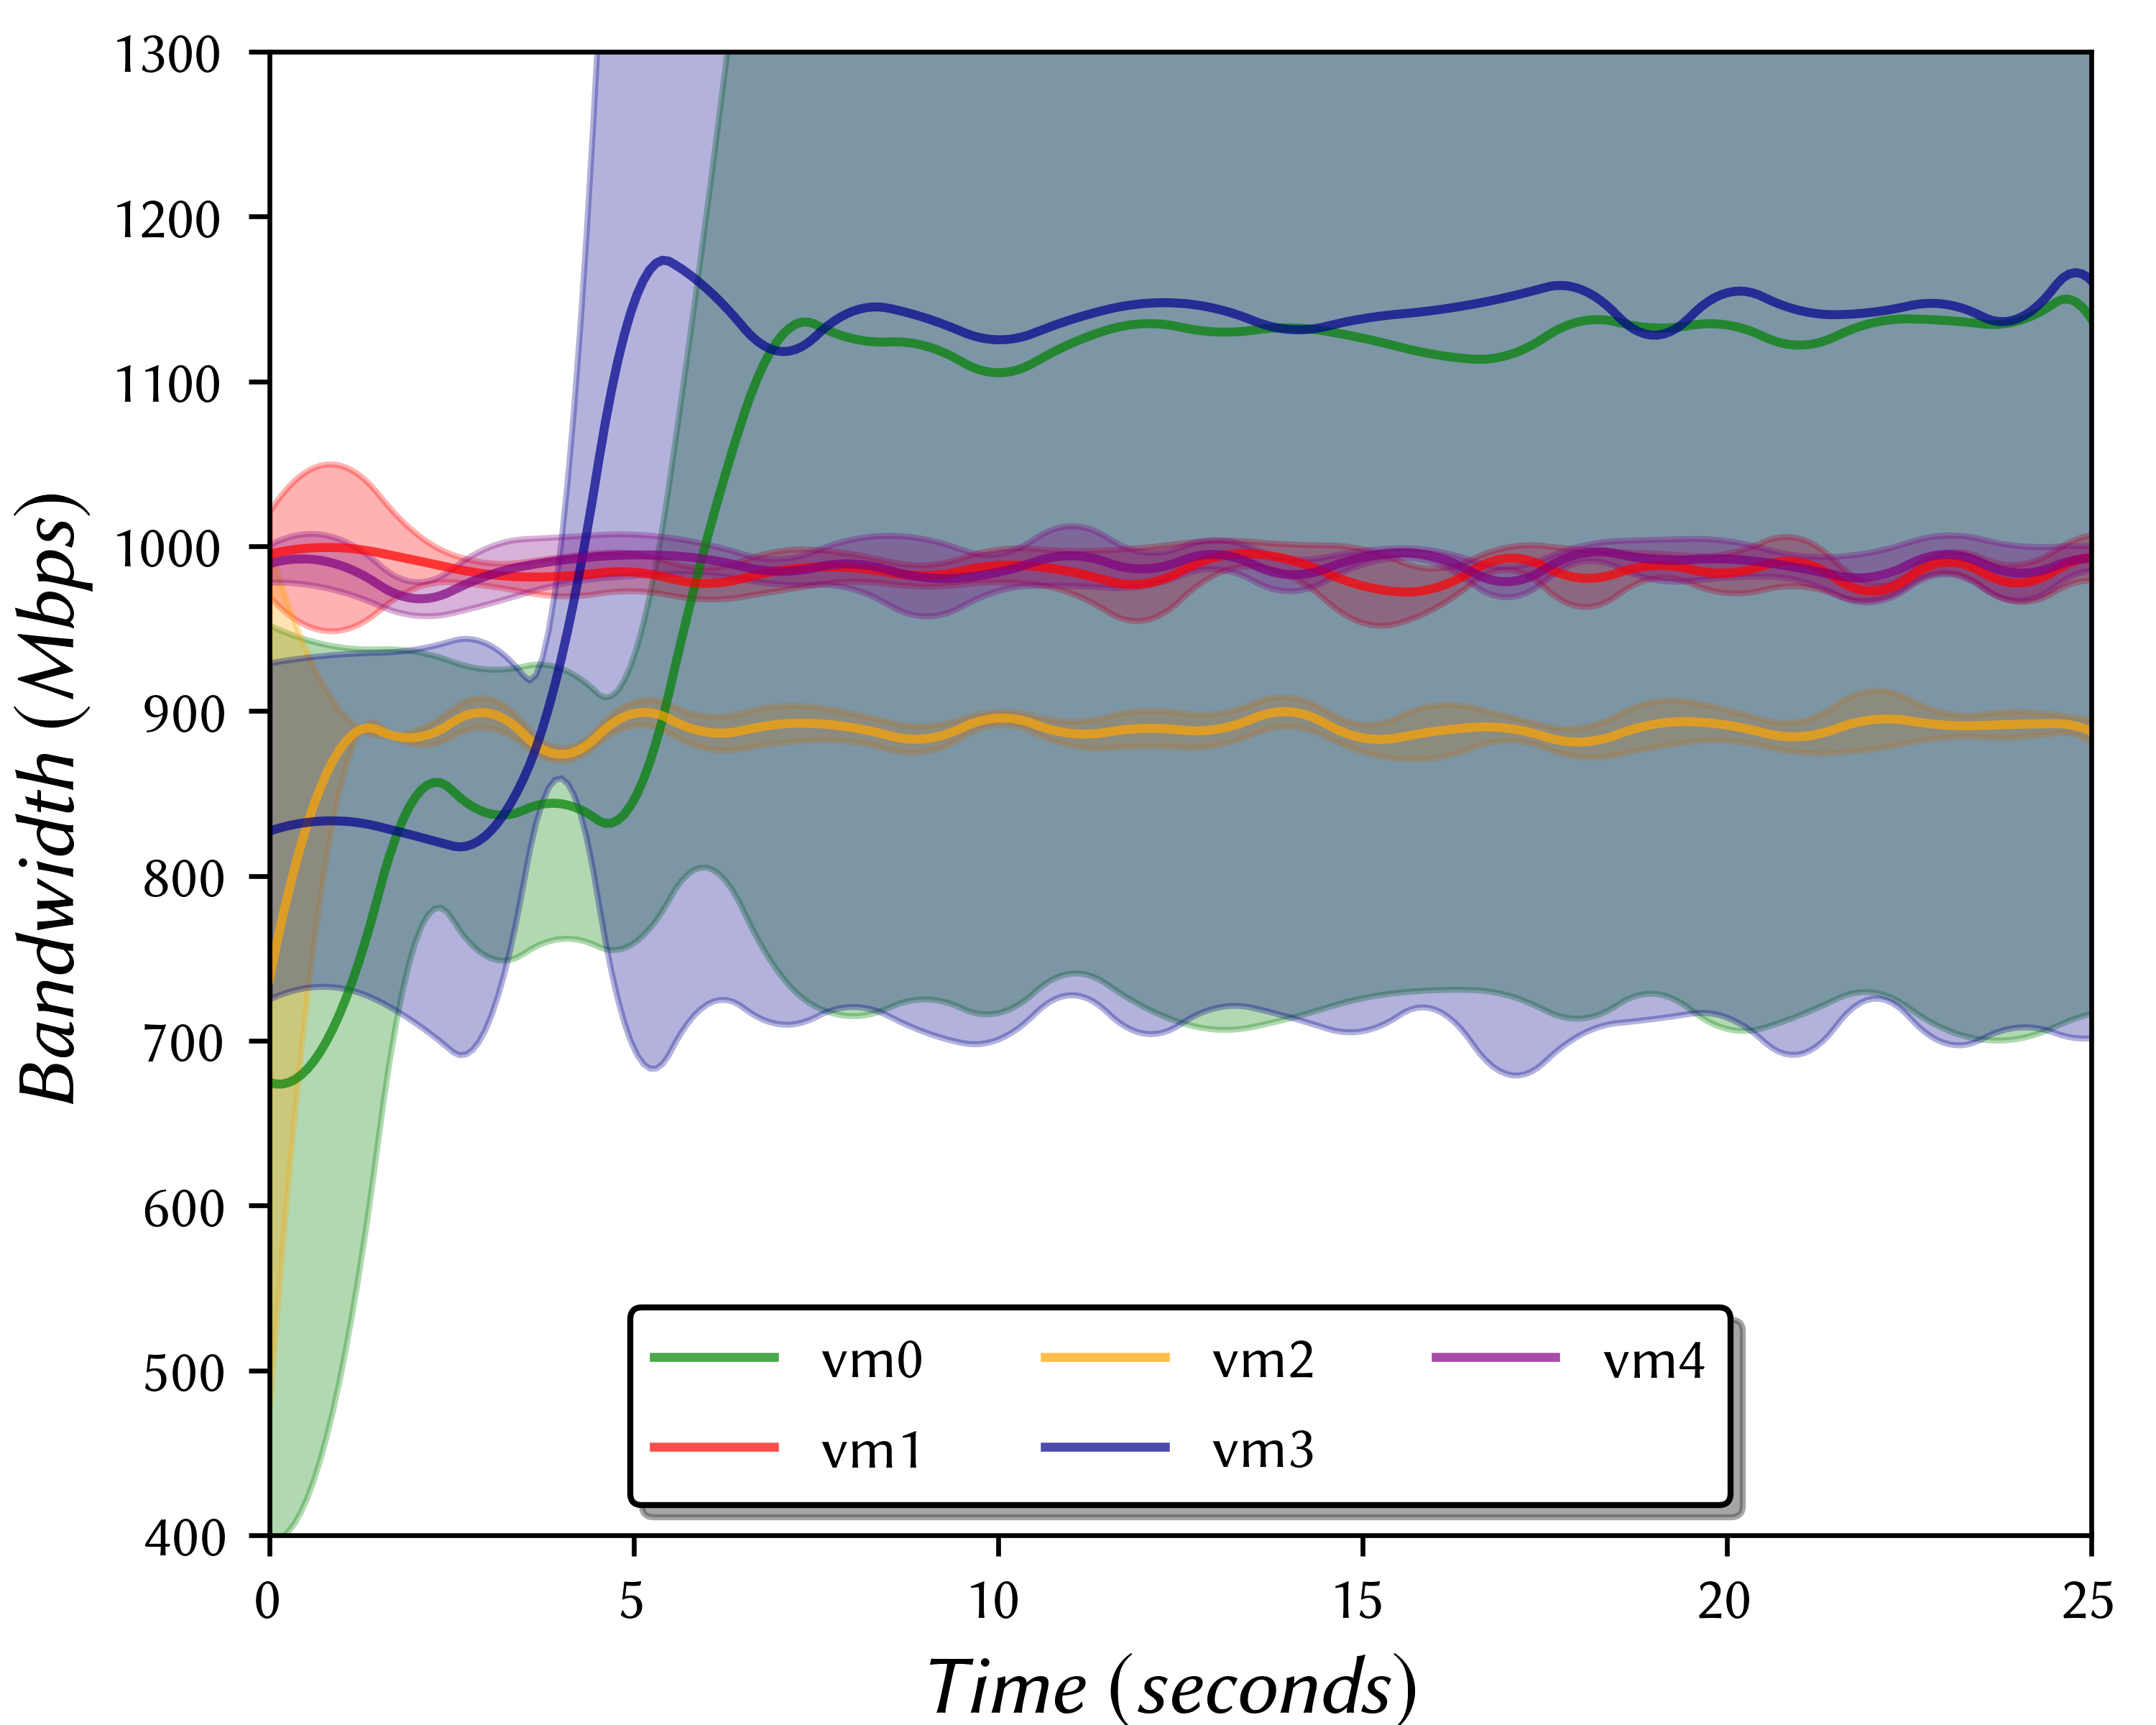
\includegraphics[width=\hsize]{figs/cluster1/setB/vis-3-0.png}
      \vspace{-5mm}
      \caption{Cluster 1}
    \end{subfigure}%
    \hfill
    \begin{subfigure}{.45\textwidth}
      \centering
      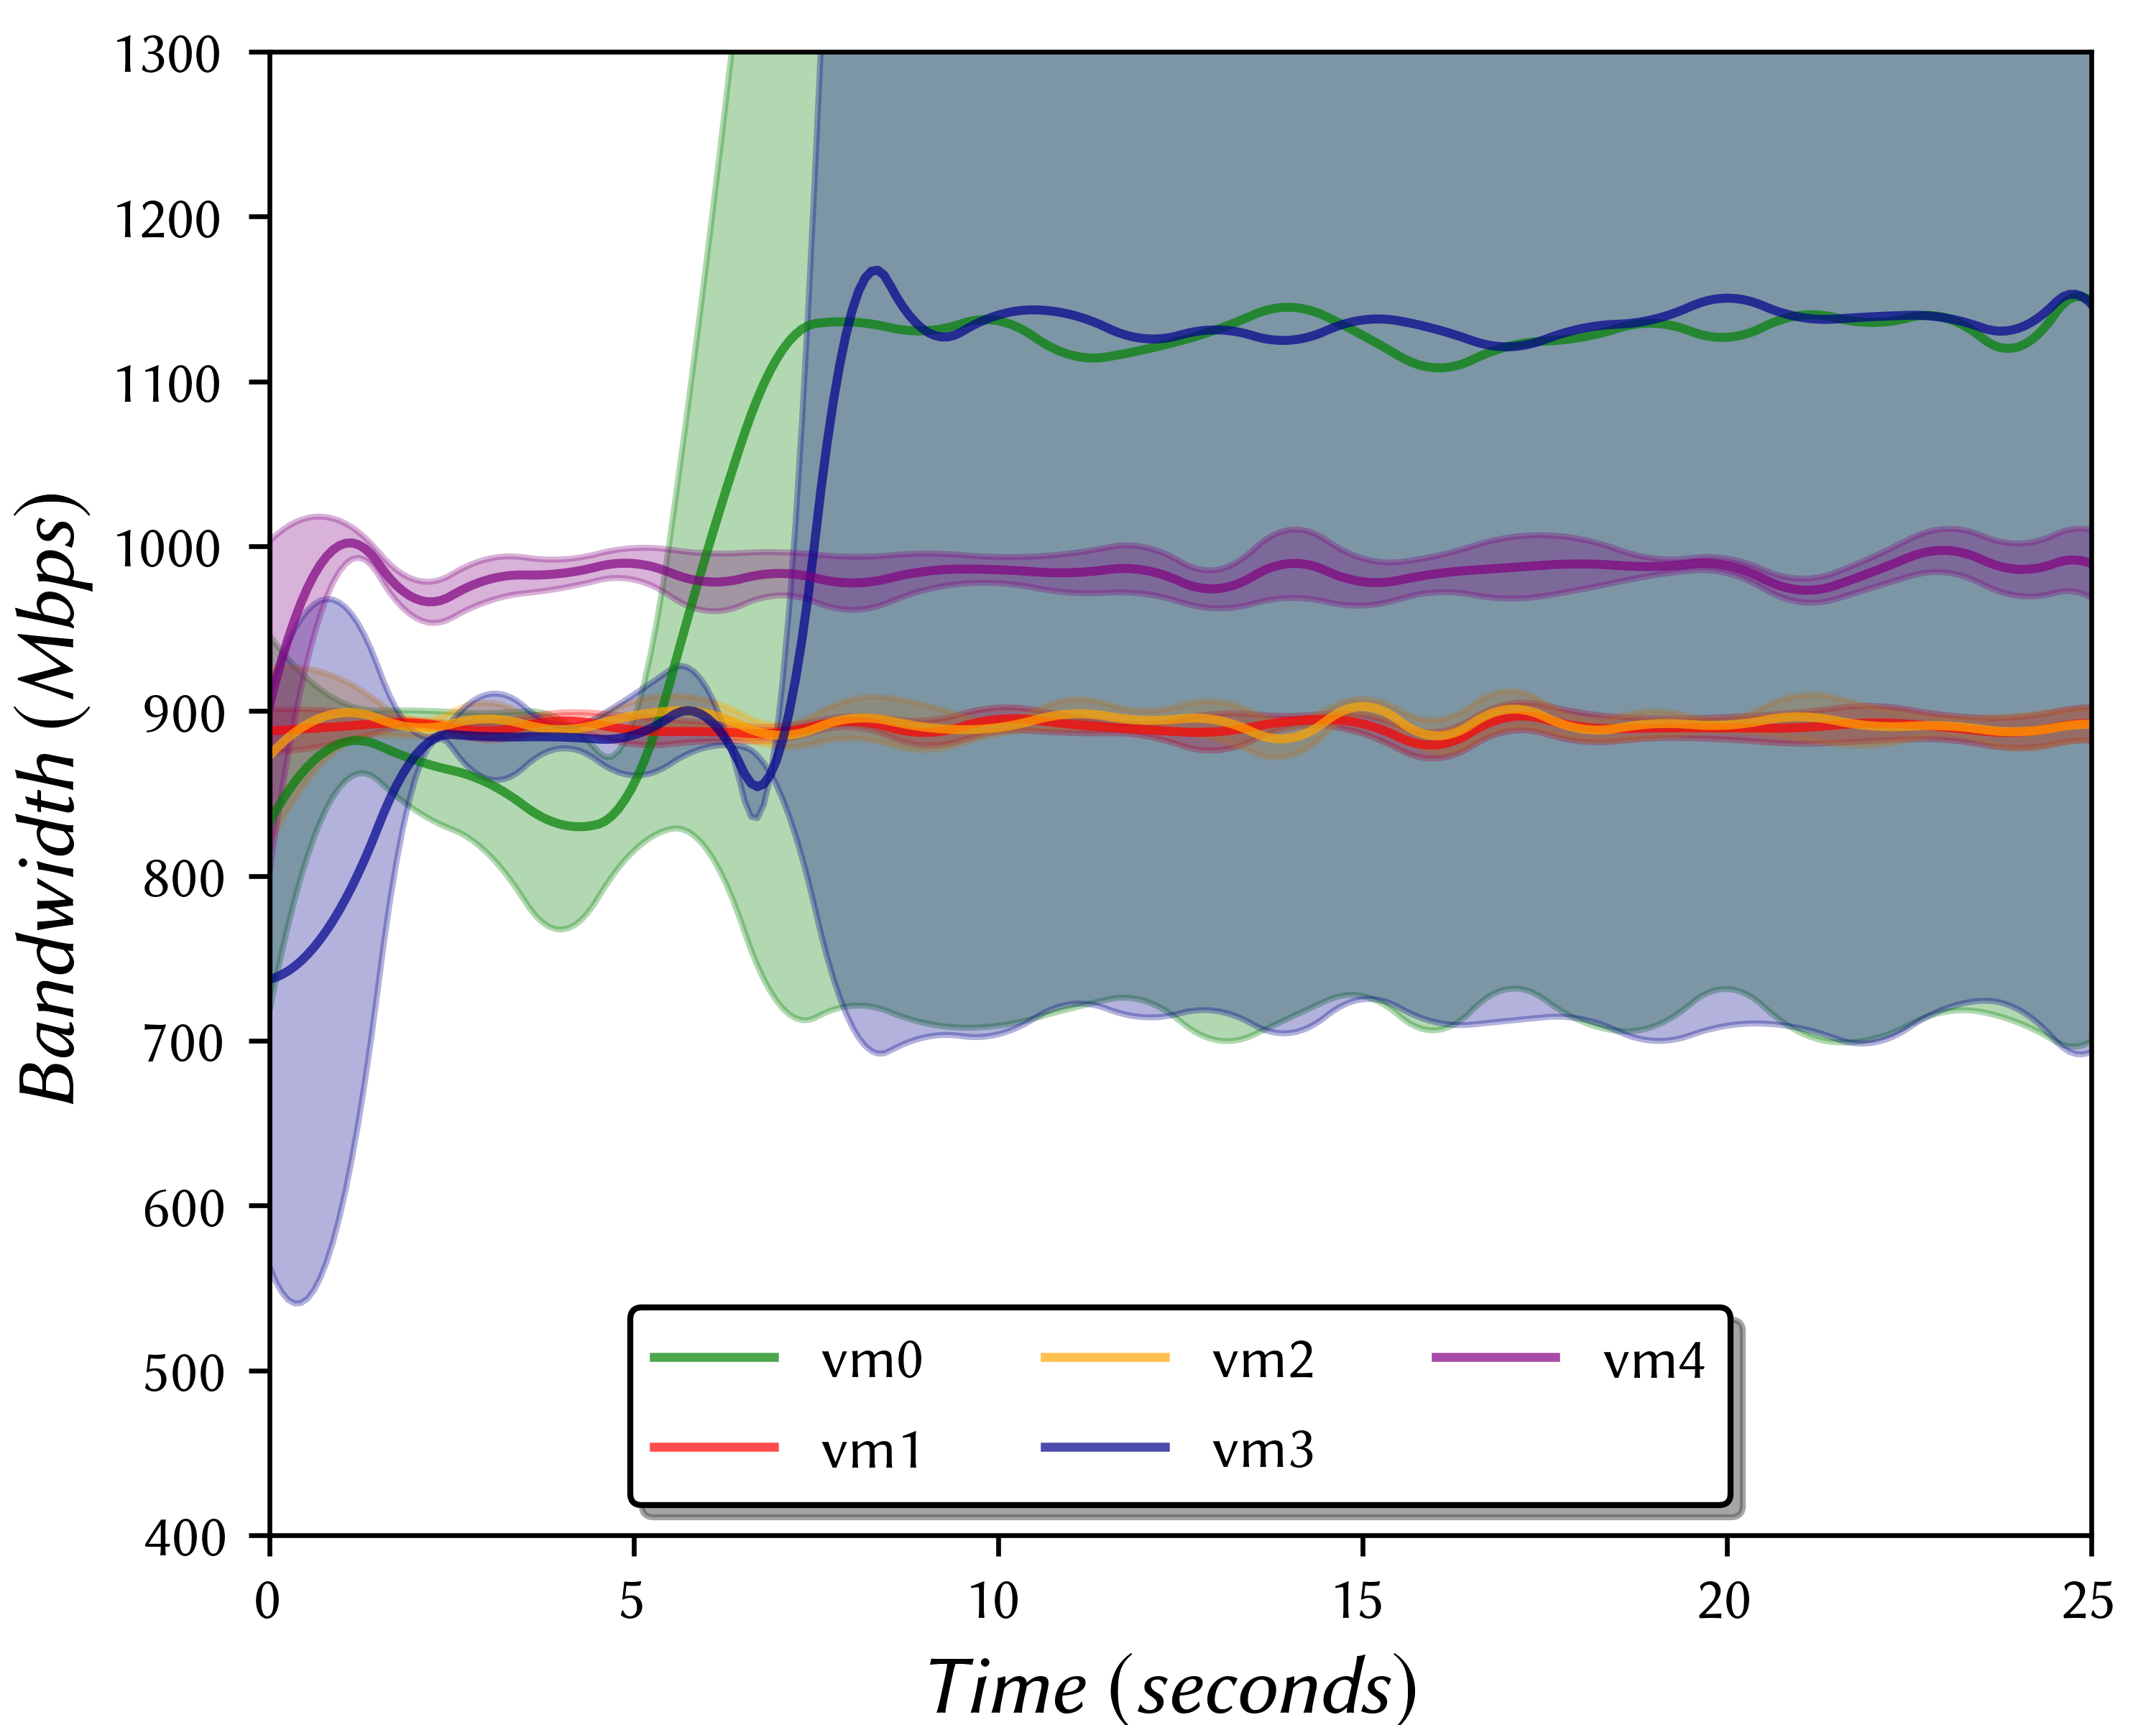
\includegraphics[width=\hsize]{figs/cluster2/setB/vis-3-0.png}
      \vspace{-5mm}
      \caption{Cluster 2}
    \end{subfigure}%
    \caption{\centering{} Experiment 1 TCP bandwidths observed in \texttt{setB}. \\ \texttt{cluster\{1,2\}/setB/d8}, Experiment 1 \\ The first 5 seconds are clipped to allow the network to settle, error bounds are $\pm s$, the sample std. dev.}
    \label{fig:temp-bw-tcp}
\end{figure}

\paragraph{Bandwidth} In \texttt{setA} there was a very clear 1 Gbps maximum egress enforced for each of our VMs, however, as shown in Figure \ref{fig:temp-bw-tcp}, this is no longer the case in \texttt{setB}. In both clusters, $vm0$ and $vm3$ surge up to $\approx$1.15 Gbps with a large amount of variance. On closer inspection of the the \texttt{iperf} output logs, it appears that both VMs can drive $\approx$900 Mbps to $vm1$, $vm2$, and $vm4$, but to each other they peak at $\approx$1.8 Gbps. This relationship is very clearly supported by every run in \texttt{setB} for both clusters.\footnote{Graphs of each run can be found at \texttt{data/cluster\{1,2\}/setB/d\{1..8\}/vis/experiment-1}.}

\paragraph{} To confuse the picture even further, Figure \ref{fig:temp-bw-udp}'s representation of observed UDP bandwidths shows that $vm0$ and $vm3$ fall to the slowest machines, with a rate under half of their peak TCP throughput; \texttt{setA} saw drops between TCP and UDP performance but none as drastic as this. The steps taken by $vm0$ and $vm3$ up to their peaks in Figure \ref{fig:temp-bw-tcp} are interesting --- it appears that the two machines could be negotiating with a third-party, increasing their bandwidths accordingly once approved (this shape is not normal for TCP's rate finding mechanism). Both stepping motions start from a similar position to their UDP performances (circa 700-800 Mbps). Theorising about this relationship, a potential explanation could be that at the bridge between the logical VM and the hypervisor an artificial limit is enforced (as seen from the UDP results). This artificial limit could then be the mechanism the hypervisor uses to allocate more bandwidth to flows of certain traffic classes. Exploring this further is outside the scope of this evaluation, but an approach leveraging tools such as \texttt{tcpreplay} could be used to more accurately synthesise different types of traffic to test this mechanism.


\begin{figure}
    \centering
    \begin{subfigure}{.45\textwidth}
      \centering
      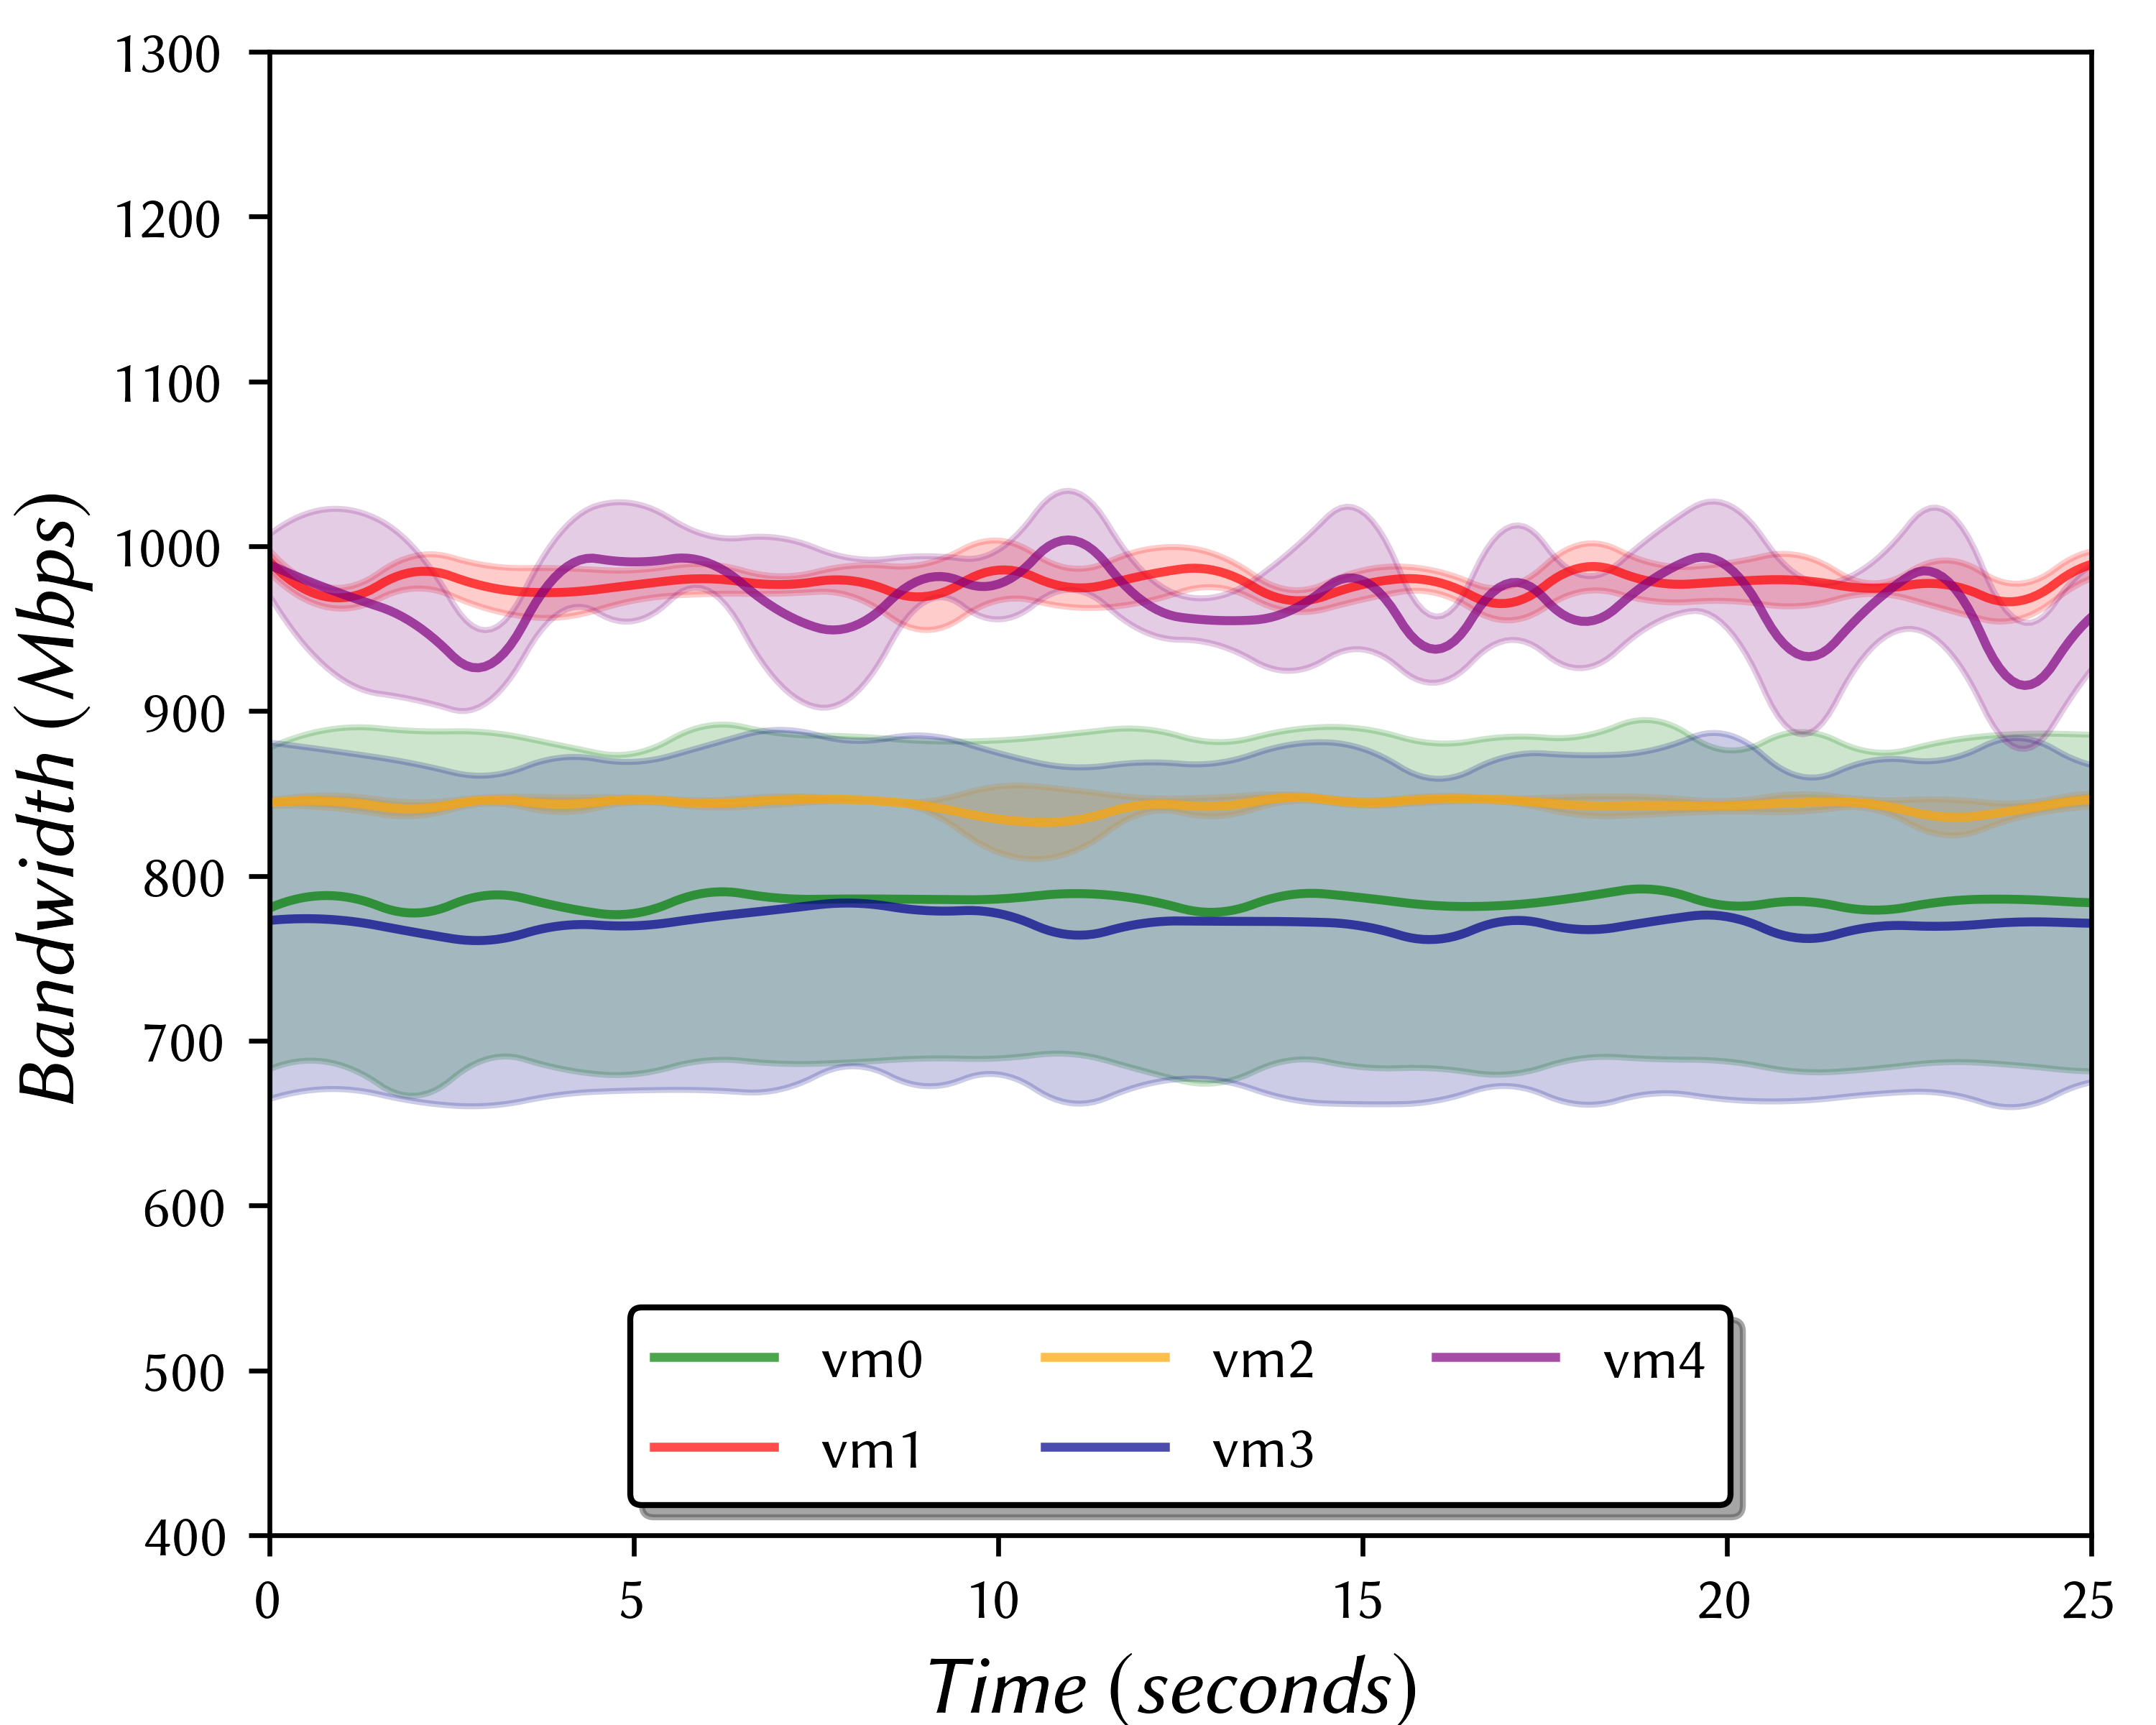
\includegraphics[width=\hsize]{figs/cluster1/setB/vis-3-2.png}
      \vspace{-4mm}
      \caption{Cluster 1}
    \end{subfigure}%
    \hfill
    \begin{subfigure}{.45\textwidth}
      \centering
      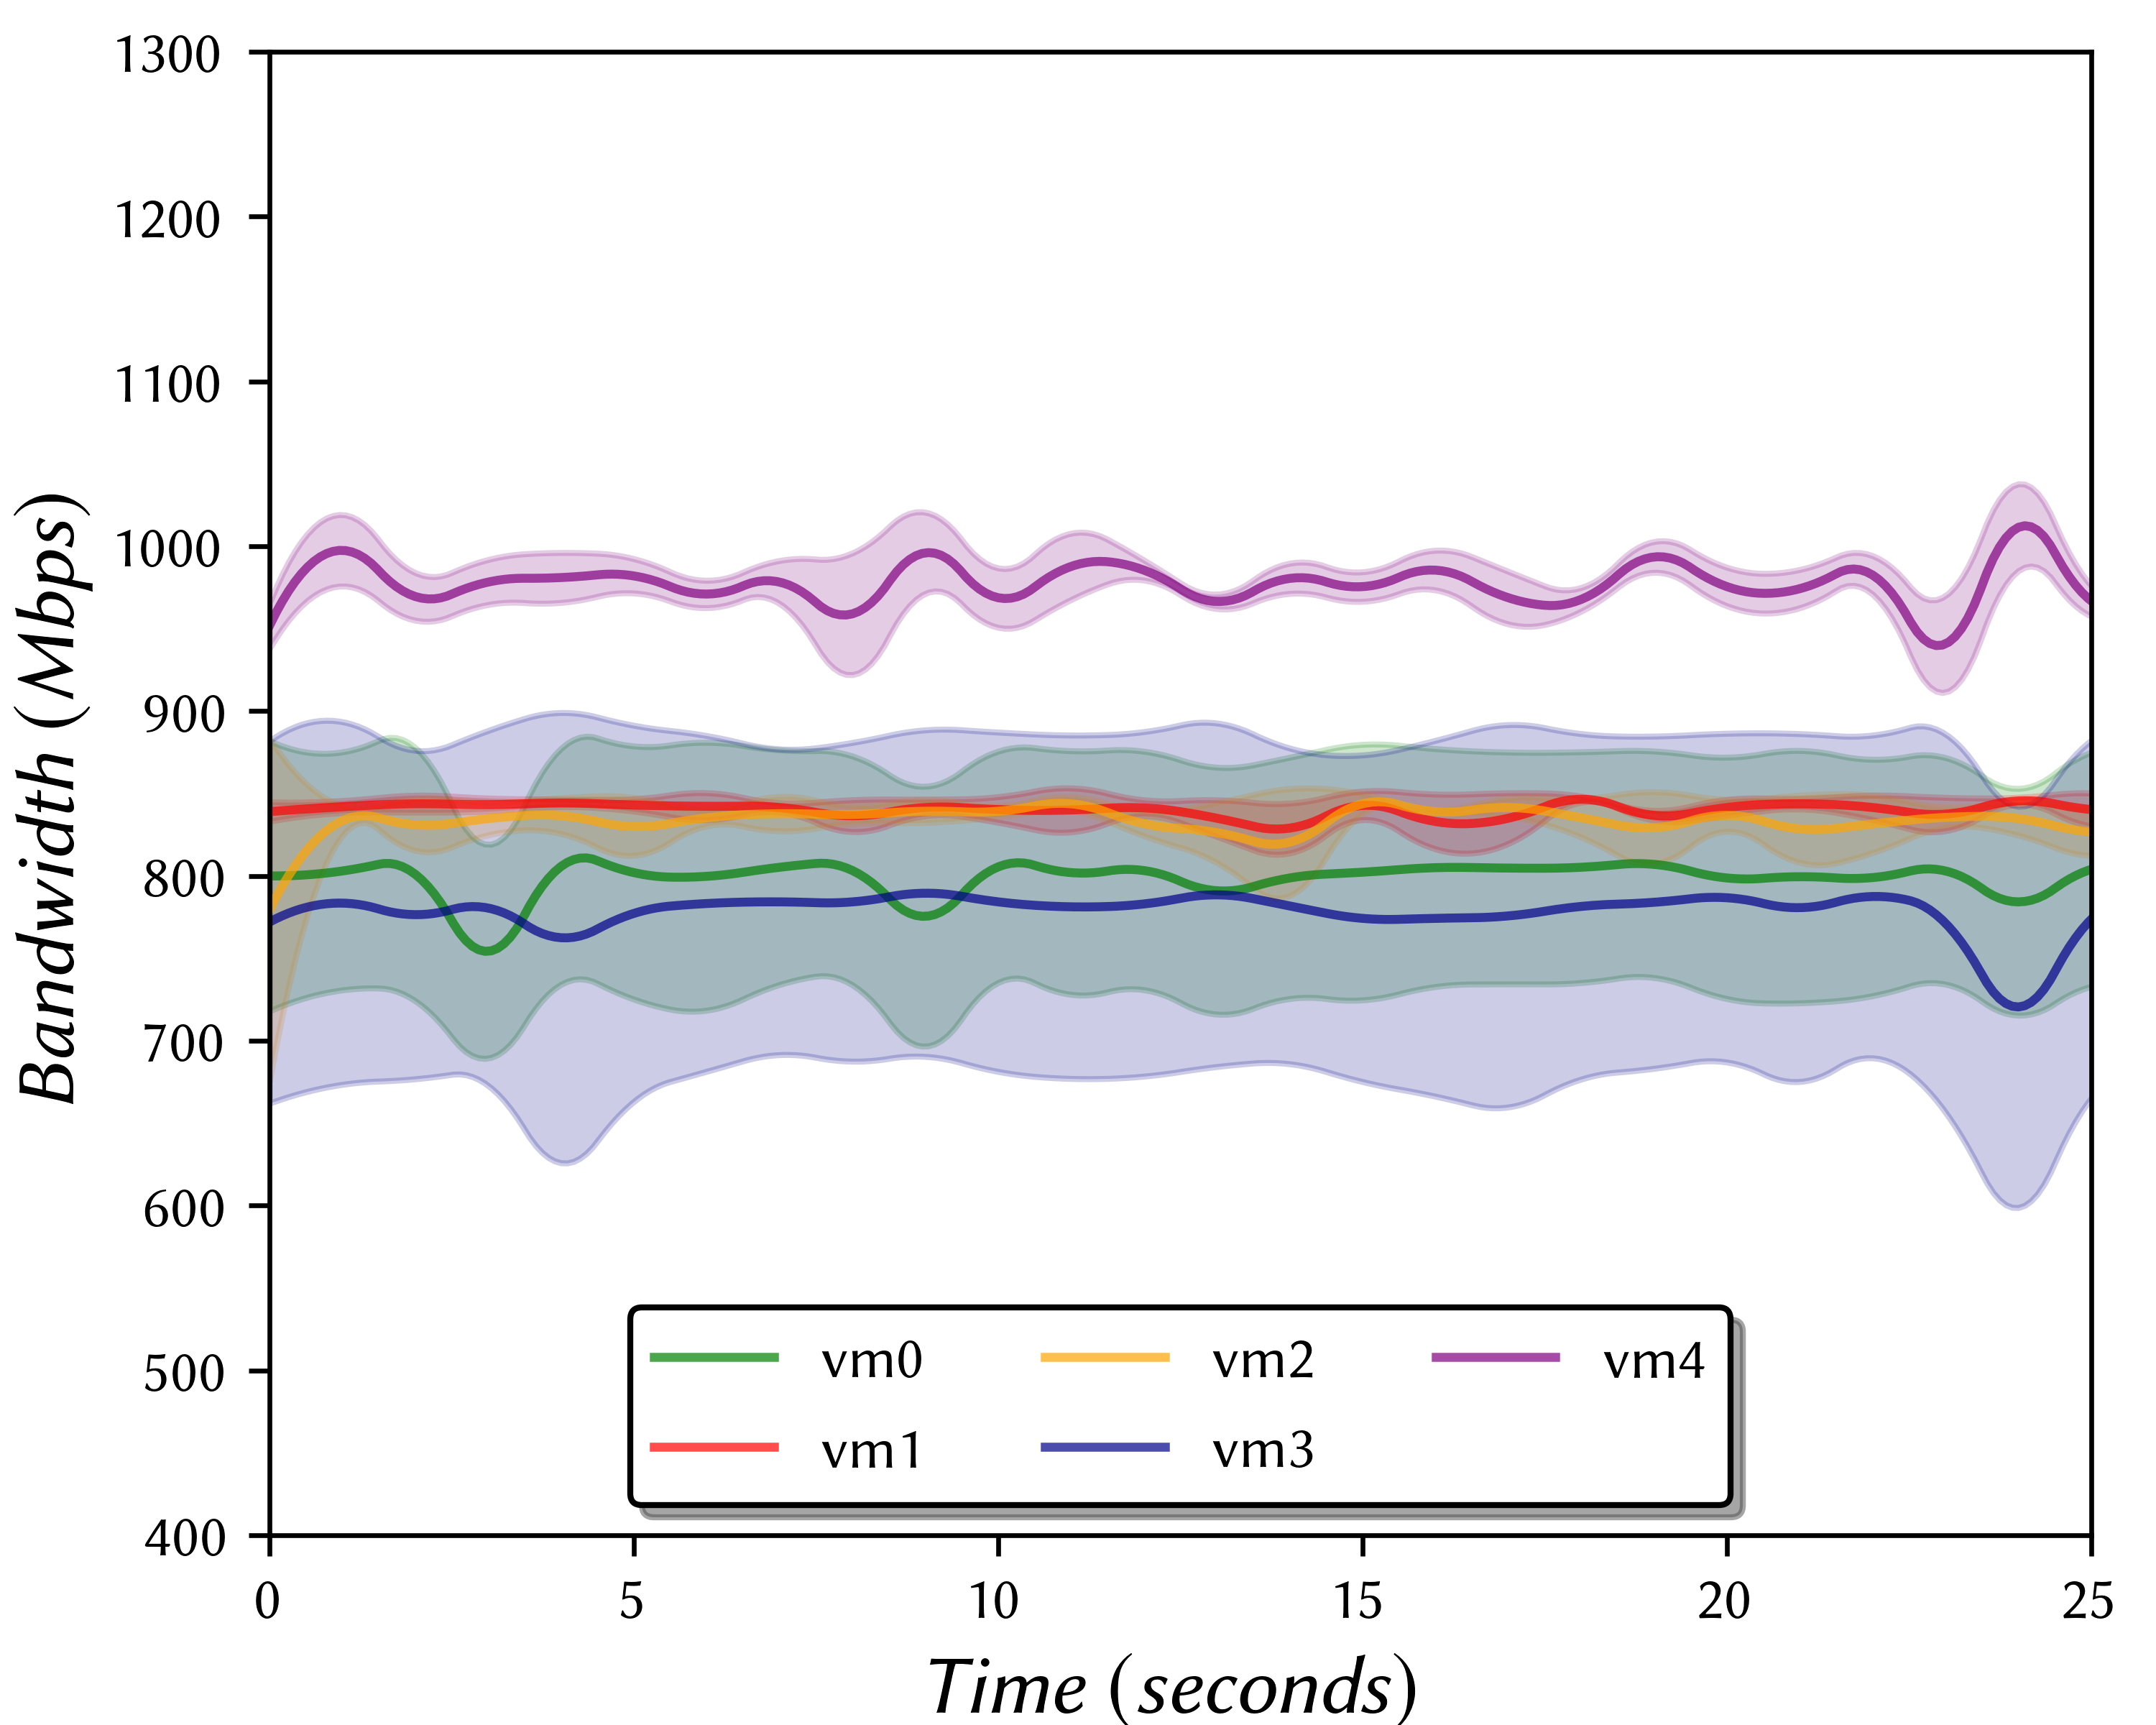
\includegraphics[width=\hsize]{figs/cluster2/setB/vis-3-2.png}
      \vspace{-5mm}
      \caption{Cluster 2}
    \end{subfigure}%
    \caption{\centering{} Experiment 1 UDP bandwidths observed in \texttt{setB}. \\ \texttt{cluster\{1,2\}/setB/d8}, Experiment 1 \\ The first 5 seconds are clipped to allow the network to settle, error bounds are $\pm s$, the sample std. dev.}
    \label{fig:temp-bw-udp}
\end{figure}

\paragraph{} A further question is how does this special relationship between $vm0$ and $vm3$ affect RTTs, particularly with respect to the relative distances between nodes --- Figures \ref{fig:temp-ping-dist-1} and \ref{fig:temp-ping-dist-2} plot this. In Cluster 1 there is a very clear grouping of $vm0$, $vm3$, and, from one direction, $vm4$. This could potentially partially explain this new behaviour, but given Cluster 2 doesn't see the same locality (but does the anomalous behaviour), this seems unlikely.

\paragraph{} Another interesting takeaway from \texttt{setB} is that in Experiment 5, where multiple \texttt{iperf} clients stream to a single machine to test its maximum ingress bandwidth, $vm0$ and $vm3$ both recorded values up to just below 4.5 Gbps, aided by the faster sending rate of the other.

\begin{figure}
\centering
\begin{subfigure}{.21\textwidth}
  \centering
  \includesvg[width=0.9\textwidth,svgpath=./figs/svgs/]{c1-sB-vis-1-small-1e-06-forwards}
  \vspace{5mm}
  \caption{Forward distance plot. (Bottom-left of the matrix)}
  \label{fig:temp-ping-dist-1:a}
\end{subfigure}%
\hfill%
\begin{subfigure}{.21\textwidth}
  \centering
  \includesvg[width=0.85\hsize,svgpath=./figs/svgs/]{c1-sB-vis-1-small-1e-06-backwards}
  \vspace{1mm}
  \caption{Reverse distance plot. (Top-right of the matrix)}
  \label{fig:temp-ping-dist-1:b}
\end{subfigure}%
\hfill%
\begin{subfigure}{.5\textwidth}
  \centering
    \renewcommand{\kbldelim}{(}% Left delimiter
    \renewcommand{\kbrdelim}{)}% Right delimiter
    \[
      \kbordermatrix{
        & vm0 & vm1 & vm2 & vm3 & vm4 \\
        vm0 & - & 0.440 & 0.550 & 0.426 & 0.266 \\
        vm1 & 0.738 & - & 0.505 & 0.629 & 0.628 \\
        vm2 & 0.542 & 0.663 & - & 0.609 & 0.611 \\
        vm3 & 0.311 & 0.535 & 0.588 & - & 0.592 \\
        vm4 & 0.575 & 0.509 & 0.650 & 0.608 & -
      }
    \]
  \vspace{2mm}
  \caption{\centering{} Relative distance matrix between VMs. \\ (Each row is from a single source)}
  \label{fig:temp-ping-dist-1:c}
\end{subfigure}
\caption{\centering{} Cluster 1 \texttt{ping} $\,$RTT relative distances approximation.  \\ \texttt{cluster1/setB/aggr}, $\,$Experiment 2, Interval = $10^{-6}$s}
\label{fig:temp-ping-dist-1}
\end{figure}

\begin{figure}
\centering
\begin{subfigure}{.21\textwidth}
  \centering
  \includesvg[width=0.8\textwidth,svgpath=./figs/svgs/]{c2-sB-vis-1-small-1e-06-forwards}
  \vspace{3mm}
  \caption{Forward distance plot. (Bottom-left of the matrix)}
  \label{fig:temp-ping-dist-2:a}
\end{subfigure}%
\hfill%
\begin{subfigure}{.21\textwidth}
  \centering
  \includesvg[width=\hsize,svgpath=./figs/svgs/]{c2-sB-vis-1-small-1e-06-backwards}
  \vspace{2mm}
  \caption{Reverse distance plot. (Top-right of the matrix)}
  \label{fig:temp-ping-dist-2:b}
\end{subfigure}%
\hfill%
\begin{subfigure}{.5\textwidth}
  \centering
    \renewcommand{\kbldelim}{(}% Left delimiter
    \renewcommand{\kbrdelim}{)}% Right delimiter
    \[
      \kbordermatrix{
        & vm0 & vm1 & vm2 & vm3 & vm4 \\
        vm0 & - & 0.609 & 0.635 & 0.580 & 0.431 \\
        vm1 & 0.619 & - & 0.652 & 0.493 & 0.581 \\
        vm2 & 0.546 & 0.464 & - & 0.528 & 0.513 \\
        vm3 & 0.573 & 0.637 & 0.324 & - & 0.549 \\
        vm4 & 0.642 & 0.592 & 0.555 & 0.578 & -
      }
    \]
  \vspace{1mm}
  \caption{\centering{} Relative distance matrix between VMs. \\ (Each row is from a single source)}
  \label{fig:temp-ping-dist-2:c}
\end{subfigure}
\caption{\centering{} Cluster 2 \texttt{setB} \texttt{ping} $\,$RTT relative distances approximation.  \\ \texttt{cluster2/setB/aggr}, $\,$Experiment 2, Interval = $10^{-6}$s}
\label{fig:temp-ping-dist-2}
\end{figure}

\newpage
\section{Reproducing Results}
\label{sec:reproducability}

\paragraph{} This section provides an in-depth look at how the evaluation framework functions, with a particular focus on documenting how to use it to run and recreate the experiments shown in this report.

\paragraph{Preparing the Environment} To prepare the cluster to run the framework you need to first choose a master node; I chose $vm0$ for both clusters. Obtaining the framework can done by simply running the following command on the master;

\vspace{-4mm}
\begin{align*}
    \texttt{bash <(curl -s https://comps.ci/f4cGJM+)}
\end{align*}

\paragraph{} This clones the \texttt{git} repository and runs the \texttt{init.sh} script.\footnote{To verify what this does go to the URL to view the script's source.} The \texttt{init.sh} script ensures that all of the framework's required dependencies are installed, and sets up environment as required; the framework will be placed in the \texttt{$\sim$/x} directory. Next we need to prepare the other VMs in the cluster: this is achieved using the \texttt{init-remote.sh} script, which ensures the framework is present on the machine, that both machines share an SSH key, and runs \texttt{init.sh}. For example, to initialise all other machines in Cluster 1, the following command was used.

\vspace{-4mm}
\begin{align*}
    \texttt{for i in \{5..8\}; do $\sim$/x/init-remote.sh 10.0.0.\$i; done}
\end{align*}

\paragraph{} Once all of the other VMs have been successfully set up we can start to run experiments.

\paragraph{Running an Experiment} The \texttt{$\sim$/x/experiments/} folder contains all of the Python files required to run experiments; \texttt{definitions.yml} file holds all of the experiment definition and parameter sets. Running experiment 1 against 10.0.0.5 and 10.0.0.6, for example, is done with;

\vspace{-4mm}
\begin{align*}
    \texttt{python3 experiment.py -e 1 -t 10.0.0.5,10.0.0.6}
\end{align*}

\paragraph{} Running all experiments is done using;

\vspace{-4mm}
\begin{align*}
    \texttt{python3 experiment.py -e 0 -t 10.0.0.5,10.0.0.6,10.0.0.7,10.0.0.8}
\end{align*}

\paragraph{} Once execution has completed, the results are put into \texttt{$\sim$/x/experiments/results} --- the \texttt{contents} file is a log of all experiments run and the unique ID assigned to them (this is also printed at the end of running \texttt{experiment.py}). This ID then acts as the folder index in \texttt{$\sim$/x/experiments/results/data/}.

\paragraph{} The general structure of a results folder is as follows. \texttt{\$id} is the unique ID mentioned above, \texttt{\$i} the experiment number, \texttt{\$parameter\_set} the index of the parameter set used in \texttt{definitions.yml}, and \texttt{\$target\_ip} the IP of the target VM.

\vspace{-4mm}
\begin{align*}
    \texttt{/ \$id-experiment-\$i / \$parameter\_set / \$target\_ip}
\end{align*}

\paragraph{} In every folder there is either an \texttt{overview} or \texttt{explain} file; this, as you may have guessed, given a brief explanation of what the framework was doing when it produced the data in that folder.

\paragraph{} The leaves at the bottom of every experiment folder are the \texttt{local} or \texttt{remote} files. These are the local and remote outputs produced when running the experiment. When there are multiple these are suffixed with either an index or the relevant VM's IP address.

\paragraph{Automate Distributing Experiments} In order to get regular snapshots of the clusters' performance, all experiments need to be run regularly from every single VM in turn. This function is provided by the distribution module in \texttt{$\sim$/x/distribute/}. The syntax is exactly the same as \texttt{experiment.py}, but will create a sequential chain of invocation across all specified machines and repatriate the produced data.

\vspace{-4mm}
\begin{align*}
    \texttt{python3 distribute.py -e 0 -t 10.0.0.5,10.0.0.6,10.0.0.7,10.0.0.8}
\end{align*}

\paragraph{} Once execution has completed both locally and remotely on all other VMs, the results from all hosts will be available in \texttt{$\sim$/x/distribute/results/}. Each folder is named \texttt{dX}, where \texttt{X} is a simple increasing index. Inside each \texttt{dX} is one folder per VM specified as a target.

\paragraph{} For reference, a distributed experiment takes roughly 2.5 hours to complete with 5 hosts. The evaluations that generated the accompanying data sets from the clusters were automated using a \texttt{cron} job to send a command to a waiting \texttt{tmux} session; this allowed execution to continue as normal even in the absence of a login shell.

\paragraph{Analysing the Results} The final module, in \texttt{$\sim$/x/analysis/}, simply takes the output from the distribution module (\texttt{dX} folders) and renders the various graphs designed for this report. To test, take the experiment data dump provided alongside this submission (it should produce a single folder, \texttt{data/}), and put it in the \texttt{$\sim$/x/analysis/} folder. Note that the generated graphs are already included and will be overwritten by running the following commands. Graphs are generated using;

\vspace{-4mm}
\begin{align*}
    \texttt{python3 analyse.py -c 1 -p data/cluster1/setA/d8}
\end{align*}

\paragraph{} To generate all individual graphs the following script can be used;

\vspace{-4mm}
\begin{align*}
    & \texttt{for c in \{1..2\}; do} \\
    & \quad \texttt{for s in \{A,B\}; do} \\
    & \quad \quad \texttt{for i in \{1..8\}; do}\\
    & \quad \quad \quad \texttt{python3 analyse.py -c \$c -p data/cluster\$c/set\$s/d\$i;} \\
    & \quad \quad \texttt{done;} \\
    & \quad \texttt{done;} \\
    & \texttt{done;}
\end{align*}

\paragraph{} The analysis tools also provide the ability to aggregate results over a number of experiment runs; this is activated by simply specifying a list of paths to the \texttt{-p} flag. For example;

\vspace{-4mm}
\begin{align*}
    \texttt{python3 analyse.py -c 1 -p data/cluster1/setA/d7 data/cluster1/setA/d8}
\end{align*}

\paragraph{} Or, more concisely;

\vspace{-4mm}
\begin{align*}
    \texttt{for i in \{1..2\}; do python3 analyse.py -c \$i -p data/cluster\$i/setA/d\{1..8\}; done}
\end{align*}

\paragraph{} Table \ref{table:vis} describes every visualisation produced by \texttt{analyse.py}. 150 graphs are generated for every distributed experiment execution --- this takes the total number of graphs for all of the attached recorded data to just under 5,000. It is probably not advisable to re-render all the graphs, as this can take quite some time.  

\begin{table}
\centering
\bgroup
    \def\arraystretch{1.5}%
    \begin{tabularx}{\textwidth}{r|X}
    \textbf{Visualisation} & Description \\
    \hline
    \textbf{experiment-2/vis-1} & The RTT relative distance plots for all parameter set combination. As seen, for example, in Figure \ref{fig:ping-dist-1:a}. \\ 
    \textbf{experiment-2/vis-2} & The all-to-all \texttt{ping} RTT matrix; for example, Figure \ref{fig:ping-c1}. \\ 
    \textbf{experiment-1/vis-3} & The averaged bandwidths seen across all VMs, indexed by parameter set index; for example, Figure \ref{fig:bw-1}. \\ 
    \textbf{experiment-1/vis-4} & TCP vs UDP bandwidth for all VMs (large vs small packet sizes). \\ 
    \textbf{experiment-4/vis-5} & Bidirectional \texttt{iperf} plots; for example, Figure \ref{fig:bw-bidir-1}. \\ 
    \textbf{experiment-5/vis-6} & Simple plot of the results from the multi-ingress \texttt{iperf} tests; vis-8 is the aggregated form of this. \\ 
    \textbf{experiment-6/vis-7} & Simple plot of the results from the multi-egress \texttt{iperf} tests; vis-9 is the aggregated form of this. \\ 
    \textbf{experiment-5/vis-8} & Aggregated multi-ingress \texttt{iperf} tests, indexed by the number of incoming streams. For example, Figure \ref{fig:bw-n-1-1}. \\ 
    \textbf{experiment-6/vis-9} & Aggregated multi-egress \texttt{iperf} tests, indexed by the number of outgoing streams. For example, Figure \ref{fig:bw-1-n-1}. \\ 
    \end{tabularx}
    \egroup
    \caption{Description of the visualisations produced by \texttt{analyse.py}.}
    \label{table:vis}
\end{table}

% \bibliography{refs}{}
% \bibliographystyle{unsrt}
% \clearpage
% \appendix
% \section{Reproducability Report}

\end{document}